\title{Variational and Diffusion Monte Carlo approaches to the nuclear few- and many-body problem}
\author{Francesco Pederiva, Alessandro Roggero, Kevin E. Schmidt}
\institute{Francesco Pederiva \at Physics Department, University of Trento, and INFN-TIFPA, Trento, Italy , \email{francesco.pederiva@unitn.it} \and Kevin E. Schmidt \at Department of Physics, Arizona State University, Tempe AZ 85283-1506 (USA) \email{kevin.schmidt@asu.edu} \and
Alessandro Roggero \at Institute for Nuclear Theory, University of Washington, Seattle WA (USA) , \email{roggero@uw.edu}}

\maketitle
\abstract{We review Quantum Monte Carlo methods, a class of stochastic methods allowing for solving the many-body Schr\"odinger equation for an arbitrary Hamiltonian. The basic elements of
the stochastic integration theory are first presented, followed by the implementation to the
variational solution of the quantum many-body problem. Projection algorithms are then introduced, beginning with a formulation in coordinate space for central potentials, in order to illustrate
the fundamental ideas. The extension to Hamiltonians with an explicit dependence on the spin-isospin degrees of freedom is then presented by making use of auxiliary fields (Auxiliary Field Diffusion Monte Carlo, AFDMC). Finally, we present the Configuration Interaction Monte Carlo algorithm (CIMC) a method to compute the ground state of general, local or non-local, Hamiltonians based on the configuration space sampling.}

\label{chapter:qmc}
%\maketile


\section{Monte Carlo methods in quantum many-body physics}
\subsection{Expectations in Quantum Mechanics}
In the previous chapters the authors pointed out in several different ways that the non-relativistic quantum many-body problem 
is equivalent to the solution of a very complicated differential equation, the many-body Schr\"odinger equation.

As it was illustrated, in the few-body case ($A<6$) it possible to find compute exact solutions. At the very least, one can expand the eigenfunctions on a basis set including $\cal M$ elements,
diagonalize the Hamiltonian matrix, and try to reach convergence as a function of $\cal M$. Unfortunately, this procedure becomes more and more expensive
when the number of bodies $A$ increases. There are many ingenuous ways to improve the speed of convergence and the quality of the results. The price to pay often is the introduction of more or less controlled approximations.

All these approaches have one common feature: they end up with some closed expression for the eigenfunctions. However, we should remember that the wavefunction {\it per se} is not an observable. In order to make predictions to be compared with experiments, we only need a way to compute {\it expectations} of operators $\hat{O}$ describing the observables we are interested in. 

Given a many-body Hamiltonian $\hat{H}$, we might want, for instance, to look for the ground state eigenfunction and eigenvalue. This means that we want to solve the following equation:
\begin{equation}
\label{eqchap9.s}
\hat{H}\vert \Psi_0\rangle=E_0\vert \Psi_0\rangle.
\end{equation}  
At this point we to provide a representation of the Hilbert space in term of some basis set.
This set will be denoted as $\{|X\rangle\}$. Its elements could be eigenstates of the position
or of the momentum operators, or eigenstates of a simpler Hamiltonian of which we know the exact spectrum. 
In order to make the notation less cumbersome, we will assume that the quantum numbers $X$ characterizing the basis states are in the continuum. In the case of a discrete spectrum, integrals in the following have to be replaced by sums over all their possible values, without any loss of generality. As an example, $X$ could include the positions or the momenta of $A$ nucleons, and their spin and isospin values.  

All the physical information we need about the time-independent problem is then included in integrals of the form:
\begin{equation}
\langle O\rangle \equiv\langle \Psi_0\vert\hat{O}\Psi_0\rangle =\frac{\displaystyle\int\; dX dX'\langle \Psi_0\vert X\rangle\langle X\vert \hat{O}\vert X'\rangle\langle X'\vert\Psi_0\rangle}
{\displaystyle\int\; dX \vert\langle X\vert \Psi_0\rangle\vert^2}.
\end{equation}


These integrals are apparently as hard to solve as the Schr\"odinger equation itself, even if we had access to the explicit form of the wavefunction. Is there any real gain in reformulating the problem this way?

We can first notice that expectations can in general be written in a slightly different form, independent of the nature of the operator $\hat{O}$:
\begin{equation}
\langle O\rangle =\displaystyle\frac{\displaystyle\int\; dX \vert \langle X\vert \Psi_0\rangle\vert^2\displaystyle\displaystyle\frac{\langle X \vert \hat{O}\Psi_0\rangle}{\langle X\vert \Psi_0\rangle}}{\displaystyle\int\; dX \vert\langle X \vert \Psi_0\rangle \vert^2}.
\end{equation}
For the moment we will just assume that the quotient appearing at numerator of the expectation is always well defined, and we will later discuss this aspect in more detail.
The standard quantum mechanical interpretation of the wavefunction tells us that the quantity:
\begin{equation}
P[X]=\frac{\vert \langle X\vert \Psi_0\rangle\vert^2}{\displaystyle\int\; dX \vert\langle X \vert \Psi_0\rangle \vert^2},
\end{equation}  
is the probability density of finding the system in the state $\vert X \rangle$ labeled by the set of quantum numbers $X$. Thereby, the expectation integral has the general form:
\begin{equation}
\langle O\rangle =\int\; dX P[X]\displaystyle\frac{\langle X \vert \hat{O}\Psi_0\rangle}{\langle X\vert \Psi_0\rangle},
\label{eq5}
\end{equation}
i.e. the average of what we will call the {\it local} operator $O_{loc}\equiv \frac{\langle X \vert \hat{O}\Psi_0\rangle}{\langle X\vert \Psi_0\rangle}$ weighted with the probability of finding the system in a given state $\vert X\rangle$. 
Integrals like that in Eq. (\ref{eq5}) have a direct physical interpretation. In a measurement process what we would observe is essentially the result of a {\it sampling process} of $P[X]$. The expectation of our operator is approximated by:
\begin{equation}
\langle O \rangle \simeq \frac{1}{M}\sum_{k=1}^M{O(X_k)},
\end{equation}
where $M$ is the number of measurements performed, and $O(X_k)$ is a shorthand notation to 
indicate the value assumed by the observable $\hat{O}$ in the state labeled by the quantum numbers $X_k$. The laws of statistics also give us a way of estimating a {\it statistical} error on $\langle O \rangle$, and we know that the error decreases by increasing 
the number of measurements. 

There is here an important point to notice: in a physical measurement process we have {\it no direct knowledge  of the wavefunction}, we just {\it sample} its squared modulus! 

This argument suggests that if we had a numerical way of sampling the squared modulus of a wavefunction, we could in principle compute expectations and make comparisons with experiments
without needing an explicit expression of the wavefunction itself. Quantum Monte Carlo methods
aim exactly at solving the many-body Schr\"odinger equation by sampling its solutions, eventually
without any need of an explicit analytical form.

The remainder of this chapter will be organized as follows. First we will discuss
how to perform calculations based on an accurate, explicit ansatz for the wavefunction of an $A$-body system interacting via a purely central potential, exploiting the variational principle of quantum mechanics (Variational Monte Carlo methods). Then we will discuss how to sample the exact ground state of the system by
projecting it out of an initial ansatz (Projection Monte Carlo methods). Finally, we will
see how these methods need to be extended when we are interested in studying Hamiltonians
that have an explicit dependence on the spin and isospin states of the particles, as it 
happens for the modern interactions employed in nuclear physics.

\section{Variational wavefunctions and VMC for central potentials}



\subsection{Coordinate space formulation}
As previously discussed, we are in principle free to choose any representation of the Hilbert
space of the system we like, in order to compute expectations. The most convenient choice, for a system of particles interacting via a purely central potential, with no explicit dependence on the spin or isospin state, is to use the eigenstates of the
position operator. If $R={{\bf r}_1,\dots{\bf r}_A}$ are the coordinates of the $A$ 
(identical)\footnote{We will always refer to systems of identical particle throughout the text. The generalization to mixtures is normally straightforward, and it will not be discussed here.} particles of mass $m$ constituting the system, we have that:
\begin{equation}
\vert X\rangle \equiv \vert R \rangle
\end{equation}
with the normalization:
\begin{equation}
\langle R'\vert R\rangle = \delta(R-R') \,.
\end{equation}
Notice that we are here considering a $3A$-dimensional Cartesian space, without decomposing it
in the product of $A$ $3$-dimensional spaces. In this representation the wavefunction 
is simply given by:
\begin{equation}
\langle R\vert\Psi_0\rangle \equiv \Psi_0(R)=\Psi_0({\bf r}_1,\dots{\bf r}_A).
\end{equation}
The Hamiltonian instead reads:
\begin{equation}
\hat{H}=\sum_{i=1}^A \frac{p_i^2}{2m}
+V({\bf r}_1,\dots{\bf r}_A),
\end{equation}
or
\begin{equation}
\hat{H} = \int dR \vert R\rangle
\left [
-\frac{\hbar^2}{2m}\sum_{i=1}^A \nabla^2_i +V({\bf r}_1,\dots{\bf r}_A)
\right ] \langle R\vert\,,
\end{equation}
where $V$ is the interparticle potential. 
Substituting this form into Eq. (\ref{eqchap9.s}), operating from the
left with $\langle R\vert$ gives the Schr\"odinger differential equation
\begin{equation}
\left [
-\frac{\hbar^2}{2m}\sum_{i=1}^A \nabla^2_i +V({\bf r}_1,\dots{\bf r}_A)
\right ] \Psi_0(R) = E_0\Psi_0(R) \,.
\end{equation}
We will often use the same symbol for the Hilbert space operator
and its differential form and write this simply as
$\hat H\Psi_0(R)=E_0\Psi_0(R)$; whether the
operator or differential form is used can be discerned readily
from context.
In this representation the states of the Hilbert space are sampled by sampling the particle
positions from the squared modulus of the wavefunction $\vert\Psi_0(R)\vert^2$. 

\subsection{Variational principle and variational wavefunctions}
As already seen in the previous chapters, one of the possible ways to approximate
a solution of the many-body Schr\"odinger equation is to exploit the variational principle.
Given a {\it trial state} $|\Psi_T\rangle$, the following inequality holds:
\begin{equation}
E_T=\frac{\langle \Psi_T\vert \hat{H}\Psi_T\rangle}{\langle\Psi_T\vert\Psi_T\rangle}\geq E_0,
\end{equation}
where $E_0$ is the ground state eigenvalue of the Hamiltonian $\hat{H}$. The equality holds
if and only if $\vert \Psi_T\rangle = \vert \Psi_0\rangle$. The variational principle holds for the ground state, but also for excited states, provided that $\vert \Psi_T\rangle$ is 
orthogonal to all the eigenstates having eigenvalue lower than that of the state one wants
to approximate.

In coordinate space the formulation of the variational principle can be directly
transformed in a form equivalent to that of Eq. (\ref{eq5}):
\begin{equation}
E_T=  \displaystyle\frac{\displaystyle\int\; dR \vert \Psi_T(R)\vert^2\displaystyle\displaystyle\frac{\hat{H}\Psi_T(R)}{ \Psi_T(R)}}{\displaystyle\int\; dR \vert \Psi_T(R) \vert^2}\geq E_0, \label{eq911}
\end{equation}
where $\frac{\hat{H}\Psi_T(R)}{ \Psi_T(R)}$ is called the {\it local energy}. 
Contrary to what happens in functional 
minimization approaches (such as the Hartree-Fock method), the variational 
principle is used to determine the best trial wavefunction within a class defined
by some proper ansatz. The wavefunction will depend on a set of 
{\it variational parameters} $\{\alpha\}$. The solution of the variational problem
will therefore be given by the solution of the Euler problem:
\begin{equation}
\frac{\delta E_T(\{\alpha \})}{\delta \{\alpha\}}=0.
\end{equation} 
This means that in order to find the variational solution to the Schr\"odinger problem we need to evaluate many times the integral of Eq.(\ref{eq911}) using
different values of the variational parameters, and find the minimum trial eigenvalue. 
\subsection{Monte Carlo evaluation of integrals}
The integral in Eq. (\ref{eq911}) is in general defined in a $3A$-dimensional space. Since particles interact, we expect that the solution cannot be expressed as a product of single particle functions, and therefore the integral cannot be factorized in a product of simpler integrals. In this sense, the problem is strictly analogous to that of a classical gas at finite temperature $\beta=1/{K_B T}$. In that case, given a classical Hamiltonian $H(p,q)=\sum_{i=1}^{A}\frac{p_i^2}{2m}+V(q_1\dots q_A)$, the average energy of the system is given by:
\begin{equation}
E=\frac{3A}{2}K_B T+\frac{1}{Z}\int\;dq_1\cdots dq_A V(q_1\cdots q_A)e^{-\beta V(q_1\cdots q_A)},
\end{equation}
where 
\begin{equation}
Z\equiv\int\;dq_1\cdots dq_A e^{-\beta V(q_1\cdots q_A)}
\end{equation}
is the {\it configurational partition function} of the system. Also in this case the integral to be evaluated is of the same form as Eq. (\ref{eq911}). We can distinguish in the integrand the product of a {\it probability density}:
\begin{equation}
P(q_1\dots q_A)=\frac{e^{-\beta V(q_1\cdots q_A)}}{Z},
\end{equation}
and a function to be integrated which is the potential energy $V$. For classical systems we have a quite intuitive way of proceeding, which is at the basis of statistical mechanics. If we are able to compute (or measure) the potential for some given set of particle coordinates, and we average over many different configurations (sets of particle positions), we will obtain the estimate of the potential energy we need. 

This fact can be easily formalized by making use of the Central Limit Theorem. Given a probability density $P[X]$ defined in a suitable event space $X$, let us consider an arbitrary function $F(X)$. One can define a stochastic variable:
\begin{equation}
S_N(F)=\frac{1}{N}\sum_{i=1}^{N}F(X_i),
\end{equation}
where the events $X_i$ are assumed to be {\it statistically independent}, and are distributed according to $P[X]$. The stochastic variable $S_N(F)$ will in turn have its own probability density $P[S_N]$, which in general depends on the index $N$. The Central Limit Theorem states that for large $N$ the probability density $P[S_N]$ will be a Gaussian, namely:
\begin{equation}
\lim_{N\rightarrow \infty} P[S_N]=\frac{1}{\sqrt{2\pi\sigma^2_N(F)}}\exp\left\{\displaystyle-\frac{(S_N-\langle F\rangle)^2}{2\sigma^2_N(F)}\right\},
\end{equation}
where we define the expectation of $F$ as:
\begin{equation}
\begin{split}
&\langle F\rangle=\int P[X]F(X)dX,
\\
&\langle F^2\rangle=\int P[X]F^2(X)dX,
\end{split}
\end{equation}
and
\begin{equation}
\sigma^2_N(F)=\frac{1}{N}\left[\langle F^2\rangle-\langle F\rangle^2\right]
\end{equation}
is the variance of the Gaussian.
The reported average is estimated as $S_N(F)$, while 
$\langle F^2\rangle-\langle F\rangle^2$ is estimated by
$\frac{N}{N-1}\left [S_N(F^2)-S_N^2(F)\right ]$.
This well known result is at the basis of all measurement theory. Averages over a set of measurements of a system provide the correct expectation of the measured quantity with an error that can be in turn estimated, and that decreases with the square root of the number of measurements $N$. 

This result is very important from the point of view of numerical evaluation of integrals. If we had a way to numerically sample an arbitrary probability density $P[X]$, we could easily estimate integrals like that in Eq. (\ref{eq911}). The statistical error associated with the estimate would decrease as the square root of the sampled points {\it regardless of the dimensionality of the system}. 

For a classical system, configurations might be generated by solving Newton's equations, possibly adding a thermostat in order to be consistent with the canonical averaging. However, this is not certainly possible for a quantum system. The solution is to use an artificial dynamics, provided that it generates (at least in some limit) configurations that are distributed according to the probability density we want to use. Once again, in order to simplify the following description we will work in the space of the coordinates of the $A$ particles, but the argument can be generalized to arbitrary spaces.

A very detailed description of what follows in this section can be found in the book of Kalos and Whitlock\cite{Kalos08} and references therein. 

We start defining a {\it transition matrix} $T_k(R_{k+1}\leftarrow R_k)$ expressing the probability that in the $k$-th step of the dynamics the system moves from the configuration $R$ to a configuration $R'$. If at the first step the system is in a configuration $R_0$, sampled from an arbitrary distribution $P_0[R_0]$, the probability density of finding the system in a configuration $R_1$ at the next step will be given by:
\begin{equation}
P_1[R_1] = \int\; dR_0 P_0[R_0]T_0(R_1\leftarrow R_0).
\end{equation}
We the introduce an integral operator $\hat{T}_0$ such that:
\begin{equation}
P_1[R_1]=\hat{T}_0 P[R_0].
\end{equation}
With this notation, the probability density of the configuration at an
arbitrary step $k$ will become:
\begin{equation}
P_k[R_k]=\hat{T}_{k-1} P[R_{k-1}]=\hat{T}_{k-1}\cdots\hat{T}_{1}
\hat{T}_{0} P_0[R_0].
\end{equation}
The sequence of stochastic variables $R_k$ generated at each step of this procedure is called a {\it Markov Chain}. Let us assume that $\hat{T}_k$ does not depend on the index $k$. What we will generate is then a {\it stationary} Markov Chain, for which the probability density generated at each step will only depend on the transition matrix and the probability density of the first element. In fact:
\begin{equation}
P_k[R_k]=\hat{T} P[R_{k-1}]=\hat{T}\cdots\hat{T}
\hat{T} P_0[R_0]=\hat{T}^kP_0[R_0].
\end{equation}
Under these assumptions one might wonder if the sequence is convergent (in functional sense), i.e. if a limiting probability density $P_\infty[R]$ exists. It is interesting to notice that if such function exists, it has to be an eigenvector of the integral operator $\hat{T}$. In fact, since we assume $\hat{T}$ to be independent of $k$ we have:
\begin{eqnarray}
\begin{array}{rcl}
\lim_{k\rightarrow\infty}\hat{T}P_k[R_k]&=&\lim_{k\rightarrow\infty}P_{k+1}[R_{k+1}]\nonumber\\
\\
\hat{T}P_\infty[R]&=&P_\infty[R]\nonumber.
\end{array}
\end{eqnarray}
It is also easy to realize that the eigenvalue is indeed 1. In fact, let us consider the general relation:
\begin{equation}
\hat{T}P_\infty[R]=\gamma P_\infty[R].
\end{equation}
The recursive application of $\hat{T}$ would give:
\begin{equation}
\hat{T}^k P_\infty[R]=\gamma^kP_\infty[R].
\end{equation}
If $\gamma\neq 1$ we would lose the normalization property of $P\infty[R]$.

These properties of stationary Markov chains can be exploited to sample a generic probability density $P[R]$. In fact, if we can determine the transition operator that has as eigenvector a {\em given} $P_\infty[R]$, a repeated application of such operator to an {\em arbitrary} initial distribution of points will eventually generate a chain in which each element is distributed according to $P_\infty[R]$. There is a simple recipe to construct such transition operator. We will assume that we have at hand a transition operator $\hat{\bar{T}}$ that we can sample (it could be as simple as a uniform probability within a given volume). We will split the searched transition operator
in the product of $\hat{\bar{T}}$ and an unknown factor $\hat{A}$ that we will call "acceptance probability", defined in such a way that:
\begin{equation}
\hat{\bar{T}}\hat{A}=\hat{T}.
\end{equation}

In order for the system to preserve its equilibrium state once the probability
distribution is reached, we expect that the dynamics described by the random walk will not change the density of sampled points anywhere in the events space.  Transitions carrying away from a state $R$ to anywhere must be balanced by transitions leading from anywhere to the same state $R$:
\begin{equation}
\label{equilibrium}
\int dR' P(R)T(R'\leftarrow R)= \int dR' P(R')T(R\leftarrow R') \,.
\end{equation}
One way to enforce this condition is to impose the more
stringent {\it detailed balance} condition, which requires the {\it integrands} in  Eq.(\ref{equilibrium}) be equal:
\begin{equation}
P(R)T(R'\leftarrow R)=P(R')T(R\leftarrow R') \,.
\end{equation}
The detailed balance condition can be in turn recast into a requirement on the acceptance probability. In fact:
\begin{equation}
\frac{A(R'\leftarrow R)}{A(R\leftarrow R')}=\frac{P(R')}{P(R)}\frac{\bar{T}(R\leftarrow R')}{\bar{T}(R'\leftarrow R)}.
\label{detb2}
\end{equation} 
The quantities on the r.h.s. of Eq. (\ref{detb2}) are all known. The configuration $R'$ has to be sampled originating in $R$ from the given transition probability $\bar{T}(R\leftarrow R')$. The probability density $P(R)$ is the one we actually want to asymptotically sample. 
If we interpret the $A$ values to be probabilities to actually keep the transition, then maximizing the possible $A$ values leads to the slightly modified version of Eq. (\ref{detb2}):
\begin{equation}
A(R'\leftarrow R)=\min\left(\frac{P(R')}{P(R)}\frac{\bar{T}(R\leftarrow R')}{\bar{T}(R'\leftarrow R)},1\right).
\end{equation} 
This expression is often called the {\it acceptance ratio}. In practice, it represents the probability according
to which we have to {\it accept} the new configuration as the new member of the Markov chain, rather than
keeping the original point as the next point in the chain.\footnote{The standard jargon refers to this as a "rejection" event. However one has not to be confused: this is the result of a {\it reversed} move, and generates a new element in the chain coincident with the starting point.}.
Further analysis shows that existence and uniqueness of the correct eigenvalue
1 solution and therfore convergence to the correct distribution
will be guaranteed if (1) every allowed state can be reached
from any other by a finite sequence of transitions and (2)
there are no cycle of states. The latter is guaranteed if there are
any transitions that leave the system in the same state, that is any rejections.

There is a case in which the Eq. (\ref{detb2}) further simplifies. If the transition matrix is taken to 
be symmetric in the arguments $R$ and $R'$, the ratio becomes unity, and one is left with:
\begin{equation}
A(R'\leftarrow R)=\min\left(\frac{P(R')}{P(R)},1\right).
\end{equation} 
At this point we have all the ingredients to describe an algorithm that performs a Monte Carlo evaluation
of an integral such that of Eq. (\ref{eq911}). In the following we will describe the simplest version,
i.e. the so called "Metropolis-Hastings algorithm"~\cite{Metropolis53,Hastings70}. 
\begin{enumerate}
	\item
	Start from an arbitrary configuration of the $A$ particles. If the potential has a strongly repulsive core one has to pay attention to avoid overlapping pairs.
	\item
	Sweep over the coordinates and generate new positions according to some transition probability. A simple choice is a uniform displacement within a cube of side $\Delta$, i.e.:
	\begin{equation}
	  \bar{T}(R'\leftarrow R)=\left\{ 
	  \begin{array}{cl}
	  \frac{1}{\Delta}&{\rm if \ \ \  } |R'^\alpha_i-R^\alpha_i|<\frac{\Delta}{2}\\
	  \\
	  0&{\rm otherwise}
	  \end{array}
	     \right.
	\end{equation}
	with $\alpha =x,y,z$, and $i=1\dots A$. This choice has the advantage of being symmetric. If we imagine
	to store our configuration in an array $R[0...2][0...A-1]$ the implementation of this step would read:
\begin{svgraybox}
	\begin{algorithmic} 
		\State{MC\_Move()}
		\For{$i \in \{0,A-1\}$}  
		\For{$j \in \{0,2\}$ }
	        \State{$R_{new}[i][j]\gets R[i][j]+(\text{rand}()-0.5)*\Delta$}
		\EndFor
		\EndFor
	\end{algorithmic}
\end{svgraybox}
    We will assume that the function ${\rm rand}()$ generates a random number uniformly distributed
    in $[0,1)$.
    \item 
    At this point we need to evaluate the acceptance ratio. This is easily done with our choice of the transition matrix, since we only need to evaluate the probability densities in $R$ and $R'$:
    \begin{equation}
    A(R'\leftarrow R)=\min\left(\frac{|\Psi_T(R')|^2}{|\Psi_T(R)|^2},1\right).
    \end{equation}
    \item
    Next we need to decide whether we keep the proposed configuration as the next element in the chain or if we want to resort to the original one. If we define ${\rm acc} = A(R'\leftarrow R)$, then:
\begin{svgraybox}
    	\begin{algorithmic} 
    		\State{Accept\_reject()}
    		\State{$\xi = \text{rand}()$}
    		\If{$\text{acc} > \xi$}
	    		\State{$R[i][j]\gets R_{new}[i][j]$}
    		\EndIf
    	\end{algorithmic}
\end{svgraybox}
    	\item
    	According to the Central Limit Theorem, we now need to cumulate the values of the rest of the integrand. In the case of our variational calculation we need to sum up the local energies.
    	Notice that this step has to be taken whatever the result of the procedure described at the previous point. If we want to estimate the statistical error, we also need to cumulate the {\it square}
    	of the local energy. 
\begin{svgraybox}
    	\begin{algorithmic} 
    	   \State{Acuest()}
    	   \State{$\text{eloc}\gets \frac{\hat{H}\Psi_T(R)}{\Psi_T(R)}$}
    	   \State{$\text{ecum}\gets \text{ecum} + \text{eloc}$}
    	   \State{$\text{ecum2}\gets \text{ecum2} + \text{eloc}*\text{eloc}$}
    	   \end{algorithmic}
\end{svgraybox}
    	\item
    	Steps 2 to 5 need to be repeated $N_{steps}$ times, where $N_{steps}$ must be sufficiently large to provide a small enough statistical error. The final estimate of the energy is given by
    	$\langle E\rangle \pm \Delta E$, where:
    	\begin{eqnarray}
    	\begin{array}{c}
    	\langle E\rangle = \frac{1}{N_{steps}}\cdot\text{ecum}\\
    	\\ 
    	\Delta E = \sqrt{\frac{1}{N_{steps}-1}\left(\frac{1}{N_{steps}}\cdot\text{ecum2}-\langle E\rangle^2\right)}
    	\end{array}
    	\end{eqnarray}
  \end{enumerate}
  Notice that this algorithm could in principle be used to evaluate arbitrary integrals. In fact, it is
  always possible to multiply and divide the integrand by a probability density $P(X)$ that can be used
  to sample the values of $X$:
  \begin{equation}
  I=\int F(X) dX = \int P[X]\frac{F(X)}{P[X]}
  \end{equation}
  \subsubsection{Autocorrelations}
  The main hypothesis underlying the Central Limit Theorem is that data used to construct the averages are sampled independently. While in a measurement process this is a quite reasonable assumption, in the case of the computation of an integral by means of any method based on the Markov chain theory (including the Metropolis-Hastings method) this requirement is not satisfied by construction. In fact, data are sampled based on a transition matrix, and the resulting random walk has a certain degree of memory of the past events. What are the consequences of such memory? Let us consider a sequence of points $X_1,X_2,\cdots,X_N$ sampled via the Metropolis algorithm from some probability density $P[X]$. If we assume these data not to be independent, we have to consider the joint probability for the specific realization of the chain in order to estimate the integral of a given function $F$:
  \begin{equation}
  I = \frac{1}{N}\sum_{i=1}^{N}\int dX_1,dX_2,\cdots dX_N P[X_1,X_2,\cdots X_N]F(X_i).
  \end{equation}  
  If the samples are independent then $P[X_1,X_2,\cdots X_N]=P[X_1]P[X_2]\cdots P[X_N]$, and we are in the case previously discussed. However, since we can arbitrarily exchange the indexes of the integration variables, we can easily see that the value of $I$ is unchanged despite the presence of correlations.
  By construction,  in a Markov process two consecutive samples will always be correlated to each other. This seems to be inconsistent to the use we want to make of these samples, i.e. to apply the Central Limit Theorem to integration. However, we can hope that after a certain number of steps memory is lost, and data will become effectively independent.
  Is it possible to estimate this typical {\it autocorrelation length}?
  Based on the previous argument one can define a measure of the autocorrelation by looking at the variance of the expectation of $F$ with respect to $P$: 
  \begin{equation}
   (\Delta I)^2=\left \langle \displaystyle\frac{1}{N^2}\sum_{i=1}^N F(X_i)\sum_{i=1}^N F(X_j)\right \rangle-\langle F\rangle^2.
  \end{equation}
  The corresponding standard deviation  is the estimate of the statistical error on the integral of $F$. The first term can be recast in the following way:
  \begin{eqnarray}
  \begin{array}{c}
\left  \langle \displaystyle\frac{1}{N^2}\sum_{i=1}^N F(X_i)\sum_{i=1}^N F(X_j)\right \rangle=\\ \\
  \displaystyle \frac{1}{N^2}\sum_{i,j=1}^N\int P[X_1,X_2,\cdots X_N]F(X_i)F(X_j)dX_1\cdots dX_N=\\ \\
  \displaystyle \frac{1}{N^2}\sum_{i,j=1}^N \langle F(X_i)F(X_j)\rangle.
  \end{array}
  \end{eqnarray}
  Since the Markov chain is stationary, this quantity is expected to depend only on the difference of the indexes $\tau=i-j$. We will then define an {\it autocorrelation coefficient}:
  \begin{equation}
  c(F)_\tau =\frac{\langle F(X_i)F(X_{i+\tau})\rangle - \langle F\rangle^2}{\langle F^2\rangle - \langle F\rangle^2}.
  \end{equation}
  The coefficient is normalized to the variance  $\sigma^2(F)$, in such a way that $C(F)_0=1$. Correlation coefficients are related to the average of the product of the $F$ in the following way:
  \begin{equation}
  \langle F(X_i)F(X_{i+\tau})\rangle=c(F)_\tau\sigma^2(F)+\langle F\rangle^2.
  \end{equation} 
  We can use the previous expression to estimate the error on $I$:
  \begin{eqnarray}
  \begin{array}{c}
  (\Delta I)^2 = \displaystyle\frac{1}{N^2}\sum_{i,j=1}^N \langle F(X_i)F(X_j)\rangle-\langle F\rangle^2=\\ \\ 
  \displaystyle\frac{1}{N}\sigma^2(F)\sum_{\tau=1}^N c(F)_\tau +\langle F\rangle^2-\langle F\rangle^2= \frac{\sigma^2(F)}{N}\sum_{\tau=1}^N c(F)_\tau.
  \displaystyle 
  \end{array}
  \end{eqnarray}
As it can be seen the error not only depends on the variance of $F$, but also on the sum over all the autocorrelation coefficients of $F$. This is the main consequence of having autocorrelated samples: the statistical error is underestimated by the variance of $F$, and needs to be corrected by a factor that depends on the autocorrelation length. 

Usually the coefficients $c(F)_\tau$ have an exponential decay. If we approximate them as 
$c(F)_\tau \sim \exp(-\tau/{\bar{\tau}})$, the sum of the coefficients can be approximated as:
\begin{equation}
\sum_{\tau=1}^{N}c(F)_\tau\sim\int_{0}^{\infty} d\tau e^{-\frac{\tau}{\bar{\tau}}}=\bar{\tau}.
\end{equation}
This means that it is sufficient to fit the exponential decay of the autocorrelation coefficients in order to find an estimate of the characteristic autocorrelation length that corrects the estimate of the error on the integral. In particular the correct expression for the error is:
\begin{equation}
\Delta I\simeq\sqrt{\frac{1}{N-1}\sigma^2(F)\bar{\tau}},
\end{equation}
which has a simple interpretation: We are not generating $N$ independent samples of the variable $X$ during our Markov process, but rather $N/\bar{\tau}$ of them, and this number must be used as the correct count of events for the error estimation.

It is important to be extremely careful about the estimation of autocorrelations. in many cases an underestimation of the statistical errors leads to a wrong interpretation of the results and to wrong physical conclusions.

Autocorrelations also play a crucial role in choosing the step width $\Delta$ in the Metropolis-Hastings algorithm. A common criterion is to choose it in such a way that the fraction of accepted moves is about 50\%. However, the ideal value is clearly the one minimizing the autocorrelations among samples, and quite often this value corresponds to acceptances of the order 30 or 40\%. 

Once the value of $\bar{\tau}$ has been estimated, it is possible to organize the calculation in such a way that the statistical error computed by the code is more realistic by using a {\it reblocking}
technique. In practice the values of the quantity to be averaged are summed up in blocks of $N_b$ elements each:
\begin{equation}
F^b_l=\sum_{i=1}^{N_b} F(X_i).
\end{equation} 
Then, the $F^b_l$ are used as the data on which performing the computation of the variance and of the standard deviation. If $N_b\gtrsim\bar{\tau}$, the standard deviation will be corrected by the effects of the autocorrelation of the original data.
Typically calculations store block values so that the values can be
``reblocked'' for example by combining pairs of blocks. The estimated
error should be unchanged if the blocks are uncorrelated. In addition,
the ratio of
the block variance to the variance of the original
function can be used to estimate the number of independent saqmples,
and therefore the autocorrelation time.

\subsection{Construction of the wavefunction and computational procedures}

When performing a variational calculation, the first step consists of deciding which model wavefunction we intend to use. 

First of all we have to take care of the symmetry of the particles. Nucleons are Fermions, and therefore it is necessary to build an antisymmetric wavefunction. If the Hamiltonian does not contain terms acting on the spin or isospin state of a nucleon or of a pair of nucleons, each particle will preserve its own initial state. In this case it is easy to write an antisymmetric wavefunction simply using a product of Slater determinants, one for each species. 

To build the determinants one needs some single particle orbitals. There are several possible choices. For nuclei linear combinations of Gaussians or the eigenstates of the harmonic oscillator are definitely an option. Another choice might be that of using orbitals coming from a Hartree-Fock calculation. In this case the orbitals contain some information about the fact that nucleons interact, but there usually is no consistency between the Hamiltonian used to compute the orbitals and the Hamiltonian we are interested in.

The basic starting point is then a wavefunction of the form:
\begin{equation}
\varphi(R)=\text{det}[\phi_j({\bf r}_{p^\uparrow_i})]\text{det}[\phi_j({\bf  r}_{p^\downarrow_i})]\text{det}[\phi_j({\bf r}_{n^\uparrow_i})]\text{det}[\phi_j({\bf r}_{n^\downarrow_i})],
\end{equation}
If we just limited ourselves to this kind of wavefunction we would miss most of the interesting physics that happens when particles are close together. A seen in the previous chapters, a very important role is played by the {\it short range correlations}, that should introduce the many-body effects due to repulsion/attraction of particles at short distance. Contrarily to what one does in other methods, such as coupled clusters, in Quantum Monte Carlo calculations it is easier to work with wavefunctions containing {\it explicit} two-, three- or many-body correlations. 

Here we will use the so-called {\it Jastrow} factor, i.e. a product of two-body functions  that helps to reproduce the correlations from the pair-wise potential. The simplest version of a trial wavefunction therefore reads:
\begin{equation}
\Psi_T(R)=\varphi(R)\prod_{i<j}^Af(r_{ij}),
\end{equation}
where $R=({\bf r_1,\cdots,r_A})$, and $f$ is the so called {\it Jastrow function} (JF). How do we determine the JF? We have some information that we can exploit. In particular we might seek for analytic forms of $f$ that satisfy what is commonly called the {\it cusp condition},(see e.g. Ref.\cite{Cep77}) i.e. we must have:
\begin{equation}
\frac{\hat{H}f(r_{ij})}{f(r_{ij})}<\infty
\end{equation}
everywhere in space. It is easy to realize that satisfying the cusp condition helps to prevent the local energy from fluctuating too much even in presence of a divergence of the potential, thereby reducing the variance and the statistical error. Usually in nuclear physics problems it is customary to take a further step.
Recognizing that at small separations, the many-body Schr\"odinger equation
is dominated by the short-range pair potential,
the two-body problem is solved to determine the $f$. In particular one can solve the following Schr\"odinger equation in relative coordinates:
\begin{equation}
\label{EqJas}
-\frac{\hbar^2}{2m}\nabla^2+qV(r)f(r)=\epsilon f(r),
\end{equation}
and impose the boundary condition that the function becomes a constant at a distance $h$ from the origin, where other parts of the Hamiltonian become important.  The quantities $q$ and $h$ are two variational parameters. One could in principle consider a third variational parameter in the Jastrow factor by using a modified Jastrow function $\tilde{f}$ such that:\begin{equation}
\tilde{f}(r)=e^{-b\log f(r_{ij})}
\end{equation}
The function $f$ is usually determined by numerically solving Eq.(\ref{EqJas}) with the Numerov or Runge-Kutta methods. One has to be careful that the resulting table has to be interpolated to compute the function at an arbitrary distance. Therefore it is important to choose an appropriate number of points (usually of the order of a few thousands).  
\begin{figure}
	\
\end{figure}
Single particle orbitals can also be either tabulated or computed analytically. Tabulation guarantees in general a faster computation at the price of a loss in numerical accuracy.

In the code it is necessary to compute derivatives of the wavefunction in order to estimate the local energy. This can be done either numerically or analytically. A very good test for checking that there are no major mistakes either in the Monte Carlo evaluation of integrals or in the computation of the local energy is to use the so-called {\it Jackson-Feenberg} identity for the kinetic energy.
\begin{figure}
	\begin{center}
		\includegraphics[scale=0.5]{Chapter9-figures/qvar.eps}
	\end{center}
	\caption{An example of variational minimization of the energy. The estimate of the binding energy of a $^4$He nucleus described by the Minnesota potential is here plotted as a function of the quencher parameter $q$, for a fixed value of the healing distance $h$ (see text). The dotted line serves as a guide for the eye.}
	\label{fig.var}
\end{figure}
The expectation of the kinetic energy is an integral of the form:
\begin{equation}
\label{T_PB}
\langle T\rangle = \frac{\displaystyle-\frac{\hbar^2}{2m}\int_\Omega dR \Psi^*(R)\nabla^2\Psi(R)}{\displaystyle\int_\Omega dR |\Psi(R)|^2},
\end{equation}
where $\Omega$ is the integration volume. Integrating the numerator by parts one gets:
\begin{equation}
\langle T\rangle = \frac{\displaystyle\frac{\hbar^2}{2m}\int_\Omega dR \nabla\Psi^*(R)\cdot\nabla\Psi(R)}{\displaystyle\int_\Omega dR |\Psi(R)|^2} -\frac{\displaystyle\frac{\hbar^2}{2m}\int_{S(\Omega)} dS\Psi^*(R)\nabla\Psi(R) }{\displaystyle\int_\Omega dR |\Psi(R)|^2}.
\end{equation}
The surface term is zero if the wavefunction is well behaved. We are therefore left with the integral:
\begin{equation}
\label{T_JF1}
\langle T\rangle = \frac{\displaystyle\frac{\hbar^2}{2m}\int_\Omega dR \nabla\Psi^*(R)\nabla\Psi(R)}{\displaystyle\int_\Omega dR |\Psi(R)|^2}= \frac{
	\displaystyle\frac{\hbar^2}{2m}\int_\Omega dR|\Psi(R)|^2 \frac{\nabla\Psi(R)}{\Psi(R)}\cdot
\frac{\nabla\Psi^*(R)}{\Psi^*(R)}
}{\displaystyle\int_\Omega dR |\Psi(R)|^2}.
\end{equation}
We can sum Eq.(\ref{T_PB}) and Eq. (\ref{T_JF1}), and divide by 2 in order to obtain a new kinetic energy estimator:
\begin{equation}
\langle T\rangle_{JF} = \frac{
	\displaystyle\frac{\hbar^2}{4m}\int_\Omega dR|\Psi(R)|^2 \left[\frac{\nabla\Psi^*(R)}{\Psi^*(R)}\cdot
	\frac{\nabla\Psi(R)}{\Psi(R)}-\frac{\nabla^2\Psi(R)}{\Psi(R)}\right]
}{\displaystyle\int_\Omega dR |\Psi(R)|^2}.
\end{equation}
\begin{figure}
	\begin{center}
		\includegraphics[scale=0.5]{Chapter9-figures/jas.eps}
	\end{center}
	\caption{The central channel of the Minnesota potential (dashed-dotted line), and the corresponding numerical Jastrow function (solid line) evaluated for $h=3.1$, $q=1.4$, and $b=1$.}
\end{figure}
This is the {\it Jackson-Feenberg} kinetic energy estimator. It is easy to see that configuration by configuration the value of the integrand of $T$ and $T_{JF}$ are different. However, they have to be the same on average (i.e. always within the current statistical error). The equivalence of the two estimators checks the integration procedure, the correctness of the implementation of the boundary conditions, and the computation of derivatives. If any of these quantities are wrong, the two estimates of the kinetic energy will differ. This is an extremely useful consistency check, and should always be used in a variational calculation.

At this point it is necessary to perform several calculations varying the parameters in the wavefunction, and looking for a minimum of the energy. In the next subsection we will describe algorithms that allow for performing this search in an automatic way. However, when the number of parameters is small, it is also possible in principle to perform a scan on a grid. 

In Fig.\ref{fig.var}, as an example, we report the behavior of the variational energy computed in a $^4$He nucleus, modeled with a two body Minnesota potential, and a wavefunction containing only a central Jastrow product. The spatial part of the orbital is an s-wave Gaussian with half width equal to 1.1fm. The energies have been computed for a fixed value of the healing distance $h=3.1$fm as a function of the quencher parameter $q$, keeping fixed the amplitude parameter $b=1$. Each run consists of an average over 6.4$\times 10^5$ samples, preceded by $6.4\times 10^4$ equilibration steps. 

As it can be seen, there is a clear minimum of the energy. 
The minimum can be determined with sufficient accuracy by fitting the resulting curve. A fit with a quadratic function predicts a minimum at $q\sim1.4$. The corresponding eigenvalue is $E_T=-15.31(4)$MeV\footnote{the number in parenthesis indicates the statistical error on the last figure}. The procedure should be repeated for different values of all other variational parameters until an absolute minimum is found. 

The variational wavefunctions can be made arbitrarily richer in structure in order to improve the results, including what our physical intuition suggests as important terms to describe correlations. We will later discuss how to construct trial wavefunctions for realistic nuclear Hamiltonians.
A full variational calculation for the $^4$He nucleus with the Minnesota potential, including Jastrow factors with a spin/isospin dependence would give a binding energy $E_T=-25.52(4)$MeV.

 

\subsection{Wave function optimization}
\subsubsection{Reweighting methods}
The brute-force optimization of the trial wave function becomes quite cumbersome with more than a few parameters. In general the problem is equivalent to searching an absolute minimum in a multi-dimensional space, and does not admit a simple solution.
If one is interested in a quick search for local minima, it is possible to compute the gradient of the energy in the parameter space, and use for instance some variant of the steepest descent method. Computation of gradients is based on the so-called ``reweighting method''. If we have a trial function depending on a set of parameters $\{\alpha\}$, and another depending on a set $\{\alpha+\delta\alpha\}$, it s not necessary to perform two independent calculations to compute the difference (which would also be affected by rather large statistical errors). In fact, the following identity holds):
\begin{equation}
\frac{\int dR |\Psi_T(R,\{\alpha+\delta\alpha\})|^2 O(R)}{\int dR |\Psi_T(R,\{\alpha+\delta\alpha\})|^2}=
\frac{\int dR |\Psi_T(R,\{\alpha\})|^2 \frac{|\Psi_T(R,\{\alpha+\delta\alpha\}|^2}{|\Psi_T(R,\{\alpha\})|^2}O(R)}{\int dR |\Psi_T(R,\{\alpha\})|^2\frac{|\Psi_T(R,\{\alpha+\delta\alpha\})|^2}{|\Psi_T(R,\{\alpha+\delta\alpha\})|^2}}
\end{equation}
It is therefore possible to use the configurations sampled from a trial wavefunction with a given parametrization $\{\alpha\}$ to compute expectations over a wavefunction with a different parametrization $\{\alpha+\delta\alpha\}$ by simply reweighting the values of the operator with the ration between the square moduli of the two wavefunctions:
\begin{equation}
\langle O_{\{\alpha+\delta\alpha\}}\rangle\equiv
\frac{\langle \Psi_T(R_k,\{\alpha+\delta\alpha\})|O(R_k)|\Psi_T(R_k,\{\alpha+\delta\alpha\})\rangle}{\langle \Psi_T(R_k,\{\alpha+\delta\alpha\})|\Psi_T(R_k,\{\alpha+\delta\alpha\})\rangle}=
\frac{\sum_k \frac{|\Psi_T(R_k,\{\alpha+\delta\alpha\}|^2}{|\Psi_T(R_k,\{\alpha\}|^2}O(R_k)}{\sum_k \frac{|\Psi_T(R_k,\{\alpha+\delta\alpha\}|^2}{|\Psi_T(R_k,\{\alpha\}|^2}}
\end{equation}
where the $R_k$ are sampled from $|\Psi_T(R,\{\alpha\})|^2$. Besides the obvious advantage of avoiding multiple calculations to compute the derivatives, the use of this reweighting technique allows direct computation of expectations of the gradients in the parameter space with very high accuracy. The access to gradients opens the way to the use of automated minimization algorithms such as the already mentioned steepest descent method, the Levemberg-Marquardt algorithm \cite{Cyrus96} or the Linear Method \cite{Toulouse07} briefly sketched below 

\subsubsection{Power method}
\label{sec:pm}
There is another class of algorithms that have been recently introduced, and based on the power method. We will here discuss in particular the algorithm due to Sandro Sorella~\cite{Sorella01}.
This algorithm was originally discussed in terms of
the Lanczos method, but for
a single multiplication by his propagator it
becomes equivalent to the simpler power method that we discuss here.

For $\Lambda$ larger than the largest eigenvalue of the
eigenvectors contained in $|\psi_n\rangle$, operating
with $\Lambda -H$ will multiply the ground state by a larger number
than any other state. Therefore iterating the equation
\begin{equation}
|\psi_{n+1}\rangle = (\Lambda-H)|\psi_n\rangle
\end{equation}
will converge to the ground state.
One way to implement this is to use a set of test functions (which, in
principle, should be complete), $|\phi_m\rangle$. This gives the
set of equations
\begin{equation}
\label{eq.power}
\langle \phi_m |\psi_{n+1}\rangle = \langle \phi_m |(\Lambda -H)|\psi_n\rangle
\,.
\end{equation}


In his original paper Sorella assumes $|\psi_n \rangle = |\Psi_T\rangle$, and next approximates
$|\psi_{n+1}\rangle$ as a linear combination of the original state
and the derivatives with respect to the parameters
\begin{eqnarray}
\label{eq:psiprime}
|\psi_{n+1}\rangle &\simeq& \Delta \alpha_0 |\Psi_T\rangle
+\sum_{n=1} \Delta \alpha_n \partial_{\alpha_n} |\psi_T\rangle
\equiv \sum_{n=0} O^n |\psi_T\rangle \Delta \alpha_n
\end{eqnarray}
and he uses the same functions for $|\phi_m\rangle$, so that
\begin{equation}
|\phi_m\rangle = O^m |\Psi_T\rangle \,.
\end{equation}
When evaluated in the position representation, the $O^m$ for $m>0$ correspond
to multiplying by the derivative of the logarithm of the trial function.
Substituting these expressions, and dividing by $\langle \Psi_T|\Psi_T\rangle$,
Eq. (\ref{eq.power}) becomes
\begin{eqnarray}
\label{eq.first}
\frac{\langle \Psi_T |O^m (\Lambda-H) |\Psi_T\rangle}
{\langle \Psi_T |\Psi_T\rangle}
= \sum_{n=0} \frac{\langle \Psi_T |O^m O^n |\Psi_T\rangle}
{\langle \Psi_T |\Psi_T\rangle} \Delta \alpha_n\,.
\end{eqnarray}
The expectation values can be calculated and the linear equations solved
to get $\Delta \alpha_n$.

Alternatively, the $m=0$ and $n=0$ terms can be separated. Writing
the trial function expectation of an operator $O$ as $\langle O\rangle$,
Eq. (\ref{eq.first}) becomes
\begin{eqnarray}
\label{eq.m0}
\langle \Lambda - H \rangle = \Delta \alpha_0 + \sum_{n=1} \langle O^n\rangle
\Delta \alpha_n & m=0\\
\label{eq.mneq0}
\langle O^m (\Lambda-H) \rangle = \langle O^m\rangle \Delta \alpha_0
+ \sum_{n=1} \langle O^m O^n\rangle \Delta \alpha_n & m > 0 \,.
\end{eqnarray}
Substituting Eq. \ref{eq.m0} into Eq. (\ref{eq.mneq0}) gives
\begin{equation}
\label{eq:srpar}
\langle O^m(\Lambda - H) \rangle -\langle \Lambda - H\rangle \langle O^m\rangle
= \sum_{n=1} \left [ \langle O^mO^n\rangle - \langle O^m\rangle
\langle O^n\rangle \right ] \Delta \alpha_n \,.
\end{equation}
Solving gives $\Delta \alpha_{n>0}$ and
Eq. (\ref{eq.m0}) then gives the value for $\Delta \alpha_0$.

In either case, the result gives an approximation to the next trial
function as a linear combination of the original function and its
parameter derivatives. The new parameters are chosen to give this
same linear combination as the first two terms in the Taylor series.
Since dividing the approximate expression for $|\psi_{n+1}\rangle$
by $\Delta\alpha_0$ gives
an expression that is the first two terms in the Taylor series,
the new parameters are
\begin{equation}
\alpha^{(\rm new)}_{n>0} =
\alpha^{(\rm old)}_n + \frac{\Delta \alpha_{n>0}}{\Delta \alpha_0}
\end{equation}

%The method can be applied to DMC by substituting the DMC propagator for
%$\Lambda-H$. Using a symmetric function for the importance function,
%should allow better node optimization.

More recently Toulouse \& Umrigar~\cite{Toulouse07} proposed a much more efficient method
where the Hamiltonian is diagonalized in the reduced space spanned by the $|\phi_m\rangle$.
The parameter variation is then given by the solution of the generalized eigenvalue equation
\begin{equation}
\label{eq:lmpar}
\sum_{n=0}\frac{\langle \Psi_T |O^m H O^n|\Psi_T\rangle}
{\langle \Psi_T |\Psi_T\rangle}\Delta \alpha_n
= \Delta E \sum_{n=0} \frac{\langle \Psi_T |O^m O^n |\Psi_T\rangle}
{\langle \Psi_T |\Psi_T\rangle} \Delta \alpha_n\,.
\end{equation}
with the lowest eigenvalue $\Delta E^min$:
\begin{equation}
\alpha^{(\rm new)}_{n>0} =
\alpha^{(\rm old)}_n + \frac{\Delta \alpha^{min}_{n>0}}{\Delta \alpha^{min}_0} .
\end{equation}
The gradient of the local energy is required for the expectation values 
appearing in~Eq.\eqref{eq:lmpar}, and can be efficiently estimated using the
reweighting technique presented in the previous section.

When the parameters are far away from the minimum this approach can be less stable 
than the previous one giving rise to large parameter variations that
invalidate the linear approximation Eq.~(\ref{eq:psiprime}). A quick strategy is then to use 
the solution of Eq.~(\eqref{eq:srpar}) early on in the optimization process and then switch to
Eq.~(\eqref{eq:lmpar}) when the resulting norm of the variation is below some threshold.

\section{Projection Monte Carlo Methods in coordinate space}
%\subsection{Propagation in imaginary time}
\subsection{General formulation}
\label{sec:generaldmc}
Variational calculations provide only an upper bound for the ground-state eigenvalue of a 
given Hamiltonian. However, it is possible to use Monte Carlo algorithms to actually solve
the Schr\"odinger equation for an arbitrary number of interacting particles. This class of algorithms is bsed on the idea of imaginary time propagation.

Let us consider a Hamiltonian $\hat{H}$. The imaginary time evolution of an arbitrary state is defined starting by the standard time-dependent Schr\"odinger equation:
\begin{equation}
-i\hbar\frac{\partial}{\partial t}|\Psi(t)\rangle = \hat{H}|\Psi(t)\rangle.
\end{equation}
It is possible to Wick rotate, and introduce an {\it imaginary time} $\tau=\frac{it}{\hbar}$. The 
time-dependent Schr\"odinger equation is transformed into an imaginary-time-dependent equation:
\begin{equation}
-\frac{\partial}{\partial \tau}|\Psi(\tau)\rangle = \hat{H}|\Psi(\tau)\rangle,
\end{equation}
where
$\tau$ is defined as an {\it inverse energy} that parametrizes the propagation of the quantum state.
The formal solution can be written using the imaginary time propagator
\begin{equation}
\vert\Psi(\tau)\rangle=e^{-\tau\hat{H}}\vert\Psi(0)\rangle
\end{equation}
It is possible to expand the initial state $\vert \Psi(0)\rangle$ in eigenstates $\vert\phi_n\rangle$ of the Hamiltonian itself, such that $\hat{H}\vert\phi_n\rangle=E_n\vert\phi_n\rangle$. The imaginary time propagation of $\vert\Psi(0)\rangle=\sum_nc_n \vert\phi_n\rangle$ becomes:
\begin{equation}
\vert\Psi(\tau)\rangle=e^{-\tau\hat{H}}\sum_n c_n\vert\phi_n\rangle=
\sum_n c_n e^{-\tau E_n}\vert\phi_n\rangle
\end{equation}   
Let us now consider the limit of the propagation for $\tau\rightarrow\infty$. The coefficients of the expansion $c_n e^{-\tau E_n}$ will either decrease (if $E_n>0$) or increase (if $E_n<0$) with the
imaginary time, but in the limit the coefficient corresponding to the ground state of $\hat{H}$, i.e.
$c_0 e^{-\tau E_0}$ will be dominant. This means that the imaginary time propagator has the interesting property of filtering out of an arbitrary state in the Hilbert space the ground state
of a given Hamiltonian, provided that the state is not orthogonal to the ground state to begin with.
We want to stress a very important point. The ground state we are referring to is the {\it mathematical} ground state of the Hamiltonian $\hat{H}$. The {\it physical} ground state needs to
take into account the symmetry of the particles, either bosons or fermions.
It is very easy to convince oneself that such mathematical ground state is always a nodeless function (i.e. it is zero nowhere but possibly on the boundaries of the domain of existence of the wavefunction expressed in some representation). This is because the propagator is a positive definite function, at least for a Hamiltonian of the standard form $\hat{H}=\hat{T}+\hat{V}$, where $\hat{T}$ is the kinetic energy of a system of free particles and $\hat{V}$ is a local potential. In this case
the eigenvector corresponding to the largest eigenvalue of the propagator is positive definite within the domain that defines the system. The largest eigenvalue of the propagator corresponds to the lowest eigenvalue of $\hat{H}$.

Notice that the imaginary time propagator is hermitian not unitary, and the normalization of the projected ground state is not guaranteed in general. By means of a small change in the propagator definition it is possible to guarantee the normalization of the projected ground state. In fact, let us define the propagator as:
\begin{equation}
\label{eq:gentauprop}
\vert\Psi(\tau)\rangle=e^{-\tau(H-E_0)}\vert\Psi(0)\rangle.
\end{equation}
It is easy to realize that in this case the amplitude of the component of the initial state along the ground state is preserved (while all other amplitudes decrease exponentially), and therefore the projected state is normalizable.

We will later discuss in detail the implications of these properties as concerns the application of imaginary-time propagation to many-fermion systems. 
\subsection{Imaginary time propagator in coordinate representation}
\label{sec:dmccoord}
We will focus on a practical implementation of imaginary time propagation, and we will limit ourselves to a system of bosons (or Boltzmannions) which do admit a ground-state wavefunction that is positive definite. We will also consider Hamiltonians of the form mentioned in the previous subsection, in which the interaction is local.
In this case the propagator is easily represented in coordinates. Formally we would have:
\begin{equation}
\langle R \vert\Psi(\tau)\rangle=\int dR' \langle R\vert e^{-\tau(H-E_0)}\vert R'\rangle\langle R'\vert\Psi(0)\rangle,\label{general_diff}
\end{equation}
where we have inserted a complete set of position eigenstates.The propagator
\begin{equation}
\langle R \vert e^{-\tau(\hat{H}-E_0)}\vert R'\rangle
\end{equation}
seems to be still quite difficult to evaluate. However, let us break up the imaginary time interval
$\tau$ in two equal intervals $\tau/2$. We can write
\begin{equation}
\langle R \vert e^{-\tau(\hat{H}-E_0)}\vert R'\rangle=\langle R \vert e^{-\frac{\tau}{2}(\hat{H}-E_0)}e^{-\frac{\tau}{2}(\hat{H}-E_0)}\vert R'\rangle,
\end{equation}
since $\hat{H}$ obviously commutes with itself. Inserting a complete set we obtain:
 \begin{equation}
\langle R \vert e^{-\tau(\hat{H}-E_0)}\vert R'\rangle=\int dR''\langle R \vert e^{-\frac{\tau}{2}(\hat{H}-E_0)}\vert R''\rangle\langle R''\vert e^{-\frac{\tau}{2}(\hat{H}-E_0)}\vert R'\rangle,
\end{equation}
This process can be iterated for an arbitrary large number of times $M$:
\begin{equation}
\langle R \vert e^{-\tau(\hat{H}-E_0)}\vert R'\rangle=\int\cdots\int dR''\cdots dR^M\langle R \vert e^{-\frac{\tau}{2}(\hat{H}-E_0)}\vert R''\rangle\cdots\langle R^M\vert e^{-\frac{\tau}{2}(\hat{H}-E_0)}\vert R'\rangle.\label{path}
\end{equation}
Each of the factors in the integrand corresponds to a propagation for a {\it short} imaginary time $\Delta\tau=\tau/M$.
In this case we can split the propagator using the Trotter-Suzuki formula:
\begin{equation}
e^{-\frac{\Delta\tau}{2}(\hat{H}-E_0)}\sim e^{-\frac{\Delta\tau}{2}(\hat{V}-E_0)}e^{-\Delta\tau\hat{T}}e^{-\frac{\Delta\tau}{2}(\hat{V}-E_0)}+o(\Delta\tau^3)
\end{equation}
The representation in coordinates of each factor is known. The factors containing the potential, under the hypotheses made, are diagonal in the coordinates themselves, and simply become:
\begin{equation}
e^{-\frac{\Delta\tau}{2}(\hat{V}-E_0)}\vert R\rangle = |R\rangle e^{-\frac{\Delta\tau}{2}(V(R)-E_0)},
\end{equation}
while the kinetic term is the propagator of a set of $A$ free particles obeying the equation:
\begin{equation}
-\frac{\partial}{\partial\tau}\Psi(R,t)=-\frac{\hbar^2}{2m}\nabla^2\Psi(R,t)\label{diffusion_eq}
\end{equation}
This is a classical {\it free diffusion} equation. If we interpret $\Psi(R,t)$ as a the density of the $A$ particles, its evolution in time will be given by the well known diffusion law:
\begin{equation}
\Psi(R,t)=\frac{1}{(2\pi\frac{\hbar^2}{m}\Delta\tau)^\frac{3A}{2}}\int dR'e^{-\frac{(R-R')^2}{2\frac{\hbar^2}{m}\Delta\tau}}\Psi(R',0).\label{free_propagator}
\end{equation}
The short-time approximation for the propagator, correct at order $\Delta\tau$ , will then become:
\begin{equation}
\langle R\vert e^{-\frac{\Delta\tau}{2}(\hat{H}-E_0)}\vert R'\rangle\sim\frac{1}{(2\pi\frac{\hbar^2}{m}\Delta\tau)^\frac{3A}{2}}e^{-\frac{\Delta\tau}{2}(V(R)-E_0)} e^{-\frac{(R-R')^2}{2\frac{\hbar^2}{m}\Delta\tau}}e^{-\frac{\Delta\tau}{2}(V(R)-E_0)}.\label{propagator}
\end{equation}

At this point it is possible to proceed in different ways. By substituting Eq.(\ref{propagator}) in Eq.(\ref{path}), one obtains an integral in which the integrand is a function of $M$ replicas of the coordinates of the particles in the system. The ground-state expectation value of an operator that is a function of the coordinates can then  be computed using on the left and on the right the imaginary time propagation started from an arbitrary state $\Psi(R,0)$. The resulting expression is:
\begin{eqnarray}
\begin{array}{c}
\langle \phi_0|O(R)|\phi_0\rangle = 
\displaystyle\lim_{\tau\rightarrow\infty}\langle \Psi(R,\tau)|O(R)|\Psi(R,\tau)\rangle\sim\left(\frac{1}{(2\pi\frac{\hbar^2}{m}\Delta\tau)^\frac{3A}{2}}\right)^M\times\\ \\
\times\displaystyle \int\int\cdots\int dR\;dR'\cdots dR^M\Psi(R,0)e^{-\frac{\Delta\tau}{2}(V(R)-E_0)} e^{-\frac{(R-R')^2}{2\frac{\hbar^2}{m}\Delta\tau}}e^{-\Delta\tau(V(R')-E_0)}
\cdots O(R^{M/2}) \\ \\
\displaystyle
\cdots e^{-{\Delta\tau}(V(R^{M-1})-E_0)} e^{-\frac{(R^{M-1}-R^M)^2}{2\frac{\hbar^2}{m}\Delta\tau}}e^{-\frac{\Delta\tau}{2}(V(R^M)-E_0)}\Psi(R^M,0)
\end{array}
\end{eqnarray}	
This expression is reminiscent of a path-integral formulation of the problem. The integral can in principle be computed by means of a  Metropolis-like algorithm, and gives the ground-state
expectation of an arbitrary observable, provided that the number of slices $M$ used is  large enough to guarantee a correct filtering of the ground state. This method is known as Path Integral Ground State Monte Carlo (PIGS-MC)~\cite{Sarsa00}.

However, there is a simpler way to implement the imaginary time propagation. Let us expand the initial state from which we want to project the ground state in eigenstates of the position:
\begin{equation}
|\Psi\rangle \simeq \sum_i\Psi(R_i)|R_i\rangle
\end{equation} 
We will call each of these points in coordinate space a {\it walker}, and we will refer to the whole ensemble of points as to the {\it population} of walkers. If we apply the short-time propagator to each walker, it is easy to understand its effect. We will call the application of the short-time propagator to the walker population an {\it imaginary time step} (or simply a {\it time step}). Each time step originates a new {\it generation} of walkers.

The Gaussian factor in the propagator tells us the probability that a walker positioned in $R'$ is displaced to a new position $R$. Since the probability density is a Gaussian of variance
$\sigma^2=\frac{\hbar^2}{m}\Delta\tau$, the RMS displacement will be proportional to $\sqrt{\Delta\tau}$ times a constant, which plays the role of a {\it diffusion constant} $D$, equal to $\frac{\hbar^2}{m}$. For each coordinate of each particle we need to extract a random number
$\eta$ distributed as:
\begin{equation}
\label{eq:gaussprop}
P[\eta]=\frac{1}{\sqrt{2\pi D \Delta\tau}}e^{-\frac{\eta^2}{2D\Delta\tau}}
\end{equation}
and add it to to the original coordinate. 
\begin{svgraybox}
	\begin{algorithmic} 
		\State{DMC\_Move()}
		\For{$i \in \{0,A-1\}$}  
		\For{$j \in \{0,2\}$ }
		\State{$R_{new}[i][j]\gets R[i][j]+D\Delta\tau[\text{rgaus}()]$}
		\EndFor
		\EndFor
	\end{algorithmic}
\end{svgraybox}
The function $\text{rgaus}()$ generating normally-distributed random numbers is now universally available as a library routine, but it can easily be implemented starting from a uniform distribution by using the Box-Muller formula. 
The part of the propagator depending on the potential has a slightly different interpretation. In the classical analogy we could say that the factor $W=e^{-\frac{\Delta\tau}{2}(V(R^M)-E_0)}$ represents 
the probability of a process to occur by which new points might be created in the time interval $\Delta\tau$ (if $W>1$) or destroyed (if $W<1$), or in other words, a process related to the presence of a source or a sink of walkers. $W$ is interpreted as the average number of walkers that this
process would generate over time at the position $R$. As we will later see, this creation/absorption (or {\it branching}) process is related to the fact that the normalization of the propagated state is not preserved.
Since we cannot work with a non-integer number of walkers, we can use the following strategy
\begin{enumerate}
	\item
	use the quantity $W$ as a weight for the contribution to the estimates from the walker at a given position. Since in the short-time propagator we have two such factors, one from the initial position and on from te final position of the walker, we can use the product of the two as the total weight:
	\begin{equation}
	\label{eq:propw}
	W=\exp\left\{ -\Delta\tau\left[\frac{V(R)+V(R')}{2}-E_0\right]\right\}
	\end{equation}
	Estimates will be integrals of the form $\langle O\rangle=\int \phi_0(R) O(R) dR$,
	and they can be computed as:
	\begin{equation}
	   \langle O\rangle =\frac{  \sum_l^{N_{wk}}W_{kl}O(R_{kl})}
	   	{\sum_l^{N_{wk}}W_{kl}},\label{dmc_averages}
	\end{equation} 
where $N_{wk}$ is the number of walkers in a given generation. We will discuss later the specific form of the function $O$ for interesting cases.
\item
In order to generate a number of points that is correct on average, we can sample $N_{mult}$, the number of points to be generated for the next generation, in the following way:
\begin{equation}
N_{mult}=\text{int}(W+\xi),
\end{equation}
where $\text{int}()$ is the function truncating the argument to an integer, and $\xi$ is a random number in $[0,1)$. $N_{mult}$ could be $\geq 1$, in which case the next generation will contain
$N{mult}$ copies of the walker, or $0$, in which case the walker is suppressed. 
\end{enumerate}	
The projection of the ground state will be achieved when propagating for a sufficiently long imaginary time. This means that we need to evolve the population of walkers for a large number of time steps, and eventually we will sample a density of points with a distribution {\it proportional} to the ground-state wavefunction. In the initial stage of the run, the energy and other estimators will have a value that is still strongly biased by the initial state. This means that the initial part of the propagation should be excluded from the averages. There is no automatic recipe to choose how much of the walk should be discarded. Usually it is convenient to monitor some observable (typically energy) and try to see where its value stops having a systematic trend as a function of the imaginary time. 

How is the constant $E_0$ fixed? In principle it should be equal to the ground-state energy. This would mean that we need to know the solution of the problem... before solving it! In practice it is not strictly necessary to use the exact value of $E_0$, but it is sufficient to use a realistic variational estimate. The value of $E_0$ can also be used to reduce the fluctuations in the population of walkers due to the branching process, at the cost of introducing additional bias.
For example, it is possible to modify the weight of a given configuration in the following way:
\begin{equation}
\tilde{W}=\frac{N_{t}}{N_g}\exp\left\{ -\Delta\tau\left[\frac{V(R)+V(R')}{2}-E_0\right]\right\}
\end{equation}
where $N_t$ is a "target" number of walkers in the population and $N_g$ is the number of walkers in the current generation. This modified weight reacts to the variations of the population, increasing or decreasing the weight depending on whether $N_g$ is smaller or larger than $N_t$, respectively.
This modification obviously introduces a bias in the results, since it modifies the propagator. However, this bias will be linearly decreasing with the time-step $\Delta\tau$. The weight can  also be rewritten as:
\begin{equation}
\tilde{W}=\exp\left\{ -\Delta\tau\left[\frac{V(R)+V(R')}{2}-\tilde{E}\right]\right\},\label{weight2}
\end{equation}
where
\begin{equation}
\tilde{E}=E_0+\frac{1}{\Delta\tau}\log\left(\frac{N_t}{N_g}\right)
\end{equation}
Therefore, at each generation the constant can be modified to keep the size of the population under control. 

The weight can also be used to estimate the energy. In fact if we take the logarithm of both members of Eq. (\ref{weight2}) we obtain:
\begin{equation}
\log{\tilde{W}}=-\Delta\tau\left[\frac{V(R)+V(R')}{2}-\tilde{E}\right]
\end{equation}
from which we obtain:
\begin{equation}
E_0=\frac{1}{\Delta\tau}\log\left(\frac{N_g\tilde{W}}{N_t}\right)+\frac{V(R)+V(R')}{2}.
\end{equation}
This is the so-called {\it growth energy} estimator, and it can be used in principle to evaluate the
ground-state eigenvalue.

A simpler way of evaluating the energy is to use a test function $\Psi_T(R)$. In this case the idea is
to evaluate the following matrix element:
\begin{equation}
\langle E\rangle =\frac{\langle \phi_0|\hat{H}|\Psi_T\rangle}{\langle \phi_0|\Psi_T\rangle}=\frac{\int dR \phi_0(R)\hat{H}\Psi_T(R)}{\int dR \phi_0(R)\Psi_T(R)}
\end{equation}
Both numerator and denominator integrals are suitable for Monte Carlo evaluation.
The probability density that we sample is $\phi_0(R)$, and the functions to be cumulated following the recipe in Eq. (\ref{dmc_averages}) are $\hat{H}\Psi_T(R)$ and $\Psi_T(R)$. The latter is necessary whenever $\Psi_T(R)$ is not normalized. We will then have
\begin{equation}
\label{Eq._dmc_ave}
\langle E\rangle=\frac{\langle \hat{H}\Psi_T\rangle}{\langle \Psi_T\rangle}.
\end{equation}
However, due to the hermiticity of the hamiltonian, one has:
\begin{equation}
\langle E\rangle =\frac{\langle \phi_0|\hat{H}|\Psi_T\rangle}{\langle \phi_0|\Psi_T\rangle}=\frac{\langle \Psi_T|\hat{H}|\phi_0\rangle}{\langle \phi_0|\Psi_T\rangle}=E_0,
\end{equation}
independent of the choice of $\Psi_T(R)$. This is the most practical way to evaluate the energy eigenvalue and its standard deviation. Other observables can be evaluated in a similar way. However the results will always depend on the choice of the test function. We will discuss this aspect later.

A last important remark remains to be made. In devising the algorithm we are making some approximations. First of all the imaginary time propagator is not exact, but is correct only at order $\Delta\tau^2$. This means that for any finite imaginary time step value, the answer will be biased of an amount proportional to $\Delta\tau^2$. The same holds for the population size whenever one wants to apply population control as described above. For any finite target population $N_t$ there will be a bias on the answer of order $1/N_t$. These biases can be corrected by performing several simulations with different values of $\Delta\tau$ and $N_t$, and then extrapolating to $\Delta\tau\rightarrow 0$ and $1/N_t\rightarrow 0$. As we will show in the last part of this chapter, methods exist to completely eliminate the time step bias. However, it is possible to reduce the bias with some minor modifications in the propagator and by introducing an acceptance/rejection mechanism (cite CYRUS TIME STEP).
\subsection{Application to the harmonic oscillator}

A very simple illustration of the sense of the algorithm can be made by implementing to the one-dimensional harmonic oscillator. We consider the Hamiltonian:
\begin{equation}
\hat{H}=-\frac{1}{2}\frac{\partial^2}{\partial x^2}+\frac{1}{2}x^2
\end{equation}
\begin{figure}
	\begin{center}
		\includegraphics[scale=0.5]{Chapter9-figures/hists.eps}
	\end{center}
	\caption{Histogram of the walker population after $N$ DMC imaginary time steps for the harmonic oscillator Hamiltonian described in text. Here we used $\Delta\tau=10^{-3}$, with a target population of 4000 walkers.}
	\label{fig.hist}
\end{figure}
The ground-state eigenvalue is $E_0=\tfrac{1}{2}$ and the ground-state eigenfunction is the Gaussian $\Psi_0(x)=\frac{1}{\pi^{1/4}}e^{-\frac{x^2}{2}}$. As we have illustrated in the previous section, the propagation can start from any distribution of points with a density not orthogonal to the ground state. A very simple choice in this case is a constant. In Fig.\ref{fig.hist} we can see how the histogram of the walkers evolves as a function of the imaginary time applying the algorithm described in the previous section, including population control. The initial uniform distribution of walkers in the interval $[-6,6]$ is transformed into the correct Gaussian density. The mechanism that leads to this result is easy to understand. Any walker finding itself after diffusion in a region where the potential is larger than the eigenvalue will tend to be suppressed, while walkers near the origin will tend to multiply themselves. This will result in a histogram peaked at the origin ad decaying fast to zero when moving away from it.
\begin{figure}
	\begin{center}
		\includegraphics[scale=0.5]{Chapter9-figures/dmc_decay.eps}
	\end{center}
	\caption{Logarithm of the estimated energy averaged over a single generation as a function of the imaginary time in a run with a population target of 4000 walkers, and with an imaginary time step $\Delta\tau=10^{-4}$}
	\label{fig.decay}
\end{figure}


In order to estimate the energy we need a test function. An approximation to the ground state might be given by the function:
\begin{equation}
\Psi_T(x)=\frac{1}{1+x^2}.
\end{equation}
We can therefore estimate the energy by means of the following quotient (see Eq. (\ref{Eq._dmc_ave})):
\begin{equation}
\langle E\rangle = \frac{\sum_{i} w(x_i)\frac{1-3x_i^2}{(1+x_i^2)^3}+\frac{1}{2}\frac{x_i^2}{1+x_i^2}}{\sum_iw(x_i)\frac{1}{1+x_i^2}},
\end{equation}
where the sums runs first over all the generations (i.e. the imaginary time steps performed) and then over all the walkers belonging to a given generation.

In Fig. \ref{fig.decay} we show the logarithm of the energy estimator averaged over each single generation as a function of the imaginary time. As we would expect from the general behavior of the coefficients of the excited states as function of the imaginary time, we see a clear exponential decay of the energy towards the exact eigenvalue. The figure clearly shows how the transient is not made up of a single exponential. The initial state needs includes a large number of excited states, that all need to be projected out before reaching the ground state.
\begin{figure}
	\begin{center}
		\includegraphics[scale=0.5]{Chapter9-figures/walkers_dmc.eps}
	\end{center}
	\caption{Typical fluctuations of the walker population in a DMC run for the one dimensional harmonic oscillator. The target population in this case is 2000. The imaginary time step is
		set to $\Delta\tau=0.075$. }
	\label{fig.walkers}
\end{figure}
In Fig. \ref{fig.walkers}the typical behavior of the fluctuation in the walker number is reported. In the specific case the time step was set to $\Delta\tau=0.3$. Nevertheless, the walker number never departs from the target by more than 3\%. This is the effect of the population control procedure described in the previous subsection. Unfortunately population control alone is not sufficient to guarantee a stable calculation. In presence of particle-particle interactions that diverge at the origin fluctuations in the number of walkers become extremely wide. This is the reason why it is necessary to introduce the so-called importance sampling, that we will discuss in a later section.
\begin{figure}
	\begin{center}
		\includegraphics[scale=0.5]{Chapter9-figures/dmc_extr.eps}
	\end{center}
	\caption{TIllustration of the imaginary time-step extrapolation procedure. The energy is computed for different values of $\Delta\tau$, and the results are fitted with a linear function. The intercept will give the correct prediction for the eigenvalue. Notice that the results should still be extrapolated for an infinite population. Here we use a target number of walkers equal to 2000, and the runs consist of $10^5$ generations each. Errorbars refer to one standard deviation. The plotted value for $\Delta\tau=0$ and the corresponding errorbar are obtained from the linear fit of the data. }
	\label{fig.extr}
\end{figure}

Finally, in Fig. \ref{fig.extr} we show one of the points discussed in the previous section, that is the bias of the result due to the finite imaginary time step. The difference between the energy estimate and the exact eigenvalue is plotted as a function of $\Delta\tau$ for a target population of 2000 walkers and a total of $10^5$ generations for each value of $\Delta\tau$. The observed bias is quite small, but well outside of the statistical error. The dependence on $\Delta\tau$ is quadratic, as expected from the analysis of the propagator. Interpolating the data with a function of the form $E=E_0+\alpha(\Delta\tau)^2$ we predict $E_0$ to be  $(-3\pm1)\times 10^{-5}$. As it can be seen there is still a small residual bias due to the finitness of the population. Further extrapolation would be needed to recover the exact answer. 
 
\subsection{Importance sampling}
The simple diffusion algorithm we have illustrated above suffers of a substantial deficiency when particles interact with a potential having a repulsive or attractive core. Since the free particle diffusion propagator does not have any information about the potential, particles have no restrictions to come close to each other. This means that the weights will suffer of large fluctuations whenever a pair of particles find themselves at short distance. The consequent fluctuations in the population make the computation unmanageable.  

The use of an importance function to guide the diffusion process  \cite{Anderson76}  was the key to make  Diffusion Monte Carlo algorithms usable. The idea is to give up on the request of sampling the ground-state wavefunction, and rather try to sample a distribution that, asymptotically in imaginary time, is the product of the ground-state wavefunction and of a known function that is the best possible approximation to the ground state obtained, for instance, by means of a variational calculation. We will call this function $\Psi_G$. Starting from Eq.(\ref{general_diff}) we can multiply both sides by $\Psi_G$ and obtain:
	\begin{equation}
	\Psi_G(R)\Psi(R,\Delta\tau)=\int dR' G'(R',R,\Delta\tau) \Psi_G(R)\Psi(R',0),\label{is1}
	\end{equation}
where we have defined:
\begin{equation}
G'(R,R',\Delta\tau)=\frac{1}{(2\pi\frac{\hbar^2}{m}\Delta\tau)^\frac{3A}{2}}e^{-\Delta\tau(V(R')-E_0)} e^{-\frac{(R'-R)^2}{2\frac{\hbar^2}{m}\Delta\tau}}.
\end{equation}
Since all the expressions we have written are correct at order $\Delta\tau$, for our purposes we can assume the equivalence of $G'$ and $G$. 
We can multiply and divide the  integrand in Eq.(\ref{is1}) by $\Psi_G(R')$ to obtain:
\begin{equation}
\Psi_G(R)\Psi(R,\Delta\tau)=\int dR' G'(R',R,\Delta\tau) \frac{\Psi_G(R)}{\Psi_G(R')}\Psi_G(R')\Psi(R',0),\label{is2}.
\end{equation}
In Eq. (\ref{is2}) we can identify a new walker density to be propagated, namely:
\begin{equation}
f(R,\tau)=\Psi_G(R)\Psi(R,\tau),
\end{equation}
and the corresponding propagator:
\begin{equation}
\tilde{G}(R,R',\Delta\tau)=G'(R,R',\tau)\frac{\Psi_G(R)}{\Psi_G(R')}.
\end{equation}
The quotient of the wavefunctions can be included in the weight, and provides a correction that prevents the walkers to excessively multiply or die near the divergent points of the potential
This point is better illustrated considering the short time limit it is possible to expand the ratio of the guiding functions. At first order in $\Delta\tau$ the result is:
\begin{equation}
\tilde{G}(R,R',\Delta\tau)\simeq G_0(R,R',\tau)\left[1+\frac{\nabla\Psi_G(R')}{\Psi_G(R')}(R-R')+\cdots\right]
\end{equation}
At the same order we can regard the terms in bracket as the expansion of an exponential and write:
 \begin{equation}
 \tilde{G}(R,R',\Delta\tau)\simeq G_0(R,R',\tau)e^{\frac{\nabla\Psi_G(R')}
 	{\Psi_G(R')}(R-R')}
 \end{equation}
This can be combined with the Gaussian factor in $G_0$, and by completing the square (which introduces a term at order $\Delta\tau2$), the propagator is modified as follows:
\begin{equation}
\tilde{G}(R,R',\Delta\tau)\simeq\frac{1}{(2\pi\frac{\hbar^2}{m}\Delta\tau)^\frac{3A}{2}}e^{-\frac{\Delta\tau}{2}(V(R')-E_0)} e^{-\frac{(R-R'-\frac{\hbar^2}{m}\Delta\tau\frac{\nabla\Psi_G(R')}{\Psi_G(R')})^2}{2\frac{\hbar^2}{m}\Delta\tau}}e^{-\frac{\Delta\tau}{2}(V(R)-E_0)}.
\end{equation}
The same expansion can be performed to compute the {\it change in normalization} of the propagated density after a time step. The change in normalization is given by:
\begin{equation}
{\cal N}=\int dR \tilde{G}(R,R',\tau),\label{eq:norm}
\end{equation}
i.e. the total weight of the final points $R$ that can be reached starting from $R'$.
Once more we can expand the ratio of the guiding functions in the propagator, but this time up to second order:
\begin{equation}
\tilde{G}(R,R',\Delta\tau)\simeq G_0(R,R',\tau)\left[1+\frac{\nabla\Psi_G(R')}{\Psi_G(R')}(R-R')+\frac{1}{2}\frac{\partial_{i\alpha}
\partial_{j\beta}\Psi_G(R')(R-R')_{i\alpha}(R-R')_{j\beta}}{\Psi_G(R')}+\cdots\right]
\end{equation}
Inserting the previous equation in Eq.(\ref{eq:norm}) we can see that after integrating over $R$ the terms containing odd powers of $(R-R')$ disappear by parity. We are therefore left with:
\begin{equation}
{\cal N}=e^{-\Delta\tau[V(R')-E_0]}\left[1+\frac{1}{2}\frac{\nabla^2\Psi_G(R')}{\Psi_G(R')}\frac{\hbar^2}{m}\Delta\tau+\cdots\right]
\end{equation}
We can now use the same trick used above to write the expression in square parenthesis as an exponential. The result is:
\begin{equation}
{\cal N}= \exp\left[-\Delta\tau\left(V(R')-\frac{\hbar^2}{2m}\frac{\nabla^2\Psi_G(R')}{\Psi_G(R')}-E_0z\right)\right]
\end{equation}
In the previous expression it is possible to immediately recognize the local energy. In fact, when using importance sampling, the normalization assumes the expression:
\begin{equation}
{\cal N}= \exp\left[-\Delta\tau\left(\frac{\hat{H}\Psi_G(R')}{\Psi_G(R')}-E_0\right)\right]
\end{equation}
This is the new form of the weight factor that one needs to compute in order to determine the multiplicity of the walker at a given position. It is immediately clear that the fact that in the exponential we have the difference between the local energy, instead of the potential energy, and the reference eigenvalue $E_0$ essentially resolves the issue related to the fluctuations of the population related to a divergent behavior of the interaction. In fact, if we knew the exact solution the exponent would be identically zero, and the population would be absolutely stable. However, by means of an accurate variational calculation it is possible to obtain a very good approximation of the ground-state wavefunction, thereby reducing the fluctuations in the population to a minimum. 

The algorithm including impotance sampling is modified in the following way.
\begin{enumerate}
\item
   For each walker, and for each coordinate perform a "drift" move along the
   gradient of the guiding function. This displacement is deterministic.
\begin{svgraybox}
 	\begin{algorithmic} 
 		\State{DMC\_Drift()}
 		\For{$i \in \{0,A-1\}$}  
 		\For{$j \in \{0,2\}$ }
 		\State{$R_{drift}[i][j]\gets R[i][j]+\frac{\nabla\Psi_G(R)}{\Psi_G(R)}\lvert_{[i][j]} D\Delta\tau$}
 		\EndFor
 		\EndFor
 	\end{algorithmic}
\end{svgraybox}
\item
Cycle again over coordinates and diffuse the position from $R_{drift}$ as in the non-importance sampled case.
\item
Compute the new multiplicity of the walker and the weight to assign to estimators using
\begin{equation}
W=\exp\left[-\Delta\tau\left(\frac{\hat{H}\Psi_G(R')}{\Psi_G(R')}-E_0\right)\right]
\end{equation}
\end{enumerate}
In this way the walkers will asymptotically sample the distribution:
\begin{equation}
f(R)=\Psi_G(R)\phi_0(R).
\end{equation}
This means that it is possible to evaluate integrals of the form:
\begin{equation}
\langle O\rangle=\frac{\int dR f(R) O(R)}{\int dR f(R)}.
\end{equation}
As in the previous case the evaluation of the exact energy eigenvalue can be easily obtained by using the local energy. In fact, the matrix element of the Hamiltonian between the guiding function\footnote{It is always possible to project the energy from a function $\Psi_T$ other than $\Psi_G$, by introducing a further weighing factor $\frac{\Psi_T}{\Psi_G}$. However this is very rarely used in standard applications.}  and the ground-state wavefunction is:  
\begin{equation}
\langle E\rangle =\frac{\langle \phi_0|\hat{H}|\Psi_G\rangle}{\langle \phi_0|\Psi_G\rangle}=\frac{\int dR f(R)\frac{\hat{H}\Psi_G(R)}{\Psi_G(R)}}{\int dR f(R)}
\end{equation}
Once more, because of the hermiticity of the Hamiltonian we will have that $\langle E\rangle =E_0$. All other estimators will be matrix elements of the operator between $\Psi_G$ and $\phi_0$. 

\subsection{The fermion sign problem}
\label{sec:signprob}
As we have mentioned, imaginary time propagation projects out of an arbitrary initial state the absolute (mathematical) ground state of a given Hamiltonian $\hat{H}$, which is always a nodeless function. One might correctly object that if the initial state is chosen in such a way not to have any overlap with this ground state, the projection will correctly give back some excited state of $\hat{H}$. More rigorously, if our initial state has components only within a certain subspace of the total Hilbert space, which could be selected, for instance, by the wavefunction symmetry, then imaginary time propagation will end up projecting out the eigenstate with lowest eigenvalue within that given subspace.

This seems to be particularly useful when thinking of applying DMC-like algorithm to the study of many-fermion systems, as the nuclear systems we are interested in. The antisymmetry property of the fermionic ground state suggests that it should be sufficient to start from an arbitrary antisymmetric state $|\Psi_A\rangle$(provided it is not orthogonal to the fermion ground state) to obtain the sought solution. In fact, one might speculate that antisymmetry itself would guarantee that there is no overlap with the symmetric ground state since the beginning:
\begin{eqnarray}
\begin{array}{c}
\displaystyle\lim_{\tau\rightarrow\infty} e^{-\tau(\hat{H}-E_0^A)}|\Psi_A(0)\rangle=
\sum_n  e^{-\tau(E_n-E_0^A)}\langle \phi_n|\Psi_A\rangle|\phi_n\rangle=\\ \\
=\langle \phi_0^A|\Psi_A\rangle|\phi_0^A\rangle+\displaystyle\lim_{\tau\rightarrow\infty}\langle \phi_0|\Psi_A\rangle|\phi_0\rangle e^{-\tau(E_0-E_0^A)}
\end{array}
\end{eqnarray}
However, this abstract formulation forgets that eventually we need to {\it sample a probability density} in order to operate with a Monte Carlo integration, and any excited state will have a wavefunction changing sign somewhere, thereby breaking this requirement. If we had an exact knowledge of the {\it nodal surface} of the ground state (i.e. of the set of points such that $\phi_0^A(0)=0$), we could use an antisymmetric function $\Psi_G^A(R)$ having the same nodal surface, and obtain by importance function the required positive definite density to sample:
\begin{equation}
\langle E\rangle =\frac{\displaystyle\langle \phi_0^A|\hat{H}|\Psi_G^A\rangle}{\langle \phi_0^A|\Psi_G^A\rangle}=\frac{\displaystyle\int dR \phi_0^A(R)\Psi_G^A(R)\frac{\hat{H}\Psi_G^A(R)}{\displaystyle\Psi_G^A(R)}}{\displaystyle\int dR \phi_0^A(R)\Psi_G^A(R)}.
\end{equation}
If $\Psi_G^a(R)$ does not have the same nodal surface as $\phi_0^A(R)$, we are once again in trouble. 

We might have then the idea of separately sampling the positive and the negative part of the wave function. It is always possible to split an antisymmetric function as:
\begin{equation}
\psi^A(R)=\Psi^+(R)-\Psi^-(R),
\end{equation}
where both $\Psi^+$ and $\Psi^-$ are positive definite functions. It is easy to see that each one, by linearity, is a solution of the Schr\"odinger equation with the same eigenvalue as the fermionic ground state. We can call $|R^+\rangle$ the walkers sampling the positive part and $|R^-\rangle$ the walkers sampling the negative part of $\Psi^A$. The energy expectation could be computed as:
\begin{equation}
E_0^A=\frac{\displaystyle\int dR^+ f^{+}(R^+)\frac{\hat{H}\Psi_G^A(R^+)}{\Psi_G^A(R^+)}-\int dR^+ f^{-}(R^-)\frac{\hat{H}\Psi_G^A(R^-)}{\Psi_G^A(R^-)}}{\displaystyle
 \int dR^+ f^+(R^+)\Psi_G^A(R^+)-\int dR^+ f^-(R^-)\Psi_G^A(R^-)},\label{signedaverage}
\end{equation}
where $f^\pm$, as above, has the meaning of the importance sampled density of walkers. However, once more we have to notice that since both $f^+$ and $f^-$ will obey the same imaginary time Schr\"odinger equation, the two densities will both converge to the ground-state density for $\hat{H}$. This means that both the numerator and the denominator of Eq.(\ref{signedaverage}) will tend to 0 in the limit $\tau\rightarrow\infty$, and the ratio becomes undetermined.
The major effect that one can observe during the calculation is that the variance of the energy will become exponentially large, and the integral will be dominated by statistical noise. This is the so called {\it fermion sign problem}. For some authors there is a prove that the computation of estimates such as Eq.(\ref{signedaverage}) is an NP complex problem~\cite{Troyer05}, and a solution will always require computer time that is exponentially increasing with the dimension of the system. However there are hints that by using methods that break this {\it plus/minus symmetry}, based on correlated dynamics and cancellation methods it is possible to reduce the cost to a polynomial dependence \cite{Kalos00,Assaraf07}.

\subsubsection{Fixed-node approximation}
\label{sec:fn}
A possible way of circumventing the sign problem in the case in which the antisymmetric ground-state wavefunction has to be real is to use some artificial boundary conditions~\cite{Ceperley80}.

We can define a nodal pocket $\Omega(R)$ as the set of points that can be reached from $R$ without crossing the nodal surface at any point. For a standard Hamiltonian we can expect that for any pair of points $R',R$ not on the nodal surface of the wavefunction, there exist a permutation $P$ of the coordinates such that $PR'\in \Omega(R)$. This in turn means that all the space (but for the nodal surface, which has zero measure) can be covered by summing over all the permutations of the points lying in a single nodal pocket $\Omega(R)$. This the so-called {\it tiling theorem}. The tiling theorem implies that the fermion ground-state eigenvalue of the Schr\"odinger equation solved inside any $\Omega(R)$ is the same as the eigenvalue of the problem solved on the whole space. 

The prove of the tiling theorem is quite simple. If the tiling property does not hold for the antisymmetric ground state $\phi^A_0(R)$, then $\sum_P\Omega(PR)$ will not completely cover the space, leaving out some regions. This means that somewhere there are two regions $\Omega(R_a)$ and $\Omega(R_b)$ that share part of the nodal surface and are not equivalent. It is then possible to construct a function with a lower eigenvalue in the region $\Omega(R_a)\bigcup\Omega(R_b)$ by simply removing the common node and solving for the ground state of $\hat{H}$ within that region. Let us call $\phi^0_{ab}$ this function. Constructing an antisymmetric function $\Psi_A(R)=\sum_P(-1)^P\phi^0_{ab}$ we will have an antisymmetric function with an eigenvalue lower than that of $\phi^A_0(R)$, thereby violating the assumption that $\phi_A^0$ is the antisymmetric ground state of $\hat{H}$.

By the same kind of construction it is also possible to prove that the solution of the Schr\"odinger equation within a given nodal pocket $\Omega(R)$ is always an upper bound of the true antisymmetric eigenvalue, and that the exact result is recovered if and only if the nodal surface of the wavefunction generated by replicating the pocket coincides with that of the exact eigenfunction.

The previous considerations suggest that solving  for the ground state of a given Hamiltonian within a nodal pocket $\Omega(R)$ will provide an upper bound of the energy of a many-fermion system, which can in principle can by improved by improving the nodal structure of the test function used to determine the boundary conditions. This is called the {\it fixed-node approximation}. In order to have zero density at the nodal surface we have to assume that at the border of the nodal pocket an infinite absorbing potential exists, such that walkers never cross that surface. From the point of view of the algorithm this introduces a very tiny modification in the code. We have to remember that we can solve for the ground state in {\it any} pocket. This means that we do not need to care either of the initial position of the walkers or of the associated sign of the wavefunction. We said that the fixed-node approximation corresponds to modify the Hamiltonian as follows
\begin{equation}
\hat{\tilde{H}}=\hat{H}+V_\Omega(R),
\end{equation}  
where
\begin{equation}
V_\Omega(R)=\left\{ 
\begin{array}{ll}
\infty \text{\ \ \ if\ \ \ }R\in S(\Omega)\\
0\text{\ \ \ \ otherwise}
\end{array}
 \right.
\end{equation}
 This means that every time the walker crosses the border of the nodal pocket $S(\Omega)$ its weight becomes zero, and the walker is simply canceled from the population. Fixed node calculations are presently very widely employed especially in quantum chemistry and solid state physics applications (for a review of applications to many electron systems see Ref. \cite{Foulkes01}). When the wavefunction needs to be complex it is no longer possible to define a nodal surface, and a different kind of approach has to be used. This will be discussed in the next section concerning the applications to the nuclear physics case.
 \section{Quantum Monte Carlo for Nuclear Hamiltonians in coordinate space}
 %$Id: afdmc.tex,v 1.7 2011/02/03 14:49:52 schmidt Exp$  
 %\subsection{Green's Function Monte Carlo}
 %
 %
 %The GFMC method works well for calculating the low lying states of nuclei
 %up to and including $^{12}$C. Its major problem is that the computational
 %costs scale exponentially with the number of particles, because of the
 %full spin isospin summations. Full spatial integrations
 %would also scale exponentially, and this problem is solved by Monte Carlo
 %sampling the positions. The obvious solution to the exponential scaling
 %of the spin-isospin sums is to perform them using Monte Carlo sampling
 %as well.
 %
 %Our goal is then to find a low variance method to sample the spin-isospin
 %degrees of freedom. The usual historical route would be to begin with a
 %variational Monte Carlo calculation with spin-isospin summations.
 %For example, using Eq. \ref{xxx}, and instead of summing over the spin
 %degrees of freedom, we could sample them using a Metropolis et al.\cite{Metropolis53}
 %method. For example, the energy expectation would be
 %\begin{eqnarray}
 %E_V &=&
 %\frac{\sum_{S} \int dR \langle \Psi_T|H|RS\rangle \langle RS|\Psi_T\rangle}
 %{\sum_{S} \int dR \langle \Psi_T|RS\rangle \langle RS|\Psi_T\rangle}
 %\nonumber\\
 %&=& \sum_S \int dR P(R,S) E_L(R,S)
 %\end{eqnarray}
 %where
 %\begin{eqnarray}
 %P(R,S) &= &
 %\frac{\langle \Psi_T|RS\rangle \langle RS|\Psi_T\rangle}
 %{\sum_{S} \int dR \langle \Psi_T|RS\rangle \langle RS|\Psi_T\rangle}
 %\nonumber\\
 %E_L(R,S) &=& \frac{\langle \Psi_T|H|RS\rangle}{\langle \Psi_T|RS\rangle} \,.
 %\end{eqnarray}
 %We could then sample the spin-isospin states. We could begin with any
 %given up/down and proton/neutron spin state for each particle that gives
 %a nonzero $\langle RS|\Psi_T\rangle$ value, and make Metropolis et al.
 %moves by flipping spins and exchanging isospins. With a high quality
 %trial function, the local energy $E_L(R,S)$ will have low variance, and
 %the method would give an accurate variational energy upperbound.
 %
 %The problem here is not in devising a Monte Carlo method or finding a way
 %of sampling the spin-isospin variables. The problem, instead, is in the
 %calculation of the trial function. The Calculation of
 %the good trial functions described in section \ref{xxx} scales exponentially
 %with particle number even for a single spin-isospin state. In fact the difference
 %in computational cost
 %of calculating the value of these trial functions for one spin-isospin state
 %and all off them is completely negligible.  The VMC and GFMC methods described
 %in section \ref{xxx} can therefore lower the variance without increasing the
 %computational complexity by summing over all of the spin-isospin states.
 %
 %This tells us that in order to have an algorithm that has polynomial
 %scaling with particle number, we require a basis that is complete or overcomplete,
 %a trial state, and the evaluation of the wave function given by the
 %overlap of our trial and basis states must be calculable in polynomial time.
 %
 %To date, we have used the basis given by the outer product of nucleon position
 %states, and the outer product of single nucleon spin-isospin spinor states.
 %That is an element of this overcomplete basis is given by specifying the
 %$3A$ cartesian coordinates for the $A$ nucleons, and specifying four complex
 %amplitudes for each nucleon to be in a $|p\uparrow$, $p\downarrow$, $n\uparrow$,
 %$n\downarrow$ spin-isospin state. A basis state is then
 %\begin{equation}
 %|R_n S_n\rangle =
 %|r_1 s_1\rangle \otimes |r_2 s_2 \rangle \dots \otimes |r_n s_n\rangle
 %\end{equation}
 %
 %Our trial functions must be antisymmetric under interchange. The only such
 %functions with polynomial scaling that we know how to write down are Slater
 %determinants or Pfaffians (BCS pairing functions), for example,
 %\begin{eqnarray}
 %\langle R S|\Phi_{\rm Slater}\rangle &= &
 %{\cal A} \left [
 %\langle \vec r_1 s_1|\phi_1\rangle 
 %\langle \vec r_2 s_2|\phi_2\rangle 
 %\dots
 %\langle \vec r_A s_A|\phi_n\rangle  \right ]
 %\nonumber\\
 %\langle R S|\Phi_{\rm BCS}\rangle &=&
 %{\cal A} \left [ \langle \vec r_1 s_1 \vec r_2 s_2|\psi_{\rm cooper}\rangle
 %\langle \vec r_3 s_3 \vec r_4 s_4|\psi_{\rm cooper}\rangle
 %\dots
 %\langle \vec r_{A-1} s_{A-1} \vec r_A s_A|\psi_{\rm cooper}\rangle
 %\right ]
 %\end{eqnarray}
 %or linear combinations of them. Operating on these with the product of
 %correlation operators, Eq. \ref{xxx}, again gives a state with
 %exponential scaling with nucleon number. For our AFDMC calculations, we
 %multiply these wave functions by a state-independent, or
 %central, Jastrow correlation. Calculations of the Slater determinants
 %and Pfaffians scale like $A^3$ when using standard dense matrix methods,
 %while the central Jastrow requires $A^2$ operations if its range is
 %the same order as the system size.
 %
 %These trial functions capture only the physics of the
 %gross shell structure of the nuclear
 %problem and the state independent part of the two-body interaction.
 %Devising trial functions that are both computationally efficient to
 %calculate and that capture the state-dependent two- and three-body
 %correlations that we know are important would greatly improve both
 %the statistical and systematic errors of quantum Monte Carlo methods
 %for nuclear problems.
 %
 %The trial wave functions above can be used for variational calculations.
 %However, the results are poor since the functions miss the
 %physics of the important tensor interactions. These functions can be
 %used as importance functions for AFDMC calculations where they have been
 %found adequate for this purpose in a variety of problems.
 
 \subsection{General Auxiliary Field Formalism}
 
 
 We begin by looking at the auxiliary field formalism without importance
 sampling.
 All such diffusion Monte Carlo methods can be formulated as
 \begin{eqnarray}
 \label{eq.afdmc}
 |\Psi(t+\Delta t)\rangle = \int dX P(X) T(X) |\Psi(t)\rangle
 \end{eqnarray}
 where $X$ is a set of variables which will become our auxiliary fields,
 $P(X)$ is a probability density,
 \begin{eqnarray}
 P(X) &\geq& 0
 \nonumber\\
 \int dX P(X) &=& 1\,,
 \end{eqnarray}
 and $T(X)$ is an operator that operates
 in the Hilbert space of $|\Psi(t)\rangle$.
 We are free to choose the variables $X$, the probability density $P(X)$,
 and the operator $T(X)$ subject only to the
 constraint that the integral gives the desired propagator
 \begin{equation}
 e^{-(H-E_T)\Delta t} = \int dX P(X) T(X) \,,
 \end{equation}
 at least in the limit that $\Delta t \rightarrow 0$.
 
 In diffusion Monte Carlo methods, we represent the state $|\Psi(t)\rangle$
 as a linear combination of basis states which obviously must span the
 Hilbert space. These can be a complete set. An example is the position
 eigenstates used for diffusion Monte Carlo for central potentials.
 They can also form an overcomplete set such as
 or the position and spin/isospin bases used in the nuclear GFMC
 method and the position and
 overcomplete outer product of single particle
 spinor basis used in AFDMC, or the
 overcomplete single particle bases used in auxiliarly field methods
 such as those developed by Zhang and coworkers. For either case, we
 can denote these basis states as possible ``walkers.'' We will denote
 one of these walker states
 as $|RS\rangle$ since we will be applying the method to
 systems where the basis is given by the positions of the particles, $R$,
 and a spinor for each spin-isospin of the particles, $S$.
 
 The state,
 $|\Psi(t)\rangle$, at
 time $t$ is represented in diffusion Monte Carlo methods as a
 linear combination of walker states
 \begin{equation}
 \label{eq.walkers}
 |\Psi(t)\rangle = \sum_{i=1}^{N_W} w_i |R_i S_i\rangle
 \end{equation}
 where $w_i$ is a coefficient, often called the weight, and $N_W$ is the
 number of walkers.
 
 The key ingredient to implementing a diffusion Monte Carlo method is
 to choose the walker basis and the operator $T(X)$ such that when
 $T(X)$ operates on a walker basis state, it gives one and only one
 new walker basis state. That is we want
 \begin{equation}
 \label{eq.afop}
 T(X) |R S\rangle = W(X,R,S) |R' S'\rangle
 \end{equation}
 where $|R' S'\rangle$ is normalized in the same way as $|RS\rangle$,
 and $W(X,R,S)$ is the change in the normalization from the propagation.
 
 Once we have arranged for Eq. \ref{eq.afop} to be true, we can implement
 the diffusion Monte Carlo by starting with $|\Psi(0)\rangle$ written, as
 in Eq. \ref{eq.walkers}, as any, not
 unreasonable, linear combination of walkers. For each walker, we sample
 $X$ values from $P(X)$, and use Eq. \ref{eq.afop} to propagate to a new
 walker $|R_i' S_i'\rangle$, with a new weight $w_i'$
 given by the proportionality
 constant of Eq. \ref{eq.afop} multiplied by
 the original weight $w_i$. We branch on the magnitude of the weight,
 so usually, after branching, $w_i'=1$, where we are ignoring the
 fermion sign or phase problem for now and assuming that all of the
 weights are greater than or equal to zero. We will deal with the
 fermion case below.
 
 \subsection{Operator expectations and importance sampling}
 \subsubsection{Mixed averages}
 \label{sec:mixav}
 Diffusion Monte Carlo methods efficiently calculate ground-state
 mixed averages
 \begin{equation}
 \label{eq:mixedobs}
 \bar O_{\rm mixed} = \frac{\langle \Psi_T | O |\Psi(t)\rangle}{\langle
 	\Psi_T|\Psi(t)\rangle}
 \end{equation}
 where $|\Psi_T\rangle $ is  trial state.
 If $O$ is the Hamiltonian, operating on $|\Psi(t)\rangle$ shows
 that the result
 is the ground-state energy for large $t$. For other operators, for which
 the ground state is not an eigenstate, either
 approximate extrapolation methods or forward walking or its equivalent
 must be used to extract the correct ground-state expection value.
 
 Given a set of walkers as in Eq. \ref{eq.walkers}, the mixed estimate can
 be calculated by
 \begin{equation}
 \bar O_{\rm mixed} \simeq
 \frac{ \sum_{i=1}^{N_w} w_i \langle \Psi_T|O|R_i S_i\rangle}
 { \sum_{i=1}^{N_w} w_i \langle \Psi_T|R_i S_i\rangle}
 \end{equation}
 where the right hand side differs from the correct result because
 of statistical errors from the sampling which decreases as $N_W^{-1/2}$,
 and possible population size bias which decreases as $N_W^{-1}$. Statistical
 errors can be minimized by reducing the variance through importance
 sampling.  Population
 bias also can be controlled with importance sampling, and, since it decays
 faster with population size, can be readily detected
 and removed by either taking larger numbers of walkers or extrapolation.
 
 Efficient Monte Carlo methods need to have low variance so that the
 statistical error bars can be made small. For our walker propagation,
 this means that we should sample new walkers not only corresponding to
 the weight they will receive from our algorithm, but with this weight
 multiplied by their expected survival probability. The imaginary time
 Schr\"odinger equation is self adjoint, so the optimum importance
 function is the desired function. Typically, a trial
 function that can be efficiently evaluated is determined variationally
 and used as an approximation to the optimum trial function. Usually
 this trial wave function is used as the importance
 function. Sometimes a different importance function is used, so we will
 write this more general case. 
 
 \subsubsection{Importance sampling}
 To add importance sampling, we arrange to sample our walkers from
 a new state which we call $|\Psi_I \Psi(t)\rangle$ such that
 \begin{equation}
 \label{eq.iswf}
 \langle R S |\Psi_I\Psi(t)\rangle
 = \langle \Psi_I|RS\rangle \langle RS|\Psi(t)\rangle
 \end{equation}
 so that
 \begin{equation}
 \label{eq.iswalker}
 |\Psi_I \Psi(t)\rangle = \sum_{i=1}^{N_w} w_i |R_iS_i\rangle
 \end{equation}
 An alternative way of looking at this is that
 the sampling probability for the walkers at $R_iS_i$ has been
 modified so that
 \begin{equation}
 \label{eq.imp}
 |\Psi(t)\rangle = \sum_{i=1}^{N_w} w_i \langle \Psi_I|R_iS_i\rangle^{-1}
 |R_i S_i\rangle \,.
 \end{equation}
 Calculating a mixed average now becomes
 \begin{equation}
 \bar O_{\rm mixed} = \frac{\sum_{i=1}^{N_w} w_i
 	\frac{\langle \Psi_T|R_iS_i\rangle}{\langle \Psi_I|R_iS_i\rangle}
 	\frac{\langle \Psi_T|O|R_iS_i\rangle}{\langle \Psi_T|R_iS_i\rangle}}
 {\sum_{i=1}^{N_w} w_i
 	\frac{\langle \Psi_T|R_iS_i\rangle}{\langle \Psi_I|R_iS_i\rangle}
 } \,.
 \end{equation}
 For the usual case where $|\Psi_I\rangle = |\Psi_T\rangle$, and
 $w_i = 1$, we have
 \begin{equation}
 \bar O_{\rm mixed} = \frac{1}{N_w} \sum_{i=1}^{N_w}
 \frac{\langle \Psi_T|O|R_iS_i\rangle}{\langle \Psi_T|R_iS_i\rangle} \,.
 \end{equation}
 
 
 We substitute Eqs. \ref{eq.iswf} and \ref{eq.iswalker} into Eq. \ref{eq.afdmc}
 \begin{eqnarray}
 |\Psi_I \Psi(t+\Delta t)\rangle &=& \sum_{i=1}^{N_w} w_i
 \int dX P(X)
 \frac{\langle \Psi_I|R_i'S_i'\rangle}{\langle \Psi_I|R_iS_i\rangle}
 T(X)|R_i S_i\rangle
 \nonumber\\
 &=&
 \sum_{i=1}^{N_w} w_i
 \int dX P(X)
 \frac{\langle \Psi_I|T(X)|R_iS_i\rangle}{\langle \Psi_I|R_iS_i\rangle}
 \frac{T(X)}{W(X,R_i,S_i)}|R_i S_i\rangle
 \end{eqnarray}
 where $|R_i'S_i'\rangle$ is defined as in Eq. \ref{eq.afop}.
 Notice that the operator $T(X)/W(X,R_i,S_i)$ operating on $|R_iS_i\rangle$
 gives a normalized walker. The additional weight of this walker is given by
 $P(X)\frac{\langle \Psi_I|T(X)|R_iS_i\rangle}{\langle \Psi_I|R_iS_i\rangle}$.
 We want to minimize fluctuations in this weight factor, and to do this
 we normalize it and sample from the normalized distribution. The
 normalization will be the weight.
 
 We write
 \begin{eqnarray}
 {\cal N} &=& \int dX P(X)\frac{\langle \Psi_I|T(X)|R_iS_i\rangle}
 {\langle \Psi_I|R_iS_i\rangle}
 \nonumber\\
 &=& 
 \frac{\langle \Psi_I|e^{-(H-E_T)\Delta t} |R_iS_i\rangle}
 {\langle \Psi_I|R_iS_i\rangle}
 \nonumber\\
 &=& e^{-(E_L(R_i,S_i) -E_T)\Delta t} + O(\Delta t^2)
 \end{eqnarray}
 where the local energy $E_L(R_i,S_i)$ is defined by
 \begin{eqnarray}
 E_L(R_i,S_i) &=& 
 \frac{\langle \Psi_I|H|R_iS_i\rangle}
 {\langle \Psi_I|R_iS_i\rangle}
 \end{eqnarray}
 and we now sample $X$ variables from the normalized distribution
 \begin{eqnarray}
 \tilde P(X) &=& {\cal N}^{-1}
 P(X)\frac{\langle \Psi_I|T(X)|R_iS_i\rangle}{\langle \Psi_I|R_iS_i\rangle}\,.
 \end{eqnarray}
 
 
 The importance sampled diffusion Monte Carlo in the auxiliary field
 formalism becomes
 \begin{equation}
 \label{eq.afdmcimp}
 |\Psi_I\Psi(t+\Delta t)\rangle = \sum_{i=1}^{N_w}
 w_i \int dX \tilde P(X) e^{-(E_L(R_i,S_i) -E_T)\Delta t}
 \frac{T(X)}{W(X,R_i,S_i)} |R_iS_i\rangle \,.
 \end{equation}
 We  propagate a walker by sampling an $X$ value from $\tilde P(X)$,
 we include the local energy expression in the weight, and
 construct the new normalized
 walker position and spin state as $W^{-1}(X,R_i,S_i)T(X)|R_iS_i\rangle$.
 In each of the equations above,
 the ratio of the wave function terms gives the walker weight.
 In Eq. \ref{eq.afdmcimp} these terms have been combined to give a
 weight that depends on the local energy expectation value.
 All of the expectation values and weights
 contain ratios of trial wave functions
 so that any normalization factor multiplying the $|R S\rangle$ cancels
 and any convenient normalization can be used. We can therefore drop
 the $W$ factors and normalize our walker kets at the end of a step.
 Typically just the 
 walker positions are stored and the walker spinors are normalized to
 have magnitude 1.
 
 \subsubsection{Importance sampling with a Hubbard-Stratonovich transformation}
 We often have Hamiltonians where
 the Hubbard-Stratonovich transformation
 \begin{equation}
 e^{\frac{O^2}{2}} = \frac{1}{\sqrt{2\pi}}
 \int_{-\infty}^\infty dx e^{-\frac{x^2}{2}} e^{x O}
 \end{equation}
 can be used
 to write a propagatator in the form of Eq. \ref{eq.afop}. Examples are
 writing the kinetic energy as an integral over translations, or writing
 terms like $\vec \sigma_i \cdot \vec \sigma_j =
 (\vec \sigma_i +\vec \sigma_j)^2 -6$ as an integral over
 spin rotations.
 
 Since we primarily use the Hubbard-Stratonovich transformation to define
 our auxiliary fields, it is useful to work out how importance sampling
 can be included within the short-time approximation for this particular
 case. We begin with a Hamiltonian that is quadratic in a set of $N_O$ operators
 (which for our nuclear problems will be momentum and spin-isospin operators)
 $O_n$,
 \begin{equation}
 \label{eq.sumofsquares}
 H = \frac{1}{2}\sum_{n=1}^{N_O} \lambda_n O_n^2
 \end{equation}
 so that the imaginary time propagator is
 \begin{eqnarray}
 e^{-H \Delta t} &=&  \int dx \frac{1}{(2\pi)^{N_O/2}}
 e^{-\frac{1}{2}\sum_{n=1}^{N_O} x_n^2}
 e^{-i\sum_{n=1}^{N_O} x_n \sqrt{\lambda_n \Delta t} O_n}
 \nonumber\\
 && + ~ O(\Delta t^2)
 \end{eqnarray}
 where the $\Delta t^2$ terms comes from the possible noncommutivity of the
 $O_n$.
 
 As before, we choose our walker basis and the operators $O_n$ such
 that operating on a walker,
 $|R S\rangle$,
 with a term sampled from the integrand, gives a result
 proportional to another walker
 \begin{equation}
 \label{eq.walkerprop}
 e^{-i \sum_{n=1}^{N_O} x_n\sqrt{\lambda \Delta t} O_n}|RS\rangle =
 W(\{x_n\},R,S) |R'S'\rangle
 \end{equation}
 where $\{x_n\}$ represents the set of sampled $x_n$ values.
 
 We now sample $\tilde P(X)$ which is
 \begin{eqnarray}
 \tilde P(X) &=&
 {\cal N}^{-1}
 e^{-\frac{1}{2} \sum_{n=1}^{N_O} x_n^2}
 \frac{\langle \Psi_T |e^{-i\sum_{n=1}^{N_O}
 		x_n \sqrt{\lambda_n \Delta t} O_n}|R S\rangle}
 {\langle \Psi_T|RS\rangle}
 \nonumber\\
 &=& {\cal N}^{-1}
 e^{-\frac{1}{2} \sum_{n=1}^{N_O} x_n^2}
 \left (1 -i\sum_{n=1}^{N_O} x_n \sqrt{\lambda_n \Delta t}
 \frac{\langle \Psi_T|O_n|R S\rangle}
 {\langle \Psi_T|R S\rangle}
 - \frac{1}{2}\sum_{n=1,m=1}^{N_O}
 x_n x_m\sqrt{\lambda_m \lambda_n} \Delta t
 \frac{\langle \Psi_T|O_nO_m|R S\rangle}
 {\langle \Psi_T|R S\rangle}
 + ... \right )
 \nonumber\\
 \label{eq.hsimp}
 \end{eqnarray}
 
 Notice that if we were to expand $T(X)/W(X,R_i,S_i)$ it would
 have the form $1 + O(x_n\Delta t^{1/2}) + O(x_nx_m \Delta t)+ ...$.
 Therefore if we drop terms of order $\Delta t^2$, the $O(\Delta t)$ term of
 $P(X)$ contributes only when it multiplies the 1 term from $T(X)/W(X,R_i,S_i)$.
 We can therefore integrate it
 over $X$ without changing the result to this
 order in $\Delta t$. This term cancels the normalization, so that
 \begin{eqnarray}
 \tilde P(X) &=&
 e^{-\frac{1}{2} \sum_{n=1}^{N_O} x_n^2}
 \left (1 -i\sum_{n=1}^{N_O} x_n \sqrt{\lambda_n \Delta t}
 \frac{\langle \Psi_T|O_n|R S\rangle}
 {\langle \Psi_T|R S\rangle} + O(\Delta t^{3/2}) \right )
 \nonumber\\
 &=& e^{-\frac{1}{2} \sum_{n=1}^{N_O} x_n^2}
 e^{ -i\sum_{n=1}^{N_O} x_n \sqrt{\lambda_n \Delta t}
 	\frac{\langle \Psi_T|O_n|R S\rangle}{\langle \Psi_T|R S\rangle}
 	+\sum_{n=1}^{N_O} \lambda_n 
 	[\frac{\langle \Psi_T|O_n|R S\rangle}{\langle \Psi_T|R S\rangle}]^2}
 +O(\Delta t^{3/2})
 \nonumber\\
 &=&
 \exp\left \{-\frac{1}{2} \sum_{n=1}^{N_O} 
 \left [x_n+i\sqrt{\lambda_n \Delta t}
 \frac{\langle \Psi_T|O_n|R S\rangle}{\langle \Psi_T|R S\rangle}
 \right ]^2 \right \}
 \nonumber\\
 \label{eq.hsimpexpanded}
 \end{eqnarray}
 where in the last line, we have written the linear term in $x$ in the
 exponent, and included a canceling term so that only
 the linear term survives integration to order $\Delta t$.
 
 We sample our expression by sampling $x_n$ from the shifted gaussian
 (Again, we assume here that
 $i\sqrt{\lambda_n \Delta t}\langle O_n \rangle$ is real.
 We will discuss what to do for the complex case below.)
 \begin{equation}
 x_n = \chi_n -i \sqrt{\lambda_n\Delta t} \langle O_n\rangle
 \end{equation}
 where $\chi_n$ is sampled from a gaussian with unit variance.
 The new unnormalized ket is
 \begin{equation}
 |R'S'\rangle = e^{-i\sum_{n=1}^{N_O} x_n\sqrt{\lambda \Delta t} O_n}
 |RS\rangle \langle \Psi_T |RS\rangle
 \end{equation}
 and its weight is given by the local energy expression
 \begin{equation}
 W(R',S') = e^{-[\langle H \rangle-E_T] \Delta t}
 \end{equation}
 
 \subsection{Application to standard diffusion Monte Carlo}
 \subsubsection{Diffusion Monte Carlo without importance sampling}
 It is helpful to apply the formalism above to derive
 the well known central potential
 diffusion Monte Carlo algorithm\cite{Anderson76}.
 The Hamiltonian is
 \begin{equation}
 H = \sum_{j=1}^A \sum_{\alpha=1}^3 \frac{p_{j\alpha}^2}{2m} + V(R)
 \end{equation}
 where $p_{j\alpha}$ and $R$ operate on Hilbert space, and $p_{j\alpha}$
 is the $\alpha$ component of the momentum operator for the $j$th
 particle.
 Making the short-time approximation, the propagator can be written
 as
 \begin{equation}
 e^{-(H-E_T)\Delta t} = e^{\sum_{j=1}^A\sum_{\alpha=1}^3
 	\frac{p_{j\alpha}^2}{2m} \Delta t}
 e^{-[V(R)-E_T]\Delta t} + O(\Delta t^2) \,.
 \end{equation}
 Since the Hamiltonian does not operate on the spin, we can drop the
 spin variable
 from the our walker expressions and take just a position basis $|R\rangle$.
 Operating with the potential term
 \begin{equation}
 e^{-[V(R)-E_T]\Delta t}|R_j\rangle = 
 e^{-[V(R_j)-E_T]\Delta t}|R_j\rangle
 \end{equation}
 clearly satisfies Eq. \ref{eq.afop}. The kinetic energy part of the
 propagator does not satisfy Eq. \ref{eq.afop}. However, by
 using the Hubbard-Stratonovich transformation,
 we can write the kinetic energy in terms of the translation operators
 $e^{-\frac{i}{\hbar} p_{j\beta} a}$.
 We introduce the auxiliary field or Hubbard-Stratonovich variables,
 $x_{j\alpha}$, and write
 \begin{eqnarray}
 &&
 e^{-\sum_{j=1}^A\sum_{\alpha=1}^3 \frac{p_{j\alpha}^2}{2m} \Delta t} = 
 \nonumber\\
 &&
 \prod_{j\alpha} \frac{1}{(2\pi)^{3/2}} \int d x_{j\alpha}
 e^{-\frac{x_{j\alpha}^2}{2}}
 e^{-\frac{i}{\hbar} \vec p_{j\alpha}
 	x_{j\alpha} \sqrt{\frac{\hbar^2 \Delta t}{m}}}
 \end{eqnarray}
 
 With this definition, $X$ is the set $\{x_{j\alpha}\}$,
 for the $A$ particles,
 \begin{equation}
 P(X) =
 \prod_{j\alpha} \frac{1}{\sqrt{2\pi}} e^{-\frac{x_{j\alpha}^2}{2}} \,,
 \end{equation}
 and
 \begin{eqnarray}
 T(X)|R\rangle =
 e^{-[V(R)-E_T]\Delta t} |R+\Delta R\rangle
 \end{eqnarray}
 where $R' = R+\Delta R$ is given by translating each particle's position in $R$
 \begin{equation}
 r_{j\alpha}' = r_{j\alpha} + x_{j\alpha} \frac{\hbar^2 \Delta t}{m} \,.
 \end{equation}
 This is identical to the standard diffusion Monte Carlo algorithm without
 importance sampling. We move
 each particle with a gaussian distribution of variance
 $\frac{\hbar^2 \Delta t}{m}$, and include a weight of
 $e^{-[V(R)-E_T]\Delta t}$. We would then include branching on the weight
 to complete the algorithm.
 
 While the Hubbard-Stratonovich transformation is the most common, there are
 many other possibilities. For example, the propagator for the
 relativistic kinetic energy
 $\sqrt{p^2 c^2 + m^2 c^4}-mc^2$ can be sampled by using
 \begin{equation}
 e^{-\left [\sqrt{p^2 c^2 + m^2 c^4}-mc^2 \right ] \Delta t} =
 \int d^3x f(x) e^{-\frac{i}{\hbar} \vec p \cdot \vec x}
 \end{equation}
 with
 \begin{eqnarray}
 f(x) &=& \int \frac{d^3p}{(2\pi)^3} e^{\frac{i}{\hbar} \vec p \cdot \vec x}
 e^{-\left [\sqrt{p^2 c^2 + m^2 c^4}-mc^2 \right ] \Delta t}
 \nonumber\\
 &=& e^{mc^2 \Delta t}
 K_2 \left ( \frac{m c}{\hbar} \sqrt{x^2+c^2 \Delta t^2} \right )
 \end{eqnarray}
 where $K_2$ is the modified Bessel function of order 2\cite{carlson1993}.
 
 
 \subsubsection{Importance sampled Diffusion Monte Carlo in the auxiliary field
 	formulism}
 
 We break up the Hamiltonian as a kinetic and potential part. The potential
 part gives the usual $e^{-V(R) \Delta t}$ weight, and we need to work only
 with the importance sampled kinetic energy part.
 The kinetic energy operator is already written as a sum of squares,
 \begin{equation}
 KE = \sum_{j\alpha} \frac{p_{j\alpha}^2}{2m}
 \end{equation}
 where $j$ is the particle label and $\alpha$ is the $x$, $y$, or $z$ coordinate.
 We can identify $\lambda_{j\alpha} = m^{-1}$, and $O_{j\alpha} = p_{j\alpha}$.
 Substituting this into our previous formalism, we have
 \begin{eqnarray}
 i \sqrt{\lambda_{j\alpha} \Delta t}\langle O_{j\alpha} \rangle
 &=& i \sqrt{\frac{\Delta t}{m}} \frac{\langle \Psi_T |p_{j\alpha}|RS\rangle}
 {\langle \Psi_T |RS\rangle} 
 \nonumber\\
 &=& -\sqrt{\frac{\hbar^2 \Delta t}{m}}
 \frac{\partial_{j\alpha} \langle \Psi_T |RS\rangle}
 {\langle \Psi_T |RS\rangle}  \,.
 \end{eqnarray}
 The sampled value of $x_{j\alpha}$ will be
 \begin{equation}
 x_{j\alpha} = \chi_{j\alpha} + 
 \sqrt{\frac{\hbar^2 \Delta t}{m}}
 \frac{\partial_{j\alpha} \langle \Psi_T |RS\rangle}
 {\langle \Psi_T |RS\rangle}
 \end{equation}
 where the $\chi_{j\alpha}$ are sampled from a gaussian with unit variance.
 The new walker will be
 \begin{equation}
 |R'S'\rangle = e^{-\frac{i}{\hbar} \sum_{j\alpha} x_{j\alpha}
 	\sqrt{\frac{\hbar^2 \Delta t}{m}} p_{j\alpha} }|R S\rangle \,.
 \end{equation}
 Since
 $e^{-\frac{i}{\hbar} p_{j\alpha} a}$ is the translation operator that
 translates the ket's $j\alpha$ position coordinate by $a$.
 We have
 \begin{eqnarray}
 S' &=& S
 \nonumber\\
 R'_{j\alpha} &=& R_{j\alpha} + x_{j\alpha}\sqrt{\frac{\hbar^2 \Delta t}{m}}
 \nonumber\\
 &=& R_{j\alpha}+ \chi_{j\alpha} \sqrt{\frac{\hbar^2 \Delta t}{m}}
 +
 \frac{\hbar^2 \Delta t}{m}
 \frac{\partial_{j\alpha} \langle \Psi_T |RS\rangle}
 {\langle \Psi_T |RS\rangle}
 \end{eqnarray}
 which is the standard diffusion Monte Carlo propagation. The weight factor
 is the local energy.
 
 \subsection{Fixed-phase importance-sampled Diffusion Monte Carlo}
 \label{sec:fixedph}
 The fixed-phase approximation\cite{Ortiz93} was developed to extend the
 fixed-node approximation to electrons in a magnetic field where the
 ground-state wave function is complex. The approximation enforces the
 trial function's phase as the phase for the calculated ground state.
 Diffusion Monte Carlo is used to sample the magnitude of the ground
 state.
 
 If the walker phase has been chosen so that $\langle \Psi_T|R\rangle$
 is real, the fixed-phase approximation requires that after propagation
 $\langle \Psi_T|R'\rangle$ would also be real since an imaginary
 part would correspond to the calculated ground-state having a different
 phase than the trial function. Therefore in the implementation of the
 fixed-phase approximation
 we discard the imaginary part of the weight of a propagated walker.
 For an arbitrary initial phase, we discard the imaginary part of the
 ratio $\frac{\langle \Psi_T|R'\rangle}{\langle \Psi_T|R\rangle}$ which
 means that the we replace the importance sampled factor in
 Eq. \ref{eq.hsimp} with its real part
 \begin{eqnarray}
 \frac{\langle \Psi_T |
 	e^{-i\sum_{n=1}^{N_O} x_n \sqrt{\lambda_n \Delta t} O_n}|R S\rangle}
 {\langle \Psi_T|RS\rangle}
 &\rightarrow&
 \nonumber\\
 {\rm Re} \left [ \frac{\langle \Psi_T |
 	e^{-i\sum_{n=1}^{N_O} x_n \sqrt{\lambda_n \Delta t} O_n}|R S\rangle}
 {\langle \Psi_T|RS\rangle} \right ] \,.
 \end{eqnarray}
 
 The fixed-phase algorithm for propagating a walker is then
 \begin{enumerate}
 	\item
 	Propagate to the new position (the spin does not change with a central
 	potential)
 	\begin{eqnarray}
 	S' &=& S
 	\nonumber\\
 	R'_{j\alpha} &=&
 	R_{j\alpha}+ \chi_{j\alpha} \sqrt{\frac{\hbar^2 \Delta t}{m}}
 	+
 	\frac{\hbar^2 \Delta t}{m}
 	{\rm Re} \left [ \frac{\partial_{j\alpha} \langle \Psi_T |RS\rangle}
 	{\langle \Psi_T |RS\rangle} \right ]
 	\nonumber\\
 	\end{eqnarray}
 	\item
 	Include a weight factor for the walker of
 	\begin{equation}
 	W = e^{ -({\rm Re} \langle H\rangle -E_T)\Delta t}
 	\end{equation}
 \end{enumerate}
 This is identical to the fixed-phase algorithm of Ortiz et al.
 
 We will see that similar approximations can be used for our spin-isospin
 dependent problems.
 
 \subsection{Application to quadratic forms}
 \label{sec.quad}
 Quadratic forms in operators that change from one walker to another
 can be diagonalized to produce the sum of squares needed for
 Eq. \ref{eq.sumofsquares}. That is for
 \begin{equation}
 H = \frac{1}{2} \sum_{ij} O_i A_{ij} O_j
 \end{equation}
 with $A_{nm}$ real and symmetric, we can calculate the normalized
 real eigenvectors and eigenvalues of the matrix $A$,
 \begin{eqnarray}
 \sum_j A_{ij} \psi_j^{(n)} &=& \lambda_n |\psi_i\rangle
 \nonumber\\
 \sum_j \psi_j^{(n)} \psi_j^{(m)} &=& \delta_{nm} \,.
 \end{eqnarray}
 The matrix is then
 \begin{equation}
 A_{ij} = \sum_n \psi_i^{(n)} \lambda_n\psi_j^{(n)}
 \end{equation}
 and substituting back we have
 \begin{eqnarray}
 H = \frac{1}{2} \sum_n \lambda_n {\cal O}_n^2
 \nonumber\\
 {\cal O}_n = \sum_j \psi_j^{(n)} O_j \,,
 \end{eqnarray}
 which is now in the form of Eq. \ref{eq.sumofsquares}.
 
 \subsection{Auxiliary Field Breakups}
 There are many possible ways to break up the nuclear Hamiltonian using
 the auxiliary field formalism. As a concrete example let's look at
 the spinor propagator when we have a spin-exchange potential between $A$
 neutrons
 \begin{equation}
 V = \sum_{i<j}  v^{\sigma}(r_{ij}) \vec \sigma_i \cdot \vec \sigma_j
 \end{equation}
 Taking the operators to be the $x$, $y$, and $z$ components of the
 Pauli operators for each particle, we have a quadratic form in these
 $3A$ operators. Since walker gives the positions of the neutrons, we know
 the value of $v^{\sigma}(r_{ij})$ for all pairs. We can then write
 \begin{equation}
 V = 
 \frac{1}{2} \sum_{ij}^A B_{ij}\sigma_{ix}\sigma_{jx}
 +\frac{1}{2} \sum_{ij}^A B_{ij}\sigma_{iy}\sigma_{jy}
 +\frac{1}{2} \sum_{ij}^A B_{ij}\sigma_{iz}\sigma_{jz}
 \end{equation}
 where $B_{ii} = 0$, and $B_{ij} = v^{\sigma}(r_{ij})$ for  $i \neq j$.
 Finding the eigenenvectors $\psi^{(n)}_i$ and eigenvalues $\lambda_n$
 of the $B$ matrix, we
 can write
 \begin{eqnarray}
 V &=&
 \frac{1}{2} \sum_n \lambda_n ({\cal O}_{nx})^2
 +\frac{1}{2} \sum_n \lambda_n ({\cal O}_{ny})^2
 +\frac{1}{2} \sum_n \lambda_n ({\cal O}_{nz})^2
 \nonumber\\
 {\cal O}_{nx} &=& \sum_{i=1}^A \psi^{(n)}_i \sigma_{ix}
 \nonumber\\
 {\cal O}_{ny} &=& \sum_{i=1}^A \psi^{(n)}_i \sigma_{iy}
 \nonumber\\
 {\cal O}_{nz} &=& \sum_{i=1}^A \psi^{(n)}_i \sigma_{iz} \,.
 \end{eqnarray}
 Using the Hubbard-Stratonovich transformation would give us $3A$ auxiliary
 fields.
 
 We can modify this transformation. For example, the diagonal
 elements of the $B$ matrix are zero. Adding a nonzero diagonal term $B_{jj}$,
 would give us additional terms proportonal to
 $\sigma_{jx}^2 =\sigma_{jy}^2 =\sigma_{jz}^2 = 1$, that is,
 these would be additional purely central terms. Subtracting a corresponding
 central contribution would then give an identical interaction, but
 different eigenvectors and therefore different spin rotation operators.
 
 Another alternative would be to look at each term in the sum separately as
 a quadratic form of two operators. The resulting $2\times 2$ matrices
 have two eigenvalues and eigenvectors so that
 \begin{equation}
 v^\sigma(r_{ij}) \sigma_{ix} \sigma_{jx}  =
 \frac{1}{4} v^\sigma(r_{ij})[\sigma_{ix}+\sigma_{jx}]^2
 -\frac{1}{4} v^\sigma(r_{ij})[\sigma_{ix}-\sigma_{jx}]^2
 \end{equation}
 and each of the $3A(A-1)/2$ terms would require 2 auxiliary fields or
 $3A(A-1)$ total. We can reduce the number of auxiliary fields by including
 diagonal terms to our $2\times 2$ matrix equal to the off diagonal terms.
 These make the eigenvector $(1,-1)/\sqrt{2}$ have a zero eigenvalue,
 which then does not contribute
 \begin{eqnarray}
 v^\sigma(r_{ij}) \sigma_{ix} \sigma_{jx}  =
 \frac{1}{2} v^\sigma(r_{ij})[\sigma_{ix}+\sigma_{jx}]^2
 -v^\sigma(r_{ij})
 \end{eqnarray}
 where the second term on the right hand side
 is a central potential counter term that would be added
 to the physical central potential, and $3A(A-1)/2$ auxiliary fields
 would be required. This form could also be derived by expanding
 the square $[\sigma_{ix}+\sigma_{jx}]^2$.
 
 Each of these breakups gives the same net propagator after integration
 of the auxiliary fields. If a good importance function is used, and the
 sampling can be carried out, we would expect the local energy for a 
 complete step to have low variance, and therefore the propagation to
 have low variance. The trade off then would be the complexity of constructing
 the operator combination versus the number of auxiliary fields needed
 in the propagation. In our work to date, we have used the full
 diagonalization to minimize the number of auxiliary field integrations.
 The cost of the diagonalization is order $A^3$ which is the same order
 as the cost for calculating a Slater determinant for the trial functions
 we need. However, it is easy to imagine having more complicated Hamiltonians
 where the cost of full diagonalization would be prohibitive (for example
 adding $\Delta$ degrees of freedom to the nuclei) and a simpler breakup
 using more auxiliary fields would be more efficient.
 
 The best break up will be the one which optimizes the accuracy and variance
 of the results for a given amount of computational resources.
 
 \subsection{AFDMC with the \texorpdfstring{$v_6'$}{v\textsixinferior'} potential for nuclear matter}
 The Argonne $v_6'$ potential includes central, spin and isospin exchange,
 and tensor interactions. Writing out the components, the Hamiltonian is
 \begin{eqnarray}
 \label{eq.hv6}
 H &=& \sum_{i\alpha} \frac{p_{i\alpha}^2}{2m}
 + \sum_{i<j} v^c(r_{ij})
 + \sum_{i<j,\alpha\beta} \left \{
 v^\sigma(r_{ij})\delta_{\alpha\beta}+v^t(r_{ij})
 \left [  3 \hat \alpha \cdot \hat r_{ij}
 \hat \beta \cdot \hat r_{ij} -\delta_{\alpha\beta} \right] \right \}
 \sigma_{i\alpha}\sigma_{j\beta}
 \nonumber\\
 &&
 + \sum_{i<j,\alpha\beta\gamma} \left \{
 v^{\sigma\tau}(r_{ij})\delta_{\alpha\beta}+v^{t\tau}(r_{ij})
 \left [  3 \hat \alpha \cdot \hat r_{ij}
 \hat \beta \cdot \hat r_{ij} -\delta_{\alpha\beta} \right] \right \}
 [\sigma_{i\alpha}\tau_{i\gamma}][\sigma_{j\beta}\tau_{j\gamma}]
 + \sum_{i<j,\gamma}
 v^\tau(r_{ij})\tau_{i\gamma}\tau_{j\gamma}
 \end{eqnarray}
 where $\alpha$ and $\beta$ refer to the $x$, $y$, and $z$ components
 and $\hat \alpha$ $\hat \beta$ are the corresponding unit vectors.
 We work in a position basis. The potential is quadratic in
 the 15A spin-isospin operators
 $\sigma_{i\alpha}$, $\tau_{i\gamma}$, $\sigma_{i\alpha}\tau_{i\gamma}$.
 Since each spin-isospin operator can rotate the corresponding spin-isospinor
 the natural basis is the overcomplete basis of the outer product of these
 spin-isospinors -- one for each particle. A walker consists of an overall
 weight factor, and
 $x$, $y$, and $z$ coordinates
 and four
 complex numbers for the components of
 $|p\uparrow\rangle$, $|p\downarrow\rangle$,
 $|n\uparrow\rangle$, $|n\downarrow\rangle$ for
 each of the $A$ particles.
 
 \subsubsection{The $v_6'$ Hamiltonian as a sum of operator squares}
 We now follow section \ref{sec.quad} and define matrices
 \begin{eqnarray}
 C^\sigma_{i\alpha,j\beta} &=& 
 v^\sigma(r_{ij})\delta_{\alpha\beta}+v^t(r_{ij})
 \left [  3 \hat \alpha \cdot \hat r_{ij}
 \hat \beta \cdot \hat r_{ij} -\delta_{\alpha\beta} \right]
 \nonumber\\
 C^{\sigma\tau}_{i\alpha,j\beta} &= &
 v^{\sigma\tau}(r_{ij})\delta_{\alpha\beta}+v^{t\tau}(r_{ij})
 \left [  3 \hat \alpha \cdot \hat r_{ij}
 \hat \beta \cdot \hat r_{ij} -\delta_{\alpha\beta} \right]
 \nonumber\\
 C^\tau_{i,j} &=& v^\tau(r_{ij})
 \end{eqnarray}
 which have zero matrix elements when $i=j$. Their eigenvalues and
 normalized eigenvectors are defined as
 \begin{eqnarray}
 \sum_{j\beta}
 C^\sigma_{i\alpha,j\beta} \psi^{\sigma\ (n)}_{j\beta} &=& \lambda^\sigma_n
 \psi^{\sigma\ (n)}_{i\alpha}
 \nonumber\\
 \sum_{j\beta}
 C^{\sigma\tau}_{i\alpha,j\beta} \psi^{\sigma\ (n)}_{j\beta} &=&
 \lambda^{\sigma\tau}_n \psi^{\sigma\tau\ (n)}_{i\alpha}
 \nonumber\\
 \sum_{j}
 C^{\tau}_{i,j} \psi^{\tau\ (n)}_{j} &=&
 \lambda^{\tau}_n \psi^{\tau\ (n)}_{i}
 \end{eqnarray}
 with operator combinations
 \begin{eqnarray}
 O^\sigma_n &=& \sum_{i\alpha} \psi^{\sigma\ (n)}_{i\alpha} \sigma_{i\alpha}
 \nonumber\\
 O^{\sigma\tau}_{n\beta} &=& 
 \sum_{i\alpha} \psi^{\sigma\tau\ (n)}_{i\alpha} \sigma_{i\alpha}\tau_{i\beta}
 \nonumber\\
 O^\tau_{n\alpha} &=&
 \sum_{i} \psi^{\tau\ (n)}_{i} \tau_{i\alpha}
 \end{eqnarray}
 The Hamiltonian becomes
 \begin{eqnarray}
 H&=&\sum_{i=1}^A\sum_{\alpha=1}^3 \frac{p_{i\alpha}^2}{2m}
 +\sum_{i<j} v^{c}(r_{ij})
 +\frac{1}{2} \sum_{n=1}^{3A} \lambda^\sigma_n (O^\sigma_n)^2
 \nonumber\\
 &&
 +\frac{1}{2} \sum_{n=1}^{A}\sum_{\alpha=1}^3
 \lambda^\tau_n(O^\tau_{n\alpha})^2
 +\frac{1}{2} \sum_{n=1}^{3A} \sum_{\alpha=1}^3
 \lambda^{\sigma\tau}_n(O^{\sigma\tau}_{n\alpha})^2
 \nonumber\\
 \end{eqnarray}
 This is, of course, identical to the original Hamiltonian given in
 Eq. \ref{eq.hv6}, but now it is in a form that makes the propagator
 easy to sample using auxiliary fields.
 
 \subsubsection{Complex auxiliary fields}
 In realistic nuclear physics problems,
 the fermion sign problem necessarily becomes a phase problem
 since conservation of angular momentum requires that flipping a spin changes
 the orbital angular momentum, which induces an angular phase to the wave
 function. Various fixed-phase approximations can be used. The
 Hubbard-Stratonovich transformation integrates the auxiliary field over
 all real values with a gaussian weight. With importance sampling, the
 gaussian for $x_n$ is shifted by $i\sqrt{\lambda_n \Delta t}\langle O_n\rangle$
 as shown in the last line of Eq. (\ref{eq.hsimpexpanded}).
 As Zhang and Krakauer\cite{Zhang2003} showed for electronic structure problems,
 it is equally valid to integrate the auxiliary field over any shifted
 contour, and by shifting the contour so that $x_n$ becomes complex
 and takes on the values
 $x_n  = z + i\sqrt{\lambda_n \Delta t}\langle O_n\rangle$,
 $-\infty < z < \infty$. Integrating over these values does not change the
 result. However, now this factor is real. We implement the fixed phase
 approximation by taking the real part of $\langle H \rangle$.
 
 
 Note that this method cannot be used for the momentum operator. This is
 because the operator
 $e^{-\frac{i}{\hbar} p_{j\alpha} a}$ is not bounded if $a$ has an imaginary
 part. We therefore implement the kinetic energy terms exactly as in the
 central potential fixed-phase approximation.
 
 There are of course other possible approximations that can be used. The
 auxiliary fields can be kept real. We find that the approximation is
 more accurate with Zhang-Krakauer prescription for auxiliary fields for
 the spin operators.
 
 \subsubsection{The $v_6'$ algorithm}
 We can now give the complete algorithm used for the $v_6'$ potential.
 \begin{enumerate}
 	\item
 	We begin with a set of walkers $|R_iS_i\rangle$ which we sample from
 	our trial function magnitude
 	squared, $|\langle R S|\Psi_T\rangle|^2$, with Metropolis
 	Monte Carlo. The walkers consist of the $3A$ coordinates of the
 	$A$ particles, and $A$ 4-component normalized spinors.
 	\item
 	For each walker in turn we calculate the $C^\sigma$, $C^\tau$ and
 	$C^{\sigma\tau}$ matrices, their eigenvalues, and their eigenvectors.
 	\item
 	From the trial function and spinor values
 	we evaluate $\langle \sigma_{j\alpha}\rangle$,
 	$\langle \sigma_{j\alpha}\tau_{j\beta}\rangle$, $\langle \tau_{j\alpha}\rangle$,
 	$\langle p_{j\alpha}\rangle$, and $\langle H\rangle$.
 	\item
 	We sample the complex values for the spin-isospin auxiliary fields
 	\begin{equation}
 	x_n  = \chi_n + i\sqrt{\lambda_n \Delta t}\langle O_n\rangle
 	\end{equation}
 	and transform our walker spinors using
 	\begin{equation}
 	|RS'\rangle =
 	e^{-i\sum_{n=1}^{N_O} x_n\sqrt{\lambda \Delta t} O_n} |RS\rangle
 	\end{equation}
 	and normalize the spinors
 	\item
 	We sample the new positions from
 	\begin{equation}
 	r_{j\alpha}' = 
 	r_{j\alpha}+ \chi_{j\alpha} \sqrt{\frac{\hbar^2 \Delta t}{m}}
 	+
 	\frac{\hbar^2 \Delta t}{m}
 	{\rm Re} \frac{\partial_{j\alpha} \langle \Psi_T |RS\rangle}
 	{\langle \Psi_T |RS\rangle}
 	\end{equation}
 	\item
 	The weight of the new walker is given by
 	W = $e^{- [{\rm Re} \langle H \rangle - E_T]\Delta t}$
 	\item
 	We branch on the walker weight, taking the number of new walkers
 	to be the integer part of $W$ plus a uniform random value on $(0,1)$.
 	If the weight $W$ is negative, we discard the walker.
 \end{enumerate}
 
 \subsection{Isospin-independent spin-orbit interaction}
 
 Without isospin exchange, the spin orbit term for particles $j$ and $k$
 is
 \begin{equation}
 \frac{1}{4\hbar}
 v_{LS}(r_{jk}) [(\vec r_j-\vec r_k) \times (\vec p_j-\vec p_k)
 ]\cdot ( \vec\sigma_j+\vec \sigma_k )
 \end{equation}
 We can write the kinetic energy plus spin-orbit interaction Hamiltonian
 as
 \begin{eqnarray}
 && \sum_{j\alpha} \frac{p^2_{j\alpha}}{2m} +
 \frac{1}{4\hbar}\sum_{j<k}
 v_{LS}(r_{jk}) [(\vec r_j-\vec r_k) \times (\vec p_j-\vec p_k)
 ]\cdot ( \vec\sigma_j+\vec \sigma_k )
 \nonumber\\
 &=& \sum_{j\alpha} \frac{(p_{j\alpha}+\frac{m}{4\hbar}\sum_{k\neq j}
 	v_{LS}(r_{jk})
 	[(\vec \sigma_j+\vec \sigma_k) \times (\vec r_j-\vec r_k)]_\alpha)^2}{2m}
 +V_{\rm Counter}
 \nonumber\\
 V_{\rm Counter} &=& -\frac{1}{2m} \sum_{j\alpha} \left [
 \frac{m}{4\hbar}\sum_{k\neq j}
 v_{LS}(r_{jk})
 [(\vec \sigma_j+\vec \sigma_k) \times (\vec r_j-\vec r_k)]_\alpha \right ]^2
 \end{eqnarray}
 where the counter terms subtract off the unwanted interaction from
 completing the square.
 The counter terms do not depend on $\vec p_j$, so they can be included
 with the rest of the local potential, and will contribute to the
 drift and the local energy for that part. However, we will see that the local
 energy part is canceled below (that is the final weight will be just the
 correct total local energy which does not include the counter terms).
 
 Using the Hubbard-Stratonovich break up with importance sampling, we have
 $\lambda_{j\alpha} = m^{-1}$, and
 \begin{eqnarray}
 i\sqrt{\lambda_{j\alpha}\Delta t}\langle O_{j\alpha} \rangle
 &=& -\sqrt{\frac{\hbar^2 \Delta t}{m}}
 \frac{\partial_{j\alpha} \langle \Psi_T |RS\rangle}
 {\langle \Psi_T |RS\rangle} +i \sqrt{\frac{m \Delta t}{16 \hbar^2}}
 \sum_{k\neq j}[(\langle \vec \sigma_j\rangle+\langle \vec \sigma_k\rangle)\times
 \vec r_{jk} ]_{\alpha} v_{LS}(r_{jk})\,.
 \nonumber\\
 \end{eqnarray}
 The sampled value of $x_{j\alpha}$ will be
 \begin{equation}
 x_{j\alpha} = \chi_{j\alpha} + 
 \sqrt{\frac{\hbar^2 \Delta t}{m}}
 \frac{\partial_{j\alpha} \langle \Psi_T |RS\rangle}
 {\langle \Psi_T |RS\rangle}
 -i \sqrt{\frac{m \Delta t}{16 \hbar^2}}
 \sum_{k\neq j}[(\langle \vec \sigma_j\rangle+\langle \vec \sigma_k\rangle)\times
 \vec r_{jk} ]_{\alpha} v_{LS}(r_{jk})\,.
 \end{equation}
 where our fixed-phase like approximation
 will modify this to keep the translation real, so that
 \begin{equation}
 x_{j\alpha} = \chi_{j\alpha} +  {\rm Re}\left \{
 \sqrt{\frac{\hbar^2 \Delta t}{m}}
 \frac{\partial_{j\alpha} \langle \Psi_T |RS\rangle}
 {\langle \Psi_T |RS\rangle}
 -i \sqrt{\frac{m \Delta t}{16 \hbar^2}}
 \sum_{k\neq j}[(\langle \vec \sigma_j\rangle+\langle \vec \sigma_k\rangle)\times
 \vec r_{jk} ]_{\alpha} v_{LS}(r_{jk}) \right \}\,.
 \end{equation}
 The walker propagator is
 \begin{eqnarray}
 |R'S'\rangle = e^{-\frac{i}{\hbar} \sum_{j\alpha} x_{j\alpha}
 	\sqrt{\frac{\hbar^2\Delta t}{m}} p_{j\alpha} }
 e^{i \sum_{j\alpha} x_{j\alpha} \sqrt{\frac{m \Delta t }{16\hbar^2}}
 	\sum_{k\neq j}[(\vec \sigma_j+ \vec \sigma_k)\times
 	\vec r_{jk} ]_{\alpha} v_{LS}(r_{jk}) }  |R S\rangle
 \end{eqnarray}
 
 The local energy term for the spin orbit will contain the kinetic energy,
 the spin orbit, and the negative of the counter terms. Therefore, the
 counter term contribution cancels in the weight, and the final weight is
 the local energy. 
 
 \section{GFMC with full spin-isospin summation}
 As mentioned above, current 
 high quality trial wave functions for the coordinate space
 nuclear Hamiltonians require the same computational complexity to
 calculate either one or all of the spin-isospin amplitudes at a specified
 position for the particles. Very roughly for $A$ nucleons, each of which
 can be a proton or neutron with spin up or down, the number of
 spin-isospin amplitudes is $4^A$. Symmetries can lower
 this factor but not change its overall exponential character.
 
 Typically these calculations are done in either a good charge or good
 isospin basis. In a good charge basis, with $A$ nucleons, with $Z$ protons,
 the number of combinations of protons and neutrons is $\frac{A!}{Z!(A-Z)!}$,
 while the tensor force can flip any of the spins so there are $2^A$ spin
 states. The total number of allowed spin-isospin states is
 the product of these factors. Sometimes the initial calculations are done
 with a Hamiltonian that conserves isospin and the charge symmetry breaking
 components are added perturbatively. In this case the number of states
 can be further reduced. Since $T_z = \frac{2Z-A}{2}$, the number of
 isospin states $T$ states for a given $T_z \le T$
 is given by the difference in the number
 of charge states with $T_z=T$ and $T_z=T+1$, which is
 $\frac{A!}{(\frac{A}{2}-T)!(\frac{A}{2}+T)!}\frac{2T+1}{\frac{A}{2}+T+1}$.
 
 Time-reversal invariant states have a further factor of 2 reduction, since
 in that case, the time reversal operator
 \begin{equation}
 {\cal T} = \left [ \prod_{i=1}^A \sigma_{ix}\sigma_{iz}\right ] K
 \end{equation}
 relates the amplitudes of the states given by flipping all the spins.
 Here $K$ is the complex conjugating operator.
 
 Table \ref{chapter9.t1}
 \begin{table}
 	\begin{center}
 	\begin{tabular}{|c|c|c|c|c|}
 		\hline
 		Nucleus & Spin & Charge states & Total & Isospin/T Reversal\\
 		\hline
 		$^4$He & 16 & 6 & 96 & 16\\
 		$^8$Be & 256 & 70 & 17920 & 1792 \\
 		$^{12}$C & 4096 & 924 & 3784704 & 270336 \\
 		$^{16}$O & 65536 & 12870 & $8.4 \times 10^8$ & $4.7 \times 10^7$ \\
 		\hline
 	\end{tabular}
 	\end{center}
 	\caption{The number of spin-isospin amplitudes for the
 		ground states of some representative
 		nuclei.}
 	\label{chapter9.t1}
 \end{table}
 
 To see how this works, we can look at a straightforward generalization
 of a Jastrow-Slater trial state,
 \begin{equation}
 |\Psi_T\rangle = \left [ {\cal S} \prod_{i<j} \sum_p
 f^{(p)}_{ij} O^{(p)}_{ij} \right ] |\Phi\rangle
 \end{equation}
 where $|\Phi\rangle$ is a model state, typically one or
 a small linear combination of antisymmetric
 products of single particle orbitals. The $p$ sum is over the
 same sort of operators as those in the potential (usually operators
 with gradients are either omitted or kept only at lowest order), with
 the Jastrow correlations $f^{(p)}_{ij}$ depending only on the spatial
 operator $|\vec r_i - \vec r_j|$, while the $O^{(p)}_{ij}$ contain
 spin-isospin operators and the unit vector operators
 $\frac{\vec r_i - \vec r_j}{ |\vec r_i - \vec r_j|}$. The ${\cal S}$
 is a symmetrizing operator applied to the Jastrow product, since
 the operators in general do not commute, so that the trial function
 is properly antisymmetric under interchange.
 
 To form a trial wave
 function we take the inner product with $\langle R S|$ to obtain
 $\Psi_T(R,S) = \langle R S|\Psi_T\rangle$. The spatial operators
 operating to the left on their eigenstate $\langle R S|$ are replaced
 by their eigenvalues. This leaves just the spin-isospin matrix elements.
 The model state is evaluated for all possible spin-isospin states as
 enumerated above, $\langle R S'|\Phi\rangle$. In our spin-isospin
 basis, each of
 the operators $\langle S''| O^{(p)}_{ij}|S'\rangle$ is a sparse matrix which
 can either be tabulated or easily calculated as needed. For example,
 in the charge basis, acting on a single basis state, the interaction
 can change the spins of a pair to any of the 4 values. If the particles
 of the pair are a neutron and a proton, they can be interchanged. This
 shows that there are at most either 4 or 8 nonzero entries per row or
 column of the matrix representation. The construction of the Jastrow
 product is obtained by these repeated sparse-matrix multiplications.
 
 The symmetrizing operator has the factorial of the number of pairs
 terms. It would be prohibitive to calculate explicitly. However, the
 commutator terms are small, so the sum over orders of the operators
 is done by Monte Carlo sampling.
 
 Since much of the compuational time is spent in evaluating the trial
 wave functions, wave functions that include more complicated correlations
 as well as alpha particle clustering are often included. The simplest
 wave function above is adequate for the alpha particle.
 
 A GFMC calculation uses walkers given by positions for all the
 particles, and amplitudes for each of the possible spin-isospin
 states in the basis.
 
 In the simplest GFMC implementation, the so-called primitive approximation
 can be used. Here the propagator is 
 \begin{equation}
 \left [
 \prod_{i<j} e^{-\tfrac{1}{2}\tau \sum_p v^{(p)}_{ij}} 
 \right ]
 e^{-\tau \sum_i \frac{p_i^2}{2m}}
 \left [
 \prod_{i<j} e^{-\tfrac{1}{2}\tau \sum_p v^{(p)}_{ij}} 
 \right ]
 \end{equation}
 where the opposite order of the pairs is taken in the two products
 to minimize the time-step errors. The exponentials of the pair operators
 can be written as a linear combination of pair operators, and these
 are then operated on the walker states giving new amplitudes. The
 kinetic energy term is implemented by sampling a gaussian to give new
 positions.
 

\section{General projection algorithms in Fock space and non-local interactions}
In recent years, a number of projection algorithms working in a discrete Fock space (configuration 
space) rather than in coordinate space have been proposed~\cite{Booth09,Cleland10,Petruzielo12,Booth13,Mukherjee13,Roggero13}. While more similar to
more standard many-body techniques like Coupled Cluster (CC) and Many Body Perturbation Theory already covered in previous chapters
the adoption of statistical techniques in a configuration space has some advantage. First of all
Monte Carlo techniques can be implemented with a much milder scaling with the system size enabling the
possibility with a much larger number of basis states that build up the total Hilbert space. Contrary
to eg. CC theory we can ensure that the final QMC estimate for the ground-state energy would
be an upper bound of the true eigenvalue, thus providing useful benchmark results. Also, working 
on a finite many-body space allows practical calculations with non-local interactions, like those developed 
within the Chiral Effective Field Theory approach to nuclear forces, in a far more controllable way than not 
with the continuous coordinate-space formulation exposed so far (as was done in~\cite{Roggero14}).
Finally, another great advantage of performing the Monte Carlo on a discrete Hilbert space is the possibility to
devise an efficient strategy to reduce the impact of the sign-problem by using cancellation techniques~\cite{Booth09,Cleland10,Petruzielo12}
in an analogous fashion to what was sketched at the end of Sec.~\ref{sec:signprob}. Unfortunately we won't have space here to cover these aspects.

\subsection{Fock space formulation of Diffusion Monte Carlo}
\label{sec:cimc}
To set the stage let us take a finite set $\mathcal{S}$ of single-particle (sp) states of size ${\cal N}_s$ and 
consider a general second--quantized fermionic Hamiltonian including two and possibly many--body interactions
\begin{equation}
\label{eqham}
H=\sum_{\alpha \in \mathcal{S}} \epsilon_\alpha a^{\dagger}_\alpha a_\alpha + \sum_{\alpha\beta\gamma\delta\in \mathcal{S}} V_{\alpha\beta\gamma\delta} a^{\dagger}_\alpha a^{\dagger}_\beta a_\delta a_\gamma + \dots \;.
%\label{eqham}
\end{equation}
In this expression Greek letter indices indicates sp states (ie. $\alpha$ is a collective label for all sp quantum 
numbers), the operator $a^{\dagger}_\alpha$ ($a_\alpha$) creates (destroys) a particle in the sp state $\alpha$ 
and the $V_{\alpha\beta\gamma\delta}$ are general (anti--symmetrized) two-body interaction matrix elements:
\begin{equation}
\label{eq_ham}
V_{\alpha\beta\gamma\delta} = \langle \alpha \beta \lvert \hat{V} \rvert \gamma \delta \rangle - \langle \alpha \beta \lvert \hat{V} \rvert \gamma \delta \rangle .% \equiv \langle i j \vert \vert a b \rangle 
\end{equation}.
For an $N$-fermion system the resulting Fock space would be spanned by the full set of $N$-particle 
Slater determinants that can be generated using the sp orbitals $\alpha \in \mathcal{S}$. We will denote these 
Slater--determinants in the occupation number basis by $\rvert \mathbf{n} \rangle$, where $\mathbf{n} \equiv \{ n_\alpha \}$ and $n_\alpha = 0,1$ 
are occupation number of the single--particle orbital $\alpha$ satisfying $\sum_\alpha n_\alpha=N$. For
example in a system composed by 2 identical fermions and with ${\cal N}_s=4$ available sp states we will write
\begin{equation}
\rvert 0110 \rangle \equiv a^{\dagger}_3 a^{\dagger}_2 \rvert 0\rangle  
\end{equation}
where $\rvert 0 \rangle$ is our vacuum state (that can be conveniently set to the Hartree-Fock ground state $\Phi_{HF}$), while
$a^{\dagger}_2$ and $a^{\dagger}_3$ creates a particle in sp state $2$ and $3$ respectively.

We can now use these states as a complete basis in our many--body Hilbert space and express a generic state in it as 
\begin{equation}
\lvert \Psi \rangle = \sum_{\bf n} \langle \mathbf{n} \vert \Psi \rangle \lvert \mathbf{n} \rangle \equiv \sum_{\bf n} \Psi(\bf{n}) \lvert {\bf n} \rangle
\end{equation}
where the sum is over all possible basis vectors that one can obtain from the ${\cal N_S}$ single-particle orbitals.

It is important to notice at this point that no assumption is made on the locality of the 
interaction, which translates into restrictions on the structure of the tensor $V_{\alpha\beta\gamma\delta}$. This 
shows already that possible non-local interactions can be cleanly incorporated in the formalism.

As was already introduced in Section~\ref{sec:generaldmc}, the core idea behind a Diffusion Monte Carlo algorithm is
to extract ground-state informations on the system by evolving in imaginary-time an initial guess for the lowest
eigenstate of the hamiltonian $H$: 
\begin{equation}
\label{ci_evol}
\Psi_{\tau + \Delta\tau} (\mathbf{m}) = \sum_{\mathbf{n}} \langle \mathbf{m} \lvert P \rvert \mathbf{n} \rangle \Psi_{\tau} (\mathbf{n}) .
\end{equation}
with a suitable projecton operator $P$ (cf. Eq.~(\eqref{eq.afdmc}) and discussion above). 
In order to illustrate how the evolution in \eqref{ci_evol} can be implemented in a stochastic way, it will be usefull
first to express the matrix elements of $P$ as follows
\begin{equation}
\langle \mathbf{m} \lvert P \rvert \mathbf{n} \rangle = p(\mathbf{m},\mathbf{n}) g(\mathbf{n})
\end{equation}
with
\begin{equation}
\label{eq:CIMC_branching_factor}
g(\mathbf{n}) = \sum_{\mathbf{m}} \langle \mathbf{m} \lvert P \rvert \mathbf{n} \rangle 
\end{equation}
and
\begin{equation}
\label{eq:CIMC_prob}
p(\mathbf{m},\mathbf{n}) = \frac{\langle \mathbf{m} \lvert P \rvert \mathbf{n} \rangle}{\sum_{\mathbf{m}} \langle \mathbf{m} \lvert P \rvert \mathbf{n} \rangle }
\end{equation}.
At this point, provided the matrix elements $\langle \mathbf{m} \lvert P \rvert \mathbf{n} \rangle \geq 0$ we can interpret 
$p(\mathbf{m},\mathbf{n})$ for fixed $\mathbf{n}$ as (normalized) probability distribution for the states $\mathbf{m}$ and 
$g(\mathbf{n})$ as a weight factor. This is analogous to what was done in Section~\ref{sec:dmccoord} for the conventional coordinate--space formulations  
where now $p$ takes the place of the gaussian Eq.~(\eqref{eq:gaussprop}) while $g$ replaces the weight Eq.~(\eqref{eq:propw}).

Imagine now that at a given imaginary--time $\tau$ the wave--function $\Psi_{\tau}$ is non--negative in configuration 
space
\begin{equation}
\Psi_{\tau}(\mathbf{n}) \geq 0 \forall\mathbf{n} ,
\end{equation}
then we can represent it as an ensemble of configurations. Due to the non--negativity of the matrix elements of $P$, we also have
that the evolution described in \eqref{ci_evol} preserves the signs
\begin{equation}
\Psi_{\tau+\Delta\tau}(\mathbf{m}) \geq 0 \; \forall \mathbf{m} .
\end{equation}
This suggests the following procedure for the stochastic imaginary--time evolution: 
\begin{enumerate}
 \item walker starts at configuration $\mathbf{n}$ with weight $w(\mathbf{n})$
 \item a new configuration $\mathbf{m}$ is chosen from the probability distribution $p(\mathbf{m},\mathbf{n})$
 \item the walker's weight gets rescaled as $w(\mathbf{n}) \to w(\mathbf{m})=w(\mathbf{n})g(\mathbf{n})$
 \item reapeat from $1.$
\end{enumerate}
In order to improve efficiency one can include a {\it branching} step where the new configuration in $\mathbf{m}$
is replicated according to its weight as explained in Sec.~\ref{sec:dmccoord}.

Expectation values of observables can then be estimated as usual (cf. Eq.~(\eqref{eq:mixedobs})) with the mixed estimator
\begin{equation}
\begin{split}
\langle O\rangle_{mixed} &= \frac{\langle \Psi_T\lvert O \rvert \Psi(\tau)\rangle}{\langle \Psi_T\vert \Psi(\tau)\rangle}= \frac{  \sum_l^{N_{w}} w(\mathbf{m}_{l}) \langle \Psi_T\lvert O \rvert \mathbf{m}_{l}\rangle}{\sum_l^{N_{w}}w(\mathbf{m}_{l})\Psi_T(\mathbf{m}_{l})}
\end{split}
\end{equation} 
where $\Psi_T$ is a trial state and the sums run over the walker population of size $N_w$.

In practice we have to choose some form for the evolution operator that appears in \eqref{ci_evol}, a common choice in 
discrete spaces is on operator very similar to the one already encountered in the discussion of the Power Method Sec.~\ref{sec:pm}:
\begin{equation}
\begin{split}
\label{eq:prop}
\langle \mathbf{m} \lvert P \rvert \mathbf{n} \rangle & = \langle \mathbf{m} \lvert 1 - \Delta\tau \left( H - E_T \right) \rvert \mathbf{n} \rangle \\
& = \delta_{\mathbf{m},\mathbf{n}} - \Delta\tau \langle \mathbf{m} \lvert H - E_T \rvert \mathbf{n} \rangle
\end{split}
\end{equation}
where $E_T$ is an energy shift used in the simulation to preserve the norm of the solution (the constant $E_0$ introduced in Sec.~\ref{sec:dmccoord}). 
Convergence to the ground--state by repeated application of the projector $P$ to the initial state $\rvert \Psi_0 \rangle$
\begin{equation}
\vert\Psi_{gs}\rangle = \lim_{M \to \infty} P^M \vert \Psi_0 \rangle
\end{equation}
is guaranteed provided that the eigenvalues of $P$ lie between $-1$ and $1$ in order to ensure the diagonal part remains positive definite.
This requirement translates into a condition on the imaginary-time step $\Delta\tau$ which has to satisfy the bound
\begin{equation}
\label{eq_bound_on_tau}
\Delta\tau < 2/(E_{max}-E_{min}) 
\end{equation}
where $E_{max}$ and $E_{min}$ are respectively the maximum and minimum eigenvalue of $H$ in our finite basis. This upper bound becomes 
tighter and tighter as we increase the number of particle $N$ and/or the number of sp--states ${\cal N}_s$. As a consequence the number $M$ of 
iterations needed for convergence to the ground state increases dramatically. A way to deal with this problem is to
employ a different algorithm proposed in \cite{Trivedi90} (see also \cite{TenHaaf95,Sorella00} ) that allows us to sample directly 
from the exponential propagator
\begin{equation}
\langle \mathbf{m} \lvert P \rvert \mathbf{n} \rangle = \langle \mathbf{m} \lvert e^{-\Delta\tau(H-E_T)} \rvert \mathbf{n} \rangle
\end{equation}
in analogy to Eq.~\eqref{eq:gentauprop}, but now without any limitation on the choice of the imaginary time step $\Delta \tau$ that can be chosen
arbitrarily large. We leave the discussion of its details in Sec.~\ref{sec:expprop}.

In our discussion so far we have assumed that the matrix elements on the projector that defines $p(\mathbf{m},\mathbf{n})$ in Eq.~(\eqref{eq:CIMC_prob}) are
actually positive definite. Under general circumstances however this is not the case. This clearly prevents the interpretation 
of $p({\bf m},{\bf n})$ as a probability distribution invalidating the naive approach employed above. In order to circumvent the problem we can use the same idea behind the
fixed node (phase) approximation introduced in Sec.~\ref{sec:fn}

Before continuing it is worth to mention that in principle one can still produce a stochastic evolution by absorbing the signs into the weight factor $g(\mathbf{n})$
while sampling off-diagonal moves using $\left \vert \langle \mathbf{m} \lvert P \rvert \mathbf{n} \rangle \right\vert$. However as briefly explained in Sec.~\ref{sec:fn} 
this is accompanied by an exponential decay of the signal to noise ratio as a function of the total projection time $\tau = M \Delta\tau$. Recently it was shown 
that by employing an annihilation step in the evolution this problem can be substantially alleviated \cite{Booth09,Petruzielo12,Booth13}. At the end however these 
algorithms have still an exponential scaling with system-size, though with a reduced exponent.

\subsection{Importance sampling and fixed-phase approximation}
\label{subsect:CCDMC-IS}
As we just mentioned, we can deal with the sign--problem in a way which is similar to standard coordinate--space QMC: we will use an initial ansatz $\Phi_T$ 
for the ground--state wave--function and use that to constrain the random walk in a region of the many--body Hilbert space where 
\begin{equation}
\langle \mathbf{m} \lvert P \rvert \mathbf{n} \rangle \geq 0
\end{equation}
is satisfied. In order for this scheme to be practical one needs a systematic way for reducing the bias coming from this approximation, e.g. we want the bias 
to go to zero as the ansatz $\Phi_T$ goes towards the ground--state $\Psi_{gs}$. That's exactly what is done in coordinate-space fixed-node(fixed-phase) QMC simulations 
presented in the previous sections.

In this derivation we will follow the work in \cite{TenHaaf95,Sorella00} and generalize it to the case of complex--hermitian hamiltonians usually found in nuclear theory.
Similarly to what was done in Sec.~\ref{sec:fixedph} the imaginary part of the solution is constrained to be the same of that of the trial wave--function
\begin{equation}
\Re [\Psi^*(\mathbf{n})\Phi_T(\mathbf{n})] = 0 
\end{equation}
for every distribution $\Psi(\mathbf{n})$ sampled in the random walk. In this expression $\Re$ stands for the real part and $^*$ is complex--conjugation

We start by defining for any configurations $\mathbf{n}$ and $\mathbf{m}$ for which $|\Phi_T(\mathbf{n})| \neq 0$ the following quantity:
\begin{equation}
\begin{split}
\label{CCDMC:ham_sign}
\mathfrak{s}_{\mathbf{m}\mathbf{n}} &= \mbox{sign}\; \Re \left [ \Phi_T^*(\mathbf{m}) H_{\mathbf{m}\mathbf{n}} \Phi_T^*(\mathbf{n})^{-1}\right ]  \\
 &= \mbox{sign} \; \frac{\Re \left [ \Phi_T^*(\mathbf{m}) H_{\mathbf{m}\mathbf{n}} \Phi_T(\mathbf{n})\right ]}{ \lvert \Phi_T (\mathbf{n}) \rvert ^2} = \mathfrak{s}_{\mathbf{n}\mathbf{m}} .
 \end{split}
\end{equation}
Now define a one--parameter family of Hamiltonians $\mathcal{H}_{\gamma}$ defined over configurations $\mathbf{n}$ (again such that
$|\Phi_T(\mathbf{n})| \neq 0$) with off--diagonal matrix elements given by
\begin{equation}
  \label{mh1}
  \langle \mathbf{m} | \mathcal{H}_{\gamma} | \mathbf{n} \rangle  =\left \{ \begin{array}{rl} -\gamma \langle \mathbf{m} | H | \mathbf{n} \rangle&  \quad    \mathfrak{s}(\mathbf{m},\mathbf{n})  > 0 \\
  \langle \mathbf{m} | H | \mathbf{n} \rangle&   \quad  \text{otherwise} \end{array} \right . \;,
\end{equation}
while the diagonal terms are
\begin{equation}
\begin{split}
\label{mh2}
\langle \mathbf{n} | \mathcal{H}_{\gamma} | \mathbf{n} \rangle &= \langle \mathbf{n} | H | \mathbf{n} \rangle+ (1+\gamma) \displaystyle \sum_{\stackrel{ \mathbf{m} \neq
\mathbf{n}}{\mathfrak{s}(\mathbf{m},\mathbf{n}) > 0}} \mathfrak{s} (\mathbf{m},\mathbf{n})\\
&= \langle \mathbf{n} | H | \mathbf{n} \rangle + \sum_{\mathbf{m}} h_{\mathbf{m}\mathbf{n}}\\\;.
\end{split}
\end{equation}
In the limit where $\gamma\to-1$ we clearly recover the original Hamiltonian: 
\begin{equation}
\mathcal{H}_{\gamma = -1} \equiv H .
\end{equation}

We proceed to define a corresponding family of propagators $\mathcal{P}_{\gamma}$ for configurations $\mathbf{n}$ with $|\Phi_T(\mathbf{n})| \neq 0$ by
\begin{equation}
\label{eq:CIMC_IS_prop}
\langle \mathbf{m} \lvert \mathcal{P}_{\gamma} \rvert \mathbf{n} \rangle = \delta_{\mathbf{m},\mathbf{n}} - \Delta\tau \frac{\Re \left[ \Phi^*_T(\mathbf{m}) \langle \mathbf{m} \lvert \mathcal{H}_{\gamma} - E_T \rvert \mathbf{n} \rangle \Phi_T(\mathbf{n}) \right]}{\lvert \Phi_T(\mathbf{n}) \rvert^2}\; .
\end{equation}
It is clear now that for any $\gamma \geq 0$ we have 
\begin{equation}
\langle \mathbf{m} \lvert \mathcal{P}_{\gamma} \rvert \mathbf{n} \rangle \geq 0 
\end{equation}
and so the propagator $\mathcal{P}$ is, by construction, free from the sign--problem. Performing the corresponding random--walk allows us to filter the state
\begin{equation}
\Phi_T(\mathbf{n})\phi_{\gamma}^0(\mathbf{n}) ,
\end{equation}
where now $\phi_{\gamma}^0(\mathbf{n})$ is the ground--state of the hamiltonian $\mathcal{H}_{\gamma}$. The ground--state energy $E_{\gamma}$ 
obtained following this procedure can be proved (the proof is left to the Appendix) to be a strict upper bound for the true ground--state 
energy $E_{0}$ of the true hamiltonian $H$. Moreover, this upper bound is tighter than the variational upper--bound provided by 
\begin{equation}
E_T = \frac{\langle \Phi_T \lvert H \rvert \Phi_T \rangle}{\langle \Phi_T \vert \Phi_T \rangle} \ge E_0 .
\end{equation}

As you can show in Problem~\ref{prob:egamma} any linear extrapolation of $E_{\gamma}$ from any two values $\gamma \geq 0$ to $\gamma = -1$ (which would correspond to the original hamiltonian) also
provides an upper--bound on $E_{gs}$ that is tighter than the individual $E_{\gamma}$'s. A good compromise between the tightness of the upper--bound and the statistical noise in
the extrapolation is to choose two values of $\gamma$: $0$ and $1$, thus giving the following energy estimator:
\begin{equation}
\label{cimc_extrap}
E_{extr} = 2 E_{\gamma=0} - E_{\gamma=1}
\end{equation}

To ensure the success of the proposed method a good choice for the importance function $\rvert \Phi_T \rangle$ is critical.

% , we need a wave--function flexible enough to account for the relevant correlations
% in the system and that at the same time can be evaluated sufficiently quickly on a computer.% In many strongly--interacting systems coupled--cluster theory provide an ansatz that fulfills the first criterion. 

\subsection{Trial wave-functions from Coupled Cluster ansatz}
As have been pointed out before, a crucial role is played by the
importance function $\Phi_T$ used to impose the constraint. This is especially true if we want
to estimate expectation values of operators other than the energy (cf. discussion in Sec.~\ref{sec:mixav}).

Fundamental prerequisites for a viable importance function are
\begin{enumerate}
 \item enough flexibility to be able to account for the relevant correlations in the system
 \item availability of an efficient way to evaluate its overlap with states explored during the random walk
\end{enumerate}

Within a Fock space formulation, an excellent choice for $\Phi_T$ that satisfy the first requirement is given by the wave 
function generated in a Coupled Cluster calculation. Starting from a reference state,
which usually is the Hartree-Fock solution of the problem, CC theory allows to
include dynamical correlations into a new state as
\begin{equation}
\label{eq:ccwf}
\vert \Psi_{CC}\rangle = e^{\hat{T}}\vert \Phi_{HF} \rangle.
\end{equation}
In the above equation, correlations are introduced trough the excitation operator $\hat{T}$ which
in CC theory is hierarchically divided as 
\begin{equation}
\hat{T}=\hat{T}_1+\hat{T}_2 + \hat{T}_3+\cdots 
\end{equation}
counting the number of creation/annihilation operators that compose them. The first two terms are:
\begin{equation}
\hat{T}_1=\sum_{\alpha,\beta \in \mathcal{S}} t_\alpha^\beta a^{\dagger}_\beta a_\alpha
 \;\quad\; \hat{T}_2=\frac{1}{4}\sum_{\alpha,\beta,\gamma,\delta \in \mathcal{S}} t_{\alpha\beta}^{\gamma\delta} a^{\dagger}_\gamma a^{\dagger}_\delta a_\alpha a_\beta \;\;\; \cdots
\end{equation}
The final state $\vert \Psi_{CC}\rangle$ will then be uniquely identified by the coefficients $t_\alpha^\beta$ and $t_{\alpha\beta}^{\gamma\delta}$ corresponding
to single and double particle-hole excitations respectively. The exponentiated form of the CC wave-functions enables to effectively include
some correlations up to the maximum N-particle N-hole in a relatively compact way.

But is the wave--function in Eq.~(\eqref{eq:ccwf}) also quick to evaluate?
In order to simplify the discussion we will focus here on the case of a homogeneous system 
that can be described dropping the one-particle--one-hole excitation operator $\hat{T}_1$ in 
the expansion (which do not contribute due to translational invariance)\footnote{Extension to singlets (p-h states) and triplets (3p-3h states) is simple}. 
In this situation the lowest order of CC theory is the Coupled Cluster Doubles (CCD) approximation.

To set the notation, we will express a generic Slater-Determinant state describing an M-particle--M-hole state as
\begin{equation}
\rvert {\bf m}\rangle= a^\dagger_{p_1}\dots,a^\dagger_{p_M}a_{h_1}\dots,a_{h_M} \vert \Phi_{HF} \rangle \equiv \; \rvert \Phi^{p_1,\dots,p_M}_{h_1,\dots,h_M} \rangle.
\end{equation}
%---------------------
The required amplitude can then be expressed as a superposition of $M-2$ particle/hole states
that can be generated from ${\bf m}$. Eventually (the proof is tedious but straightforward) one obtains:
\begin{equation}
\label{eq:ccdeval}
\langle {\bf m}\vert \Psi_{CC}\rangle = \sum_{\gamma=2}^M\sum_{\mu<\nu}^M (-1)^{\gamma+\mu+\nu}t^{p_\mu p_\nu}_{h_1 h_\gamma}\Psi_{CC}^{M-2}\left(\substack{p_1,p_2,\dots,p_{\mu-1},p_{\mu+1},\dots,p_{\nu-1},p_{\nu+1},\dots,p_M\\ h_2\dots,h_{\gamma-1},h_{\gamma+1},\dots,h_M}\right)
\end{equation}
assuming $p_1<p_2<\dots<p_M$ and $h_1<h_2<\dots<h_M$. The normalization is fixed in such a way that $\langle \Phi_{HF}\vert \Psi_{CC}\rangle = 1$.

One way to implement Eq.~(\eqref{eq:ccdeval}) is for instance trough a recursive function that takes as input some K-particle--K-hole state and 
returns $1.0$ for $K=0$, the correct amplitude $t_{ij}^{ab}$ for $K=2$ and for $K>2$ calls itself again removing two particle and two hole states.
Clearly this approach becomes slow when states with large values of $K$ are sampled often during the random walk. Just to give an idea, for
calculations of pure neutron matter with soft Chiral EFT interactions we have $K\leq6$ at densities $\rho\approx0.08 fm^{-3}$ (cf. discussion in~\cite{Rrapaj16})
and the calculation can be made very efficient.

Within CC theory the coefficients $t_{\alpha\beta}^{\gamma\delta}$ appearing in the equations above are to be obtained as the self--consistent solutions
of the following non--linear equation:
\begin{equation}
\label{eq_CCD}
\langle \Phi^{\gamma\delta}_{\alpha\beta} \lvert \hat{H} \left( 1+\hat{T}_2+\frac{1}{2}\hat{T}^2_2\right) \rvert\Phi_{HF} \rangle= \left( \frac{1}{4}\sum_{\alpha,\beta,\gamma,\delta \in \mathcal{S}} \langle \alpha\beta\lvert\rvert \gamma\delta\rangle t_{\alpha\beta}^{\gamma\delta}\right) t_{\alpha\beta}^{\gamma\delta}
\end{equation}
where $\langle \alpha\beta\lvert\rvert \gamma\delta\rangle$ are the anti-symmetrized two-body matrix elements of the interaction defined in Eq.~(\eqref{eq_ham}).

Solving Eq.~(\eqref{eq_CCD}) is in general a very expensive computational problem and within 
the fixed--node approach all that matters are the signs in Eq.~(\eqref{CCDMC:ham_sign}). It could 
then be possible to find cheaper approximate ways to determine the doubles coefficients $t_{\alpha\beta}^{\gamma\delta}$ 
while still preserving a good quality in the fixed--node approximation. A quite precise and very
cheap approximation that have been used successfully is to obtain the coefficients within second 
order Moeller--Plesset perturbation theory:
\begin{equation}
t_{\alpha\beta}^{\gamma\delta} = \frac{\langle \alpha\beta\lvert\rvert \gamma\delta\rangle }{\eta_\alpha+\eta_\beta-\eta_\gamma-\eta_\delta} \quad  \text{with} \quad \eta_i=\epsilon_i+\sum_{k\in\mathcal{S}} \langle ik\lvert\rvert ik\rangle
\end{equation}
and $\epsilon_i$ are the single particle energies appearing in the one body part of the Hamiltonian Eq.~(\eqref{eqham}).
This is equivalent to truncating the self--consistent solution of \eqref{eq_CCD} after the first iteration.

\subsection{Propagator sampling with no time-step error}
\label{sec:expprop}
As we pointed out before, in simulations employing the linear propagator \eqref{eq:prop} raising the dimension of the basis set has a detrimental effect on the efficiency 
of the algorithm since in order to satisfy the bound Eq.~(\eqref{eq_bound_on_tau}) we are forced to employ
an exceedingly small time step. Moreover, in practice values of $\tau$ much smaller than the
maximum value are usually employed due to the difficulty in obtaining reliable estimates of $E_{max}$ in realistic situations.

To further complicate the scenario, when lattice fixed-node(fixed-phase) methods are employed this maximum value is reduced even further because the diagonal
matrix elements of $P$ gets pushed towards the negative region by the addition of the sign--violating contributions $\sum_{\mathbf{m}} h_{\mathbf{m}\mathbf{n}}$ in Eq.~(\eqref{mh2}). 
If this method is used to control the sign--problem additional care has to be devoted in the choice of the time--step, greatly deteriorating the efficiency of the overall scheme.

In a discrete space however we can cope with the problem by using an algorithm firstly introduced by Trivedi and Ceperley~\cite{Trivedi90}, which shares 
similarities with the Domains Green's Function Monte Carlo by Kalos, Levesque, and Verlet~\cite{Kalos74}. The idea is to use directly (meaning sample from) the exponential propagator
\begin{equation}
\label{exp_prop}
P^{exp}(\tau,\mathbf{m},\mathbf{n}) = \langle \mathbf{m} \lvert e^{-\tau(H - E_T)} \rvert \mathbf{n}  \rangle,
\end{equation}
that clearly has no problem with negative diagonal elements. These schemes usually come with the name of {\it continuous--time} evolution.

For simplicity let us forget the sign--problem for the time being and imagine we are working with the positive-definite importance-sampled greens function \eqref{eq:CIMC_IS_prop} 
with $\gamma=0$ and the corresponding Hamiltonian $\widetilde{H}$ which then satisfies
\begin{equation}
\label{eq:hoffdpd}
\widetilde{H}_{\mathbf{m},\mathbf{n}} \leq 0 \quad\quad \forall \; \mathbf{m}\neq \mathbf{n} .
\end{equation}
Furthermore, we will neglect the energy shift $E_T$ since its addition is straightforward.

Recall that the propagator can be written as a product of a stochastic matrix $\widetilde{p}_{\mathbf{m},\mathbf{n}}$ and a weight factor $\widetilde{g}_{\mathbf{n}}$ (cf. Sec.~\ref{sec:cimc}):
\begin{equation}
\widetilde{P}_{\mathbf{m},\mathbf{n}}(\Delta\tau) = \delta_{\mathbf{m},\mathbf{n}}- \Delta  \tau \widetilde{H}_{\mathbf{m},\mathbf{n}} = \widetilde{p}_{\mathbf{m},\mathbf{n}} \widetilde{g}_{\mathbf{n}}
\end{equation}
where the two factors are given by:
\begin{equation}
\begin{split}
\widetilde{p}_{\mathbf{m},\mathbf{n}}&=\frac{\widetilde{P}_{\mathbf{m},\mathbf{n}}(\Delta\tau)}{\widetilde{g}_{\mathbf{n}}},\\
\widetilde{g}_{\mathbf{n}} &= \sum_{\mathbf{m}} \widetilde{P}_{\mathbf{m},\mathbf{n}}(\Delta\tau)=1-\Delta\tau E_L({\mathbf{n}})
\end{split}
\end{equation}
and in the last equation we have used the expression for the local energy
\begin{equation}
\label{eq:elocal}
E_L({\mathbf{n}}) = \frac{\langle \Phi_T \lvert H \rvert \mathbf{n}\rangle}{\langle\Phi_T\vert\mathbf{n}\rangle} = \sum_\mathbf{m} \frac{\Phi_T (\mathbf{m}) \langle\mathbf{m}\lvert H \rvert \mathbf{n}\rangle}{\Phi_T\vert\mathbf{n}\rangle} \equiv \sum_\mathbf{m} \widetilde{H}_{\mathbf{m},\mathbf{n}} .
\end{equation}

The continuous--time limit is recovered by applying $M$ times $\widetilde{P}(\Delta\tau)$ and letting $\Delta \tau \to 0$ while preserving constant the product $\tau=M\Delta\tau$:
\begin{equation}
% \begin{split}
\lim_{M \to \infty} \widetilde{P}_{\mathbf{m},\mathbf{n}}(\tau)^M = \lim_{M \to \infty} \left( 1 - \frac{\tau}{M}\widetilde{H}_{\mathbf{m},\mathbf{n}} \right)^{M}
= \lim_{\Delta\tau \to 0} \left( 1 - \Delta\tau \widetilde{H}_{\mathbf{m},\mathbf{n}} \right)^{\frac{\tau}{\Delta\tau}}
= \langle \mathbf{m} \lvert e^{-\tau \widetilde{H}} \rvert \mathbf{n} \rangle .% = P^{exp}(\tau,\mathbf{m},\mathbf{n}).
% \end{split}
\end{equation}

Now note that if we let $\Delta\tau \to 0$ the probability to make a diagonal move in a single step among the $M$ will accordingly go to $\approx 1$, in fact:
\begin{equation}
% \begin{split}
P_{diag} = \frac{\widetilde{P}_{\mathbf{n},\mathbf{n}}(\Delta\tau)}{\widetilde{g}_{\mathbf{n}}}
= \frac{1-\Delta\tau \widetilde{H}_{\mathbf{n},\mathbf{n}}}{1-\Delta\tau E_L(\mathbf{n})}
\xrightarrow{\Delta\tau \to 0} 1
% \end{split}
\end{equation}
since the local--energy $E_L$ does not depend on the time step but just on the current configuration $\mathbf{n}$. Accordingly, the probability of making $K$ consecutive diagonal moves will be:
\begin{equation}
\begin{split}
P_{diag}^K &=\left( \frac{\widetilde{P}_{\mathbf{n},\mathbf{n}}(\Delta\tau)}{\widetilde{g}_{\mathbf{n}}} \right)^K = \left( \frac{1-\Delta\tau \widetilde{H}_{\mathbf{n},\mathbf{n}}}{1-\Delta\tau E_L(\mathbf{n})} \right)^K\\
&\xrightarrow{K \to \infty} \exp{\left(\tau (E_L(\mathbf{n}) - \widetilde{H}_{\mathbf{n},\mathbf{n}})\right)} = \exp{\left(\tau \widetilde{H}^{off}_{\mathbf{n}}\right)} = f_{\mathbf{n}}(\tau)
\end{split}
\end{equation}
where we have implicitly defined the off--diagonal sum 
\begin{equation}
\label{eq:hoffd}
\widetilde{H}^{off}_{\mathbf{n}} = \sum_{\mathbf{m}\neq \mathbf{n}} \widetilde{H}_{\mathbf{m},\mathbf{n}} <0
\end{equation}
and the inequality holds thanks to Eq.~(\eqref{eq:hoffdpd}).

The elapsed time between consecutive off--diagonal moves is therefore distributed as an exponential 
distribution $f_{\mathbf{n}}(\tau)$ with average time given by
\begin{equation}
\int_{0}^{\infty} \tau f_{\mathbf{n}}(\tau) = -\frac{1}{\widetilde{H}^{off}_{\mathbf{n}}} = \left\vert \frac{1}{\widetilde{H}^{off}_{\mathbf{n}}}\right\vert .
\end{equation}
We can then sample the time when the off-diagonal move happens by using a transformation technique: suppose we have a way to sample values $\xi$ from a uniform distribution 
$g(\xi) = \text{const}$, due to conservation of probability the samples $\tau$ drawn from the wanted $f_{\mathbf{n}}(\tau)$ will satisfy:
\begin{equation}
\label{eq_cdfsampling}
\vert f(\tau) d\tau \vert = \vert g(\xi) d\xi \vert \quad \longrightarrow \left\vert \frac{d \xi(\tau)}{d \tau} \right\vert = f_{\mathbf{n}}(\tau)
\end{equation}
where $\tau$ are the samples drawn from the wanted PDF $f_{\mathbf{n}}$. By solving now equation \eqref{eq_cdfsampling} for $\xi(\tau)$ and performing the inversion to
$\tau=\tau(\xi)$ we obtain the following relation
\begin{equation}
\label{sampled_tau}
\tau_{\xi}=\frac{log(\xi)}{\widetilde{H}^{off}_{\mathbf{n}}}.
\end{equation}
that allows to sample exactly from $f_{\mathbf{n}}$ using only samples from a uniform distribution $\xi \in (0,1)$.

Walkers undergoing such random walk accumulate weight during the $K$ diagonal--moves as well as from performing the off--diagonal step. The weight coming from the diagonal
moves is given by
\begin{equation}
w_{\mathbf{n}}=\widetilde{g}_{\mathbf{n}}^K = \left( 1-\Delta\tau E_L(\mathbf{n})\right)^K \xrightarrow{\Delta\tau \to 0} e^{-\tau E_L(\mathbf{n})}.
\end{equation}
For the off--diagonal moves instead we have at least two options for sampling the new state $\rvert \mathbf{m}\rangle$:
\begin{itemize}
 \item heat-bath sampling: 
 \begin{equation}
 \label{eq:heba}
P_1(\mathbf{m},\mathbf{n})=\widetilde{H}_{\mathbf{m},\mathbf{n}}/ \widetilde{H}^{off}_{\mathbf{n}}  
 \end{equation} 
\begin{enumerate}
 \item new configuration $\rvert \mathbf{m}\rangle$ is chosen using the normalized probability $P_1$
 \item the off-diagonal weight would be $w_{\mathbf{m},\mathbf{n}}=1$
\end{enumerate}

 \item uniform sampling: 
 \begin{equation}
P_2(\mathbf{m},\mathbf{n})=1/N_{conn}
\end{equation}
\begin{enumerate}
 \item new configuration $\rvert \mathbf{m}\rangle$ is chosen among the $N_{conn}$ states connected to $\rvert\mathbf{n}\rangle$
 \item reweight the new walker using $w_{\mathbf{m},\mathbf{n}} = P_1(\mathbf{m},\mathbf{n})/P_2(\mathbf{m},\mathbf{n})$
\end{enumerate}
\end{itemize}

The first option is clearly more expensive per iteration than the second since an explicit calculation of the off-diagonal sum $\widetilde{H}^{off}_{\mathbf{n}}$ is 
needed in order to normalize $P_1$. In the uniform sampling case however the weights $w_{\mathbf{m},\mathbf{n}}$ can have large fluctuations
forcing the use of smaller time-steps to keep them under control. In our case since we already need to compute the off-diagonal
sum in order to generate the fixed-phase hamiltonian Eq.~(\eqref{mh1}) and Eq.~(\eqref{mh2}) the heat-bath sampling comes with no additional
cost. It is worth noting that other choice can be made that are more efficient when fixed-node(phase) is not employed at all \cite{Holmes16}
or when the transformation that produces $\mathcal{H}_\gamma$ is carried out only approximately \cite{Kolodrubetz12}.

Finally, in order for the measurements along the path to be unbiased we want to define equidistant "time-slices" along the random walk. In 
order to this we simply choose a target time-step $\tau_t$ at the beginning then for each move we first sample a value of $\tau_{\xi}$ 
from Eq.~(\eqref{sampled_tau}), if $\tau_{\xi} > \tau_t$ we set $\tau=\tau_t$ and use correspondingly a diagonal move if instead $\tau_{\xi} < \tau_t$ 
we have to sample an off--diagonal move. The process is preformed until the sum of all the sampled $\tau_{\xi}$ reaches the target time $\tau_t$. 
The final algorithm for a single walker at $\rvert \mathbf{n}\rangle$ is then as follows: 
\begin{svgraybox}
\begin{algorithmic} 
\State{EXP\_Move()}
\State{$\tau=\tau_t$}
\Loop
  \State{$E_L(\mathbf{n}) = \sum_\mathbf{m} \widetilde{H}_{\mathbf{m},\mathbf{n}}$}
  \Comment{Eq.~\eqref{eq:elocal}}
  \State{$\widetilde{H}^{off}_\mathbf{n} = E_L(\mathbf{n}) - \widetilde{H}_{\mathbf{n},\mathbf{n}}$}
  \Comment{Eq.~\eqref{eq:hoffd}}
  \State{$\xi = \text{rand}()$}
  \State{$\tau_\xi=log(\xi)/\widetilde{H}^{off}_\mathbf{n}$}
  \Comment{Eq.~\eqref{sampled_tau}}
  \If{$\tau_\xi\geq\tau$}
    \State{$w(\mathbf{n})\to w(\mathbf{n}) \exp{\left(-\tau \;E_L(\mathbf{n})\right)}$}
    \State{\bf exit}
  \EndIf
  \State{$w(\mathbf{n})\to w(\mathbf{n}) \exp{\left(-\tau_\xi \;E_L(\mathbf{n})\right)}$}
  \State{$\tau\to\tau-\tau_\xi$}
  \State{$\mathbf{m} \gets \text{HeatBath}[P_1,\mathbf{n}]$}%(\mathbf{m},\mathbf{n})=\widetilde{H}_{\mathbf{m},\mathbf{n}}/\widetilde{H}^{off}_{\mathbf{n}}]$}
%   \State{Choose new state $\mathbf{m}\neq \mathbf{n}$ according to $P_1(\mathbf{m},\mathbf{n})=\widetilde{H}_{\mathbf{m},\mathbf{n}}/\widetilde{H}^{off}_{\mathbf{n}}$}
  \Comment{Eq.~\eqref{eq:heba}}
  \State{$\mathbf{n}\to\mathbf{m}$}
\EndLoop
\end{algorithmic}
\end{svgraybox}
where the function $HeatBath[P,\mathbf{n}]$ generates a new configuration according to the probability $P$ (eg. Eq.~(\eqref{eq:heba})) starting 
from the current state $\mathbf{n}$. In Problem~\ref{prob:heatbath} you will try to devise an implementation of this function.

As a final remark, it is evident that the most expensive part of the algorithm is the computation of the local energy $E_L(\mathbf{n}$ since it will require
a sum over all states connected to $\mathbf{n}$ from the Hamiltonian and for each one $\mathbf{m}$ of these we have to compute both the matrix element of 
the Hamiltonian and the overlap with the trial function $\Psi_T(\mathbf{m})$. The use of symmetries to reduce the size of the sum is thus
of fundamental importance to reach medium-sized systems. We can show this for the simple case of a homogeneous system with only two-body interactions
so that the connected states will be all the possible 2-particle--2-hole excitations that can be obtained from the initial state $\rvert\mathbf{n}\rangle$.
Neglecting the construction of the transformed matrix $\widetilde{H}$, we can then implement the calculation of the local energy as
\begin{svgraybox}
\begin{algorithmic} 
\State{EL\_calc1()}
\State{$E_L=0$}
\For{$i\in occ(\mathbf{n})$}
  \For{$j\in occ(\mathbf{n})$}
    \For{$a\in \mathcal{S}\setminus occ(\mathbf{n})$}
      \For{$b\in \mathcal{S}\setminus occ(\mathbf{n})$}
        \State{$\rvert \mathbf{m} \rangle = a^{\dagger}_a a^{\dagger}_b a_i a_j \rvert \mathbf{n}\rangle$}
        \State{$E_L = E_L + \widetilde{H}_{\mathbf{m},\mathbf{n}}$}
      \EndFor
    \EndFor
  \EndFor
\EndFor
\State{$E_L=E_L/4$}
\end{algorithmic}
\end{svgraybox}
where $occ(\mathbf{n})$ is the set of single-particle states that are occupied in the initial state $\mathbf{n}$. The above algorithm requires $O(N_{occ}^2{\cal N}_s^2)$
evaluations of the Hamiltonian. Many of these are however equivalent to other ones or just zero. For instance all the terms with $i=j$ or $a=b$ give zero
due to the Pauli principle. If we fix an ordering of the single particle orbitals in the many--body states and use anti-symmetrized matrix elements the configurations 
obtained interchanging eg. $i\leftrightarrow j$ are equivalent. Finally if both momentum and spin are conserved, given the triple $(i,j,a)$ there exist only one single
particle state $b$ allowed. An implementation like
\begin{svgraybox}
\begin{algorithmic} 
\State{EL\_calc2()}
\State{$E_L=0$}
\For{$i\in occ(\mathbf{n})$}
  \For{$j<i\in occ(\mathbf{n})$}
    \For{$a\in \mathcal{S}\setminus occ(\mathbf{n})$}
      \State{$b\gets FourthState[i,j,a]$}
      \If{$b\in\mathcal{S}\setminus occ(\mathbf{n})\;$ \bf{and} $\;b<a$}
        \State{$\rvert \mathbf{m} \rangle = a^{\dagger}_a a^{\dagger}_b a_i a_j \rvert \mathbf{n}\rangle$}
        \State{$E_L = E_L + \widetilde{H}_{\mathbf{m},\mathbf{n}}$}
      \EndIf
    \EndFor
  \EndFor
\EndFor
\end{algorithmic}
\end{svgraybox}
will take now only $O(N_{occ}^2{\cal N}_s)$ evaluations of the Hamiltonian at most, and with a reduced prefactor with respect to the previous version. The function $FourthState$ returns 
the only single particle state allowed by simmetry. 

\subsection{Results}
The combination of imaginary time projection, use of importance function derived from CC calculations and no time-step error propagator make up the algorithm that goes under the name of Configuration Interaction Monte Carlo (CIMC).
Actual calculations with CIMC require a substantial amount of CPU time. Here we report some results obtained by making use of a simplified Hamiltonian in which the nucleon-nucleon interaction is described by the Minnesota interaction.
\begin{figure}
	\begin{center}
		\includegraphics[scale=0.5]{Chapter9-figures/cimc_convergence.eps}
	\end{center}
	\caption{Convergence of the CIMC energies as a function of the number of shells used for a periodic cell of 66 neutrons at different densities.}
	\label{fig.cimc_conv}
\end{figure}
The system under investigation is homogeneous pure neutron matter (PNM). In QMC calculations PNM is typically modeled as a periodic system containing A neutrons. The cell size is adjusted in such a way that the average density of the system is $\rho$.

In Fig. \ref{fig.cimc_conv} we show how the computed energy depends on the number of plane wave shells included in the model space. As it can be seen, it is necessary to pay attention to the convergence of th results, which can strongly depend on the specific details of the system. In this case, for instance, one can easily see how convergence is faster when the density is increased. 

\begin{figure}
	\begin{center}
		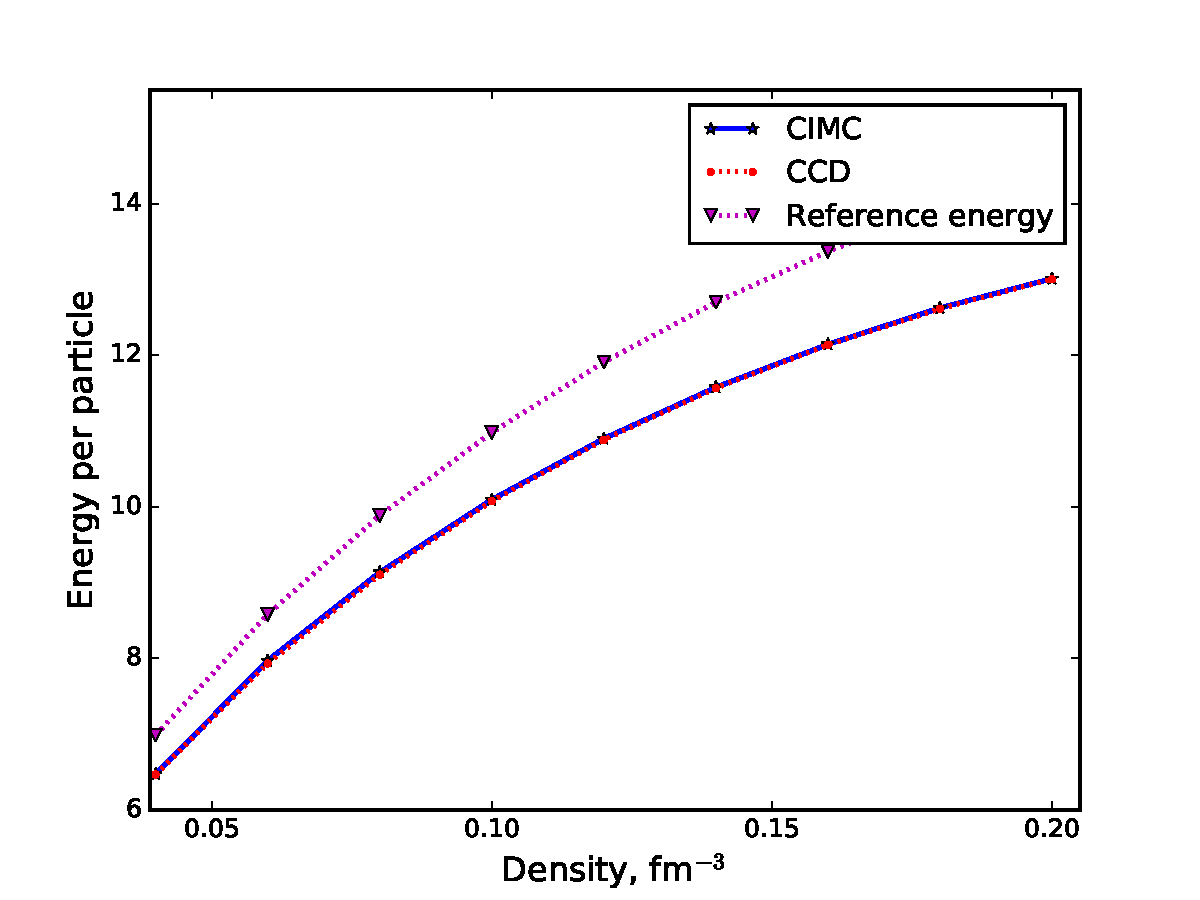
\includegraphics[scale=0.5]{Chapter9-figures/cimcccd.pdf}
	\end{center}
	\caption{Equation of state of neutron matter modeled as a periodic cell containing A=66 neutrons using the CIMC method and coupled cluster theory with doubes correlations. Single-particle states up to $N_{\mathrm{max}}=36$ have been included.}
	\label{fig.cimc_eos}
\end{figure}

In Fig. \ref{fig.cimc_eos} the energy computed by CIMC shown for the same neutron matter model as a function of the density (the so called "Equation of State" of neutron matter) is compared with the coupled theory results with doubles (CCD) only discussed in the previous chapter. 
In this calculation single-particle states up to $N_{\mathrm{max}}=36$ have been used. The CIMCC and CCD results are converged to the fifth digit as function of 
$N_{\mathrm{max}}$. The agreement between the two methods is at the level of the third digit after the decimal point for neutron matter with the 
Minnesota interaction. This is a striking agreement between such different many-body methods, in particular for larger densities where correlations and contributions from states above and below the Fermi level play a larger role, as seen from the difference between the reference energy and the CIMC and CCD energies.
Most likely, there will be larger differences between different many-body methods when proton correlations are brought in, as well as when more realistic interaction models will be used. Such results will be presented elsewhere. In the next two chapters we will add results using two  additional many-body methods, the in-medium SRG approach described in chapter 10 and the Green's function approach of chapter 11.  

\section{Conclusions and perspectives}

Quantum Monte Carlo methods are still one of the most powerful tools to attack general many body problems, and in particular the many-nucleon problem. Despite the fact that the Fermion sign problem prevents us so far from having strictly exact results for the solution of the Schr\"odinger equation, the accuracy that can be reached is very high, and in any cases it constitutes the current benchmark.

Another important general feature of QMC calculations is that they provide a very flexible framework in which it is possible to explore from low temperature condensed helium, to trapped fermions, from atoms and molecules ad solid state devices to nuclei and eventually lattice QCD. It is not rare that technical improvements spread across different disciplines, and the development of te method itself is a common ground that is often the subject of interdisciplinary workshops and conferences.  

In the field of nuclear physics it is possible that Fock-space based methods will eventually become the standard. Their main feature is the possibility of dealing with non-local interactions, which makes it possible to extend the use of QMC to the original formulations of $\xi$-EFT potentials, and a whole class of soft-core interactions that so far have never been used in this context. On the other hand, the availability of more and more accurate versions of the AFDMC codes will open the access of accurate studies of the equation of state f neutron and nuclear matter, and of general baryonic matter of extreme importance for astrophysical applications, concerning in particular the physics of neutron stars. The possibility of extending accurate calculations to large $A$ systems is also crucial for understanding the phenomenology of exotic beams.

In this chapter we did not deal with the problem of evaluating excited states and dynamical quantities within a QMC framework. Several methods are nowadays available, mostly based on the evaluation of the Laplace transform of a given response function by means of the calculation of imaginary time correlation functions. Many technical advances have been recently made in this field (see e.g. Refs. \cite{Galli, RoggeroHe, Lovato1,Lovato2}), and the subject is still under very active investigation. 

Finally, the hardest wall to climb remains the solution of the Fermion sign problem. Although there are claims that the problem is NP complete (which is true in general), thereby preventing any solution within standard classical computation, there are hints that many Hamiltonians of interest might admit a viable solution with polynomial scaling in $A$. This problem would definitely deserve more efforts than those that are presently devoted to its solution.  
\section{Problems}
 \begin{prob}
  Evaluate the following integral by means of the Metropolis algorithm
  \[
  I=\int_0^1 e^{x}-1\, dx
  \]
  sampling points from
  \begin{enumerate}
  	\item P(x) = 1 for $x\in[0,1]$
  	\item P(x) = x for $x\in[0,1]$
  \end{enumerate}
  \begin{itemize}
  	\item
  Compare the average and the statistical error for the cases 1) and 2). Which is the best estimate?
  \item
  Try to figure out a way to sample a probability density proportional to $x^n$, and reevaluate the integral
  $I$. How is the convergence and the statistical error behaving by increasing $n$? Try to give an explanation of the result.  
  \end{itemize}
  \end{prob}
  \begin{prob}
  Try to sketch the general proof that for a generic integral $I$ defined as in problem 9.1 the best statistical error is obtained when sampling from a probability density proportional to F(x).
  \end{prob}
  \begin{prob}
  Consider the one-dimensional Hamiltonian:
  \[
  \hat{H}=\frac{1}{2}\frac{d^2}{dx^2}+\frac{1}{2}x^2
  \]
  and consider the parametrized family of trial solutions $\psi(x,\alpha,\beta)=e^{-\alpha^2 x^2}-\beta$. Compute by means of the  Metropolis algorithm the energy and the standard deviation of the energy as a function of $\alpha$ keeping $\beta=0.01$. Is the minimum found at the same value than for $\beta =0$? Why?
  \end{prob}
  \begin{prob}
  	Prove that the propagator defined in the integrand of Eq.(\ref{free_propagator}) is the Green's function of the differential equation (\ref{diffusion_eq}).
  \end{prob}
  \begin{prob}
  \label{prob:egamma}
	Show that the given two fixed-phase energies $E_{a}$ and $E_{b}$ obtained using the hamiltonians $\mathcal{H}_{\gamma}$ defined in Eq.~(\eqref{mh1}) and Eq.~(\eqref{mh2}) 
	with $\gamma=a$ and $\gamma=b$ ($a,b\geq 0$) the linear extrapolation to $\gamma=-1$ (remember that $\mathcal{H}_{-1}=H$) is still an upper bound. 
	(Hint: show that $E_\gamma$ is a convex function of the parameter $\gamma$).
  \end{prob}
  \begin{prob}
  \label{prob:heatbath}
        Implement the function $HeatBath[P,\mathbf{n}]$ that appears in the algorithm EXP\_Move() in Sec.~\ref{sec:expprop}.
  \end{prob}
\begin{prob}
In the case of nuclear Hamiltonians spin is not a conserved quantity. Referring to the calculation of the local energy in Sec. 9.6.4, how would you modify the subroutine EL\_calc2 to take into account the non-conservation of spin?
\end{prob}
  

\section*{Appendix}
\addcontentsline{toc}{section}{Appendix}
In this appendix we give the proof of the upper--bound property for the auxiliary hamiltonians $\mathcal{H}_{\gamma}$, defined in Sec.~\ref{subsect:CCDMC-IS}, for
the general complex--hermitian case (see \cite{TenHaaf95} for the original proof in the real symmetric case).
We will concentrate in the simpler case $\gamma=0$ in equations \eqref{mh1} and \eqref{mh2}, extension to the generic $\gamma \geq 0$ is then straightforward. In what follows
 we will use the shorthand $\mathcal{H}_{\gamma=0} \equiv \widetilde{H}$. Let $\Psi(\mathbf{n})$ be any arbitrary wave function, our goal is to show that 
\begin{equation}
\Re [\langle \Psi \lvert \widetilde{H}\rvert\Psi \rangle]\geq\Re\left[ \langle \Psi |H|\Psi \rangle\right]\;. 
\end{equation}

Let us proceed by considering the following difference:
\begin{equation}
\begin{split}
 \Re [\langle \Psi& \lvert \widetilde{H}\rvert\Psi \rangle] -\Re\left[ \langle \Psi |H|\Psi \rangle\right]=  \sum_{\mathbf{m}\mathbf{n}} \Re \left[\Psi^*(\mathbf{m}) (\widetilde{H}_{\mathbf{m}\mathbf{n}}-H_{\mathbf{m}\mathbf{n}})\Psi(\mathbf{n})\right]\\ 
&= \sum_{\mathbf{m}\mathbf{n}} h_{\mathbf{m}\mathbf{n}}  \lvert\Psi(\mathbf{n})\rvert^2 +\sum_{\mathbf{m}\neq \mathbf{n}}  \Re \left[\Psi^*(\mathbf{m}) (\widetilde{H}_{\mathbf{m}\mathbf{n}}-H_{\mathbf{m}\mathbf{n}})\Psi(\mathbf{n})\right]\\
&= \sum_{\mathbf{n}} \sum_{\mathfrak{s}_{\mathbf{m}\mathbf{n}} \neq -} \lvert\Psi(\mathbf{n})\rvert^2  \frac{\Re \left [ \Phi_T^*(\mathbf{m}) H_{\mathbf{m}\mathbf{n}} \Phi_T(\mathbf{n})\right ]}{ \lvert \Phi_T (\mathbf{n}) \rvert ^2} - \Re \left [ \Psi^*(\mathbf{m}) H_{\mathbf{m}\mathbf{n}} \Psi(\mathbf{n})\right ]\\ 
%&= \sum_n \sum_{s_{mn} \neq -} \lvert\Psi(n)\rvert^2  (-p_{mn}) - \Re \left [ \Psi^*(m) \Phi(m) \Phi(m)^{-1} H_{mn} \Phi^*(n)^{-1}\Phi^*(n)\Psi(n)\right ]
\end{split}
\end{equation}
where the second sum is over all ${\mathbf{m}\mathbf{n}}$ pairs such that $\mathfrak{s}_{\mathbf{m}\mathbf{n}}$ of \eqref{CCDMC:ham_sign} is positive--definite. The last term
 can now be rewritten as:
\begin{equation}
\begin{split}
\Re \left [ \Psi^*(\mathbf{m}) H_{\mathbf{m}\mathbf{\mathbf{n}}} \Psi(\mathbf{\mathbf{n}})\right ] &= \Re \left [ \Psi^*(\mathbf{m}) \Phi_T(\mathbf{m}) \Phi_T(\mathbf{m})^{-1} H_{\mathbf{m}\mathbf{n}} \Phi_T^*(\mathbf{n})^{-1}\Phi_T^*(\mathbf{n})\Psi(\mathbf{n})\right ]\\
&= (\Psi^*(\mathbf{m}) \Phi(\mathbf{m}))\Re \left [\Phi_T(\mathbf{m})^{-1} H_{\mathbf{m}\mathbf{n}} \Phi_T^*(\mathbf{n})^{-1}\right ] (\Phi_T^*(\mathbf{n})\Psi(\mathbf{n}))\\
&= (\Psi^*(\mathbf{m}) \Phi(\mathbf{m}))\Re \left [\frac{\Phi_T^*(\mathbf{m})}{\lvert\Phi_T(\mathbf{m})\rvert^2} H_{\mathbf{m}\mathbf{n}} \frac{\Phi_T(\mathbf{n})}{\lvert\Phi_T(\mathbf{n})\rvert^2}\right ] (\Phi_T^*(\mathbf{n})\Psi(\mathbf{n}))\\
\end{split}
\end{equation}
where in the second step we used the fact that by employing a real propagator we are imposing a fixed--phase constraint,  ie $\Im (\Phi_T^*(\mathbf{n})\Psi(\mathbf{n})) = 0$ for every $\mathbf{n}$ explored in the random walk. The equation for the difference becomes:
\begin{equation}
\begin{split}
 \Re [\langle \Psi& \lvert \widetilde{H}\rvert\Psi \rangle] -\Re\left[ \langle \Psi |H|\Psi \rangle\right]=  \sum_{\mathbf{m}\mathbf{n}} \Re \left[\Psi^*(\mathbf{m}) (\widetilde{H}_{\mathbf{m}\mathbf{n}}-H_{\mathbf{m}\mathbf{n}})\Psi(\mathbf{n})\right]\\ 
&= \sum_{\mathbf{n}} \sum_{\mathfrak{s}_{\mathbf{m}\mathbf{n}} \neq -} \frac{\Re \left [ \Phi_T^*(\mathbf{m}) H_{\mathbf{m}\mathbf{n}} \Phi_T(\mathbf{n})\right ]}{ \lvert \Phi_T (\mathbf{n}) \rvert ^2}\left( \lvert\Psi(\mathbf{n})\rvert^2  - \frac{(\Psi^*(\mathbf{m}) \Phi_T(\mathbf{m}))  (\Phi_T^*(\mathbf{n})\Psi(\mathbf{n}))}{\lvert\Phi(\mathbf{m})\rvert^2 }\right) \;.\\
\end{split}
\end{equation}

Using again the fixed--phase constraint (ie. $(\Phi_T^*(\mathbf{n})\Psi(\mathbf{n})) \equiv (\Phi_T(\mathbf{n})\Psi^*(\mathbf{n}))$) we can rewrite the numerator of the second term as:
\begin{equation}
\begin{split}
(\Psi^*(\mathbf{m}) \Phi_T(\mathbf{m}))  (\Phi_T^*(\mathbf{n})\Psi(\mathbf{n})) &= -\frac{1}{2} \big( \lvert \Psi^*(\mathbf{m}) \Phi_T(\mathbf{n}) - \Phi_T^*(\mathbf{m})\Psi(\mathbf{n})\rvert^2 \\
&\quad- \lvert \Phi_T(\mathbf{n})\rvert^2\lvert \Psi(\mathbf{m})\rvert^2 -\lvert \Phi_T(\mathbf{m})\rvert^2\lvert \Psi(\mathbf{n})\rvert^2 \big)\\
\end{split}
\end{equation}
and then we have:
\begin{equation}
\begin{split}
 \Re \left[\langle \Psi \lvert \widetilde{H}\rvert\Psi \rangle\right] & -\Re\left[ \langle \Psi |H|\Psi \rangle\right]=  \sum_{\mathbf{m}\mathbf{n}} \Re \left[\Psi^*(\mathbf{m}) (\widetilde{H}_{\mathbf{m}\mathbf{n}}-H_{\mathbf{m}\mathbf{n}})\Psi(\mathbf{n})\right]\\ 
&= \sum_{\mathbf{n}} \sum_{\mathfrak{s}_{\mathbf{m}\mathbf{n}} \neq -} \frac{\Re \left [ \Phi_T^*(\mathbf{m}) H_{\mathbf{m}\mathbf{n}} \Phi_T(\mathbf{n})\right ]}{ \lvert \Phi_T(\mathbf{n}) \rvert ^2}\bigg( \lvert\Psi(\mathbf{n})\rvert^2  + \frac{ \lvert \Psi^*(\mathbf{m}) \Phi_T(\mathbf{n}) - \Phi_T^*(\mathbf{m})\Psi(\mathbf{n})\rvert^2}{2 \lvert\Phi_T(\mathbf{m})\rvert^2} \\  
&- \frac{ \lvert \Phi_T(\mathbf{n})\rvert^2\lvert \Psi(\mathbf{m})\rvert^2}{2\lvert\Phi_T(\mathbf{m})\rvert^2}- \frac{ \lvert \Psi(\mathbf{n})\rvert^2}{2}\bigg)\\
&= (\mbox{positive terms}) + \sum_{\mathbf{n}} \sum_{\mathfrak{s}_{\mathbf{m}\mathbf{n}} \neq -} \frac{\Re \left [ \Phi_T^*(\mathbf{m}) H_{\mathbf{m}\mathbf{n}} \Phi_T(\mathbf{n})\right ]}{ 2\lvert \Phi_T(\mathbf{n}) \rvert ^2}\left( \lvert\Psi(\mathbf{n})\rvert^2  - \frac{ \lvert \Phi_T(\mathbf{n})\rvert^2\lvert \Psi(\mathbf{m})\rvert^2}{\lvert\Phi_T(\mathbf{m})\rvert^2} \right) \\  
\end{split}
\end{equation}
Now we note that 
\begin{equation*}
\Re \left [ \Phi_T^*(\mathbf{m}) H_{\mathbf{m}\mathbf{n}} \Phi_T(\mathbf{n})\right ] = \Re \left [ \Phi_T^*(\mathbf{n}) H_{\mathbf{n}\mathbf{m}} \Phi_T(\mathbf{m})\right ]
\end{equation*}
for a complex--hermitian hamiltonian, we can then express the sums by allowing only unique $\mathbf{m}\mathbf{n}$ combinations:
\begin{equation}
\begin{split}
 \Re \left[\langle \Psi \lvert \widetilde{H}\rvert\Psi \rangle\right] & -\Re\left[ \langle \Psi |H|\Psi \rangle\right]=  \sum_{\mathbf{m}\mathbf{n}} \Re \left[\Psi^*(\mathbf{m}) (\widetilde{H}_{\mathbf{m}\mathbf{n}}-H_{\mathbf{m}\mathbf{n}})\Psi(\mathbf{n})\right]\\ 
&= (\mbox{positive terms}) + \\
&\sum_{\mathbf{n}} \sum'_{\mathfrak{s}_{\mathbf{m}\mathbf{n}} \neq -} \Re \left [ \Phi_T^*(\mathbf{m}) H_{\mathbf{m}\mathbf{n}} \Phi_T(\mathbf{n})\right ] \bigg( \frac{\lvert\Psi(\mathbf{n})\rvert^2}{2\lvert\Phi_T(\mathbf{n})\rvert^2} + \frac{\lvert\Psi(\mathbf{m})\rvert^2}{2\lvert\Phi_T(\mathbf{m})\rvert^2}-\\
& \frac{ \lvert \Phi_T(\mathbf{n})\rvert^2\lvert \Psi(\mathbf{m})\rvert^2}{2\lvert\Phi_T(\mathbf{m})\rvert^2 \lvert \Phi_T(\mathbf{n})\rvert^2} - \frac{ \lvert \Phi_T(\mathbf{m})\rvert^2\lvert \Psi(\mathbf{n})\rvert^2}{2 \lvert \Phi_T(\mathbf{n})\rvert^2\lvert\Phi_T(\mathbf{m})\rvert^2} \bigg)\\
&=  (\mbox{positive terms})
\end{split}
\end{equation}
which by definition is positive. The extension to the case with $\gamma>0$ is straightforward since we are basically adding a positive constant to the difference.

\begin{thebibliography}{99.}%
\bibitem{Kalos08}
M.H. Kalos and P.A Whitlock, {\em Monte Carlo Methods} (Wiley-VCH, 2008)
\bibitem{Metropolis53}
N. Metropolis, A. W. Rosenbluth, M. N. Rosenbluth, A. H. Teller and E. Teller,  J. Chem. Phys. {\bf 21}, 1087 (1953)
\bibitem{Hastings70}
W. K. Hastings,  Biometrika {\bf 57}, 97 (1970)
\bibitem{Cep77}
D. Ceperley, G. V. Chester, and M. H. Kalos, Phys. Rev. B {\bf 16}, 3081 (1977)
\bibitem{Cyrus96}
M.P. Nightingale and C.J. Umrigar, in \emph{"Recent Advances in Quantum Monte Carlo Methods"}, edited by W.A. Lester, Jr., (World Scientific, 1996)
\bibitem{Toulouse07}
J. Toulouse and C. J. Umrigar,  J. Chem. Phys. {\bf 126}, 084102 (2007)
\bibitem{Sorella01}
S. Sorella,  Phys. Rev. B {\bf 64}, 024512 (2001)
\bibitem{Sarsa00}
A. Sarsa, K. E. Schmidt and W. R. Magro, J. Chem. Phys. {\bf 113}, 1366 (2000)
\bibitem{Anderson76}
J. B. Anderson,  J. Chem. Phys. {\bf 65}, 4121 (1976)
\bibitem{Troyer05}
M. Troyer and U.-J. Wiese,  Phys. Rev. Lett. {\bf 94}, 170201 (2005)
\bibitem{Kalos00}
M. H. Kalos and F. Pederiva, Phys. Rev. Lett. {\bf 85}, 3547 (2000)
\bibitem{Assaraf07}
R. Assaraf, M. Caffarel and A. Khelif,  J. Phys. A Math. Theor. {\bf 40}, 1181 (2007)
\bibitem{Ceperley80}
D. M. Ceperley and B. J. Alder, Phys. Rev. Lett. {\bf 45}, 566 (1980)
\bibitem{Foulkes01}
W. M. C. Foulkes, L. Mitas, R. J. Needs, and G. Rajagopal, Rev. Mod. Phys. 73, 33 (2001)
\bibitem{Ortiz93}
G. Ortiz, D. M. Ceperley, and R. M. Martin, Phys. Rev. Lett. {\bf 71}, 2777 (1993)
\bibitem{carlson1993}
J. Carlson, V. R. Pandharipande, and R. Schiavilla,
Phys. Rev. C {\bf 47}, 484 (1993) 
\bibitem{Zhang2003}
S. Zhang and H. Krakauer,  Phys. Rev. Lett. {\bf 90}, 136401 (2003)
\bibitem{Booth09}
G. H. Booth, A. J. W. Thom, and A. Alavi,  J. Chem. Phys. {\bf 131}, 054106 (2009)
\bibitem{Cleland10}
D. Cleland, G. H. Booth, and A. Alavi, J. Chem. Phys. {\bf 132}, 041103 (2010)
\bibitem{Petruzielo12} F. R. Petruzielo, A. A. Holmes, H. J. Changlani, M. P.
Nightingale, and C. J. Umrigar, Phys. Rev. Lett. {\bf 109}, 230201 (2012)
\bibitem{Booth13}
G. H. Booth, A. Gr\"uneis, G. Kresse, and A. Alavi, Nature
{\bf 493}, 365 (2013)
\bibitem{Mukherjee13}
A. Mukherjee and Y. Alhassid,  Phys. Rev. A {\bf 88}, 053622 (2013)
\bibitem{Roggero13}
A. Roggero, A. Mukherjee, and F. Pederiva, Phys. Rev. B {\bf 88}, 115138 (2013)
\bibitem{Roggero14}
A. Roggero, A. Mukherjee, and F. Pederiva, Phys. Rev. Lett. {\bf 112}, 221103 (2014)
\bibitem{Trivedi90}
N. Trivedi and D. M. Ceperley, Phys. Rev. B {\bf 41}, 4552 (1990)
\bibitem{Sorella00}
S. Sorella and L. Capriotti,  Phys. Rev. B {\bf 61}, 2599 (2000)
\bibitem{TenHaaf95}
D. F. B. ten Haaf, H. J. M. van Bemmel, J. M. J. van Leeuwen, W. van Saarloos and D. M. Ceperley,  Phys. Rev. B {\bf 51}, 13039 (1995)
\bibitem{Rrapaj16}
E. Rrapaj, A. Roggero, and J. W. Holt, Phys. Rev. C {\bf 93}, 065801 (2016)
\bibitem{Kalos74}
M. H. Kalos, D. Levesque, and L. Verlet,  Phys. Rev. A {\bf 9}, 2178 (1974)
\bibitem{Holmes16}
A. Holmes, H. J. Changlani and C.J. Umrigar, J. Chem. Theory Comput. {\bf 12}, 1561 (2016)
\bibitem{Kolodrubetz12}
M. Kolodrubetz and B. K. Clark, Phys. Rev. B {\bf 86}, 075109 (2012)
\bibitem{Galli}
E. Vitali, M. Rossi, L. Reatto, and D. E. Galli,  Phys. Rev. B {\bf 82}, 174510 (2010.
\bibitem{RoggeroHe}
A. Roggero, F. Pederiva, and G. Orlandini, Phys. Rev. B {\bf 88}, 094302 (2013)
\bibitem{Lovato1}
A. Lovato, S. Gandolfi, R. Butler, J. Carlson, E. Lusk, S. C. Pieper, and R. Schiavilla,  Phys. Rev. Lett. {\bf 111}, 092501, 2013
\bibitem{Lovato2}
A. Lovato, S. Gandolfi, J. Carlson, S. C. Pieper, and R. Schiavilla, Phys. Rev. C {\bf 91},062501(R) (2015)
\end{thebibliography}
